% !TEX program = xelatex
% !BIB program = biber
% =====================================================================
% Annexes — Master en Génie Logiciel
% Projet : RohWinBghit — Plateforme de covoiturage inter-wilayas
% Université Abou Bekr Belkaïd — Tlemcen
% Année universitaire : 2025 / 2026
% Compilation : xelatex annexes_standalone.tex (deux passes)
% =====================================================================
\documentclass[12pt,a4paper,oneside]{report}

% ---------- Encodage et langues ----------
% ---------- Hyperliens ----------
\usepackage{hyperref}
\hypersetup{
  colorlinks=true,
  linkcolor=rohblue,
  citecolor=rohblue,
  urlcolor=rohblue,
  pdftitle={RohWinBghit — Annexes Master GL},
  pdfauthor={AHMED BACHA D. \& BELHORMA S.M.R.}
}

% ---------- Encodage et langues ----------
\usepackage{fontspec}
\usepackage{polyglossia}
\setmainlanguage{french}
\setotherlanguages{english}

% Bypass bidi package entirely to avoid biblatex TOC infinite loops
\TeXXeTstate=1
\newfontfamily\arabicfont[Script=Arabic,Scale=1.1,Extension=.ttf,UprightFont=Amiri-Regular,BoldFont=Amiri-Bold,ItalicFont=Amiri-Italic,BoldItalicFont=Amiri-BoldItalic]{Amiri-Regular}
\newcommand{\textarabic}[1]{{\arabicfont\beginR #1\endR}}

% ---------- Mise en page ----------
\usepackage[top=2.5cm,bottom=2.5cm,left=3cm,right=2cm]{geometry}
\setlength{\headheight}{15.21004pt}
\addtolength{\topmargin}{-3.21004pt}
\usepackage{setspace}
\onehalfspacing
\setlength{\parindent}{1.25em}
\usepackage{microtype}

% ---------- Graphisme et couleurs ----------
\usepackage{graphicx}
\graphicspath{{figures/}}
\usepackage[table]{xcolor}
\definecolor{rohblue}{RGB}{30,80,150}
\definecolor{rohlight}{RGB}{235,242,250}
\definecolor{rohaccent}{RGB}{200,60,60}

% ---------- Tableaux ----------
\usepackage{array}
\usepackage{tabularx}
\usepackage{longtable}
\usepackage{booktabs}
\usepackage{multirow}
\usepackage{colortbl}

% ---------- Listes et mise en forme ----------
\usepackage{enumitem}
\usepackage{titletoc}
\usepackage{fancyhdr}
\usepackage{float}
\usepackage{caption}
\captionsetup[figure]{labelfont={it,bf},textfont=it,labelsep=endash,font=small}
\captionsetup[table]{labelfont={it,bf},textfont=it,labelsep=endash,font=small}

% ---------- Titres de chapitres ----------
\usepackage[explicit]{titlesec}
\titleformat{\chapter}[display]
  {\normalfont\huge\bfseries\color{rohblue}}
  {\filleft\Large\scshape Annexe \thechapter}
  {0pt}
  {\vspace{0.4em}\filleft\Huge #1\vspace{-0.3em}\color{rohblue}\titlerule[1pt]}
\titlespacing*{\chapter}{0pt}{10pt}{40pt}

\titleformat{\section}
  {\color{rohblue}\Large\bfseries}{\thesection}{0.6em}{#1}
\titleformat{\subsection}
  {\color{rohblue!85}\large\bfseries}{\thesubsection}{0.6em}{#1}
\titleformat{\subsubsection}
  {\color{rohblue!70}\normalsize\bfseries}{\thesubsubsection}{0.6em}{#1}

% ---------- En-têtes / pieds de page ----------
\pagestyle{fancy}
\fancyhf{}
\fancyhead[L]{\nouppercase{\leftmark}}
\fancyhead[R]{\thepage}
\renewcommand{\headrulewidth}{0.4pt}
\fancypagestyle{plain}{\fancyhf{}\fancyfoot[C]{\thepage}\renewcommand{\headrulewidth}{0pt}}

% ---------- Code source ----------
\usepackage{listings}
\lstset{
  basicstyle=\ttfamily\small,
  keywordstyle=\color{rohblue}\bfseries,
  commentstyle=\color{gray}\itshape,
  stringstyle=\color{rohaccent},
  numbers=left, numberstyle=\tiny\color{gray},
  frame=single, rulecolor=\color{rohblue!30},
  breaklines=true, showstringspaces=false,
  tabsize=2
}

% ---------- Encadrés ----------
\usepackage{tcolorbox}
\tcbuselibrary{skins,breakable}
\newtcolorbox{highlight}[1][]{
  enhanced, breakable,
  colback=rohlight, colframe=rohblue,
  boxrule=0.5pt, arc=2pt,
  left=8pt,right=8pt,top=5pt,bottom=5pt,
  #1
}

\begin{document}

\pagenumbering{arabic}
\appendix
\chapter{Business Model Canvas}
\label{annexe:bmc}

Cette annexe présente les détails stratégiques du Business Model Canvas (BMC) de la plateforme \textit{RohWinBghit}.

\begin{itemize}
  \item \textbf{Partenaires clés :} Mapbox, Firebase, Chargily Pay, fournisseurs OTP/SMS (confirmés) ; acteurs du transport public, compagnies d'assurance, universités, incubateurs et organismes d'accompagnement à l'innovation (partenariats envisagés/potentiels).
  \item \textbf{Activités clés :} Développement logiciel et maintenance de la plateforme, vérification KYC, gestion des paiements, support utilisateur, modération, sécurité, acquisition d'utilisateurs.
  \item \textbf{Ressources clés :} Plateforme logicielle RohWinBghit, infrastructure cloud, modules d'intelligence artificielle dédiés à la vérification biométrique, données géographiques, ressources humaines, marque et propriété intellectuelle (dépôts INAPI/ONDA).
  \item \textbf{Proposition de valeur :} Plateforme de covoiturage de confiance intégrant des mécanismes avancés de vérification d'identité (KYC biométrique), paiement local, réservation sécurisée, suivi GPS, et réduction des coûts de déplacement.
  \item \textbf{Relations clients :} Confiance numérique (badge), notation mutuelle, assistance utilisateur, gestion des litiges, accompagnement KYC.
  \item \textbf{Canaux :} Application mobile (iOS/Android), site web (vitrine et console d'administration), réseaux sociaux, campus universitaires, programme d'ambassadeurs.
  \item \textbf{Segments de clientèle :} Étudiants (principal segment identifié), travailleurs actifs, conducteurs particuliers, voyageurs occasionnels.
  \item \textbf{Structure des coûts :} Infrastructure \& DevOps (VPS Cloud, base de données, GPU IA), services tiers (Mapbox, SMS OTP, Chargily Pay), ressources humaines (développement, support/modération), marketing (acquisition, parrainage).
  \item \textbf{Flux de revenus :} Commission sur les trajets, abonnement Premium conducteur, publicité ciblée, partenariats B2B.
\end{itemize}

\chapter{Diagrammes UML}
\label{annexe:uml}

\subsection*{Diagrammes de séquence secondaires}
\label{annexe:sequences_secondaires}

Cette annexe regroupe les diagrammes de séquence modélisant les interactions détaillées pour les fonctionnalités secondaires ou de support de la plateforme.

\begin{figure}[H]
\centering
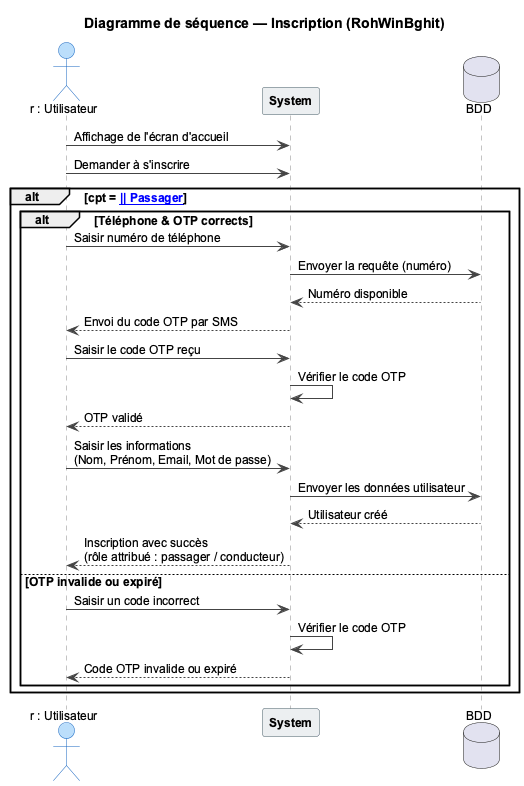
\includegraphics[width=0.85\linewidth]{fig_sequence_inscription.png}
\caption{Séquence --- Inscription d'un nouvel utilisateur}
\label{fig:seq-inscription}
\end{figure}

\begin{figure}[H]
\centering
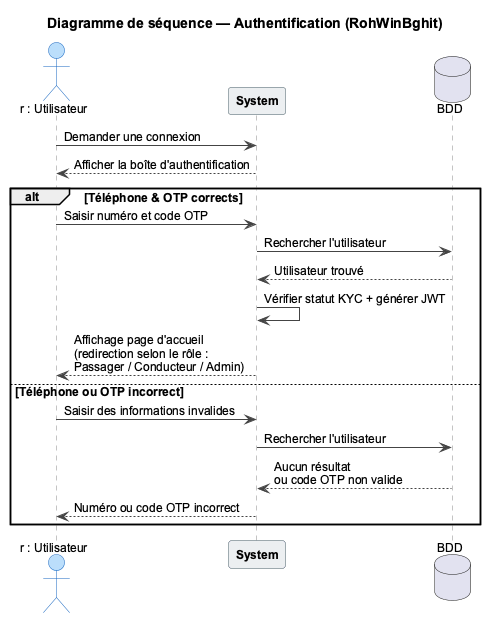
\includegraphics[width=0.95\linewidth]{fig_sequence_authentification.png}
\caption{Séquence --- Authentification et orientation par rôle}
\label{fig:seq-authentification}
\end{figure}

\begin{figure}[H]
\centering
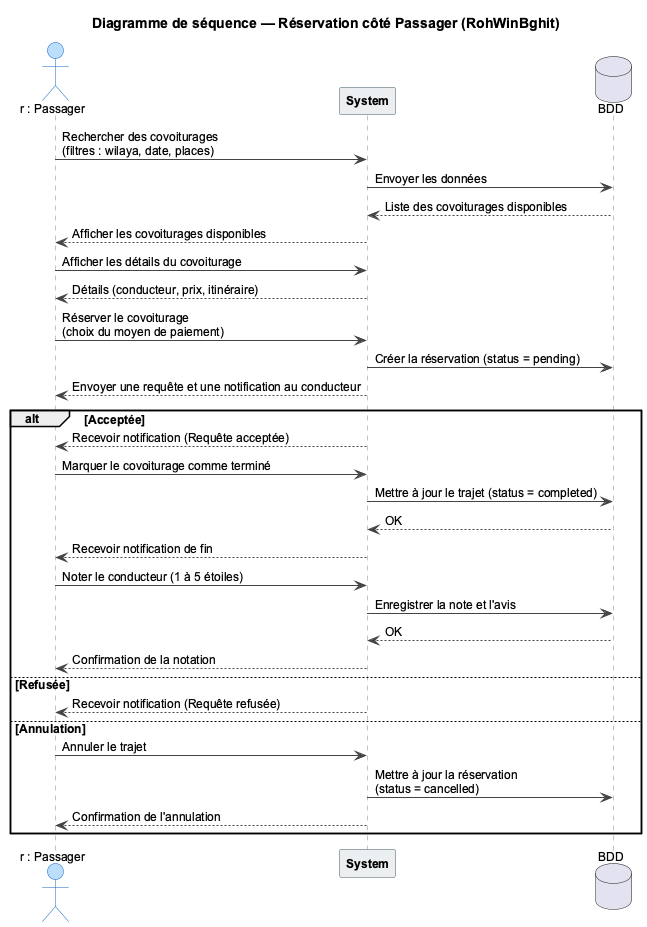
\includegraphics[width=0.95\linewidth]{fig_sequence_reservation_passager.png}
\caption{Séquence --- Réservation côté passager}
\label{fig:seq-reservation-passager}
\end{figure}

\begin{figure}[H]
\centering
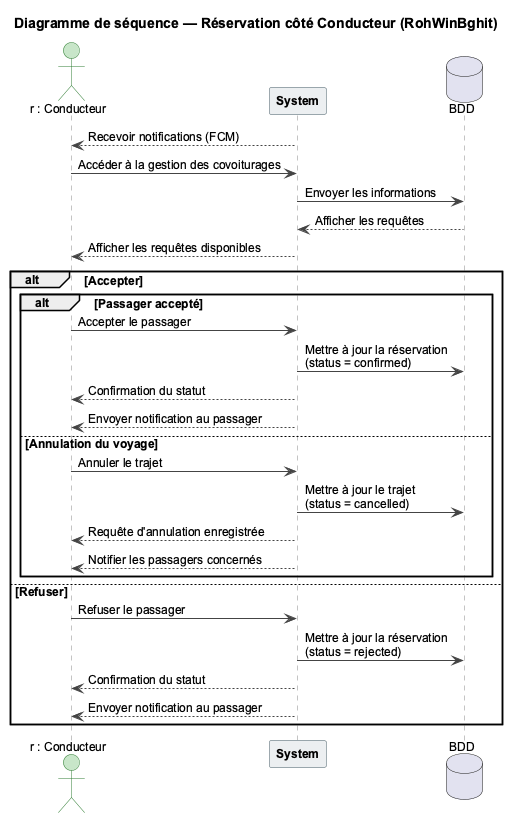
\includegraphics[width=0.95\linewidth]{fig_sequence_reservation_conducteur.png}
\caption{Séquence --- Réservation côté conducteur}
\label{fig:seq-reservation-conducteur}
\end{figure}

\begin{figure}[H]
\centering
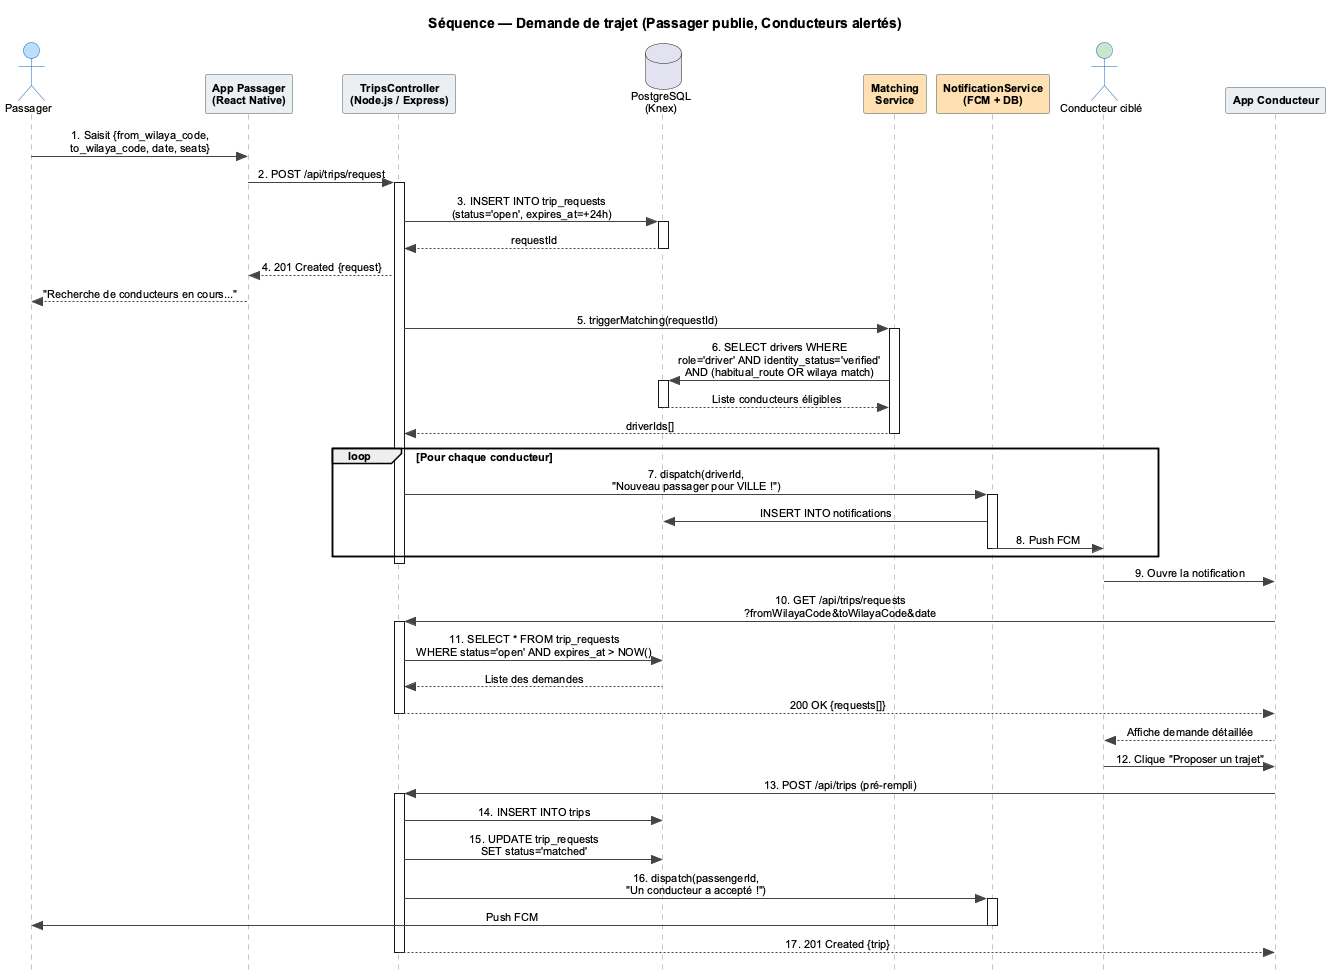
\includegraphics[width=0.95\linewidth]{fig_sequence_trip_request.png}
\caption{Séquence --- Demande de trajet (\textit{matching} passager $\to$ conducteurs)}
\label{fig:seq-trip-request}
\end{figure}




\subsection*{Diagramme d'activité global}
\label{annexe:activite_global}

Cette annexe présente le diagramme d'activité modélisant le parcours global d'un utilisateur sur la plateforme \textit{RohWinBghit}.

\begin{figure}[H]
\centering
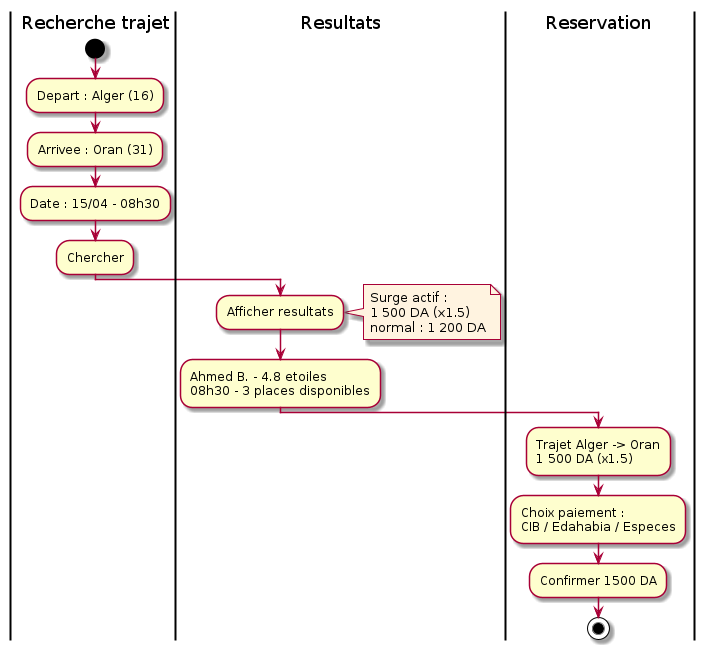
\includegraphics[width=0.85\linewidth,height=0.85\textheight,keepaspectratio]{fig_passenger_flow.png}
\caption{Diagramme d'activité --- parcours global de la plateforme}
\label{fig:activite-booking}
\end{figure}

\section*{Annexe C — Captures supplémentaires}
\addcontentsline{toc}{section}{Annexe C — Captures supplémentaires}
\label{annexe:captures}

{Catalogue complet des captures d'écran}
% captures

Ce catalogue rassemble l'intégralité des \textbf{62~écrans} de l'application mobile (31~écrans passager~+~31~écrans conducteur), ainsi que les captures du panneau d'administration.

% ----------------------------------------------------------------
\section{Parcours passager --- 31 écrans}
% ----------------------------------------------------------------

\begin{figure}[H]
\centering
\begin{minipage}{0.30\textwidth}
    \centering
    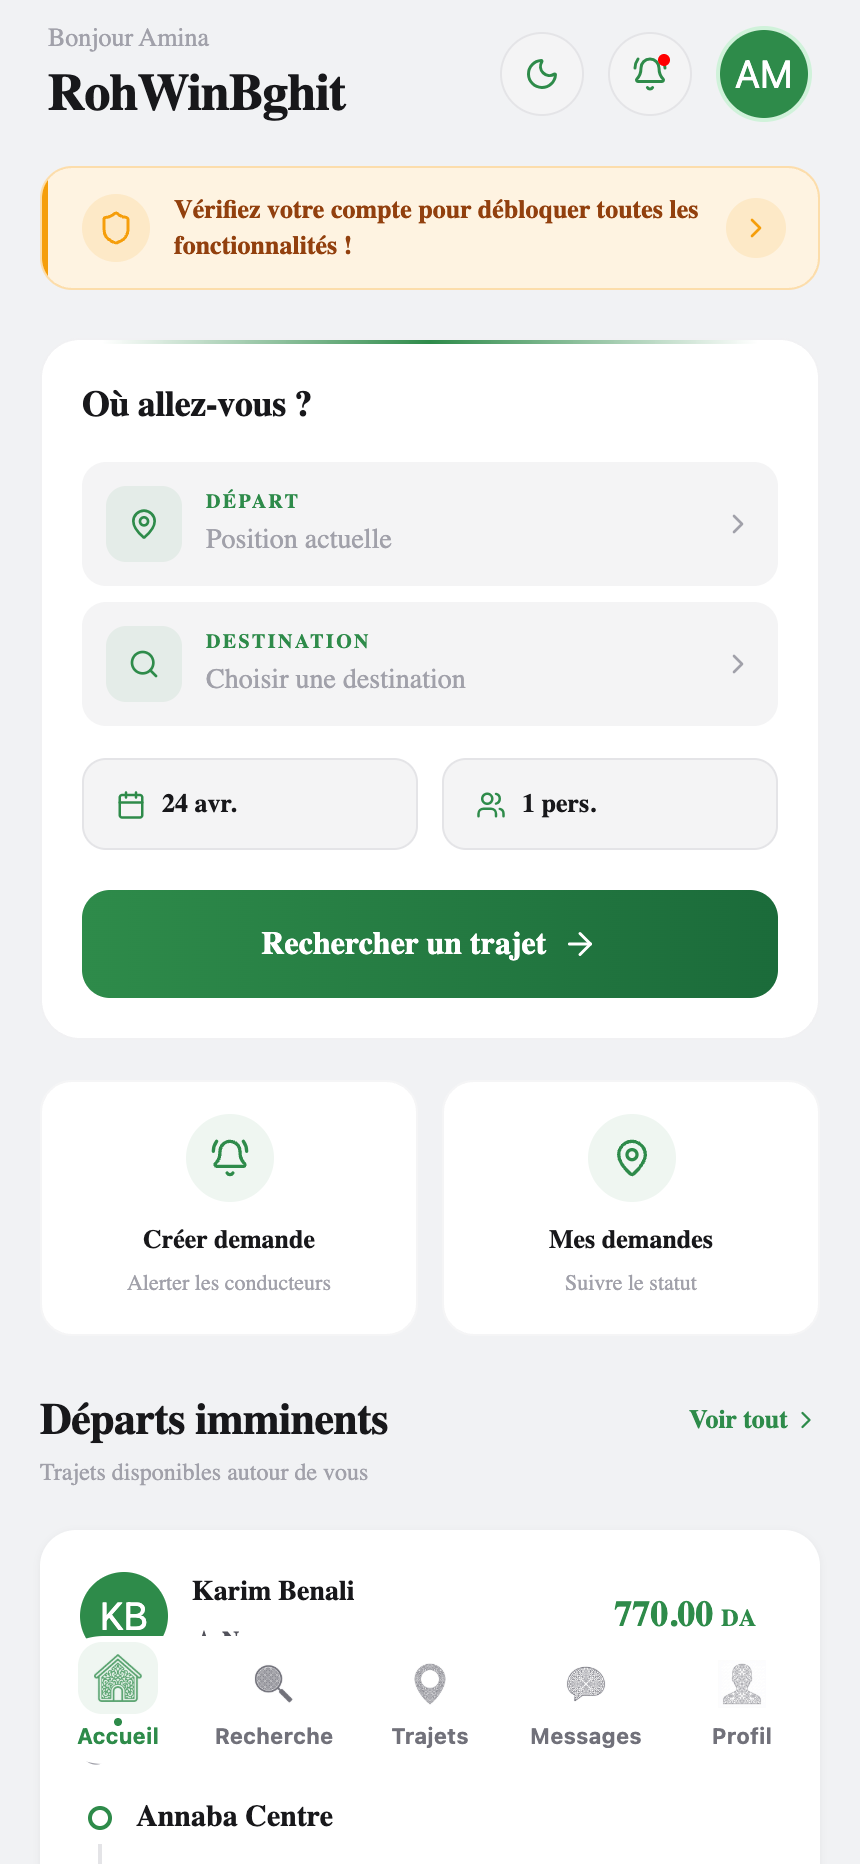
\includegraphics[width=\linewidth]{mobile-all/p_01_tab_home.png}
    {\footnotesize D.1 --- Accueil passager\par}
\end{minipage}\hfill
\begin{minipage}{0.30\textwidth}
    \centering
    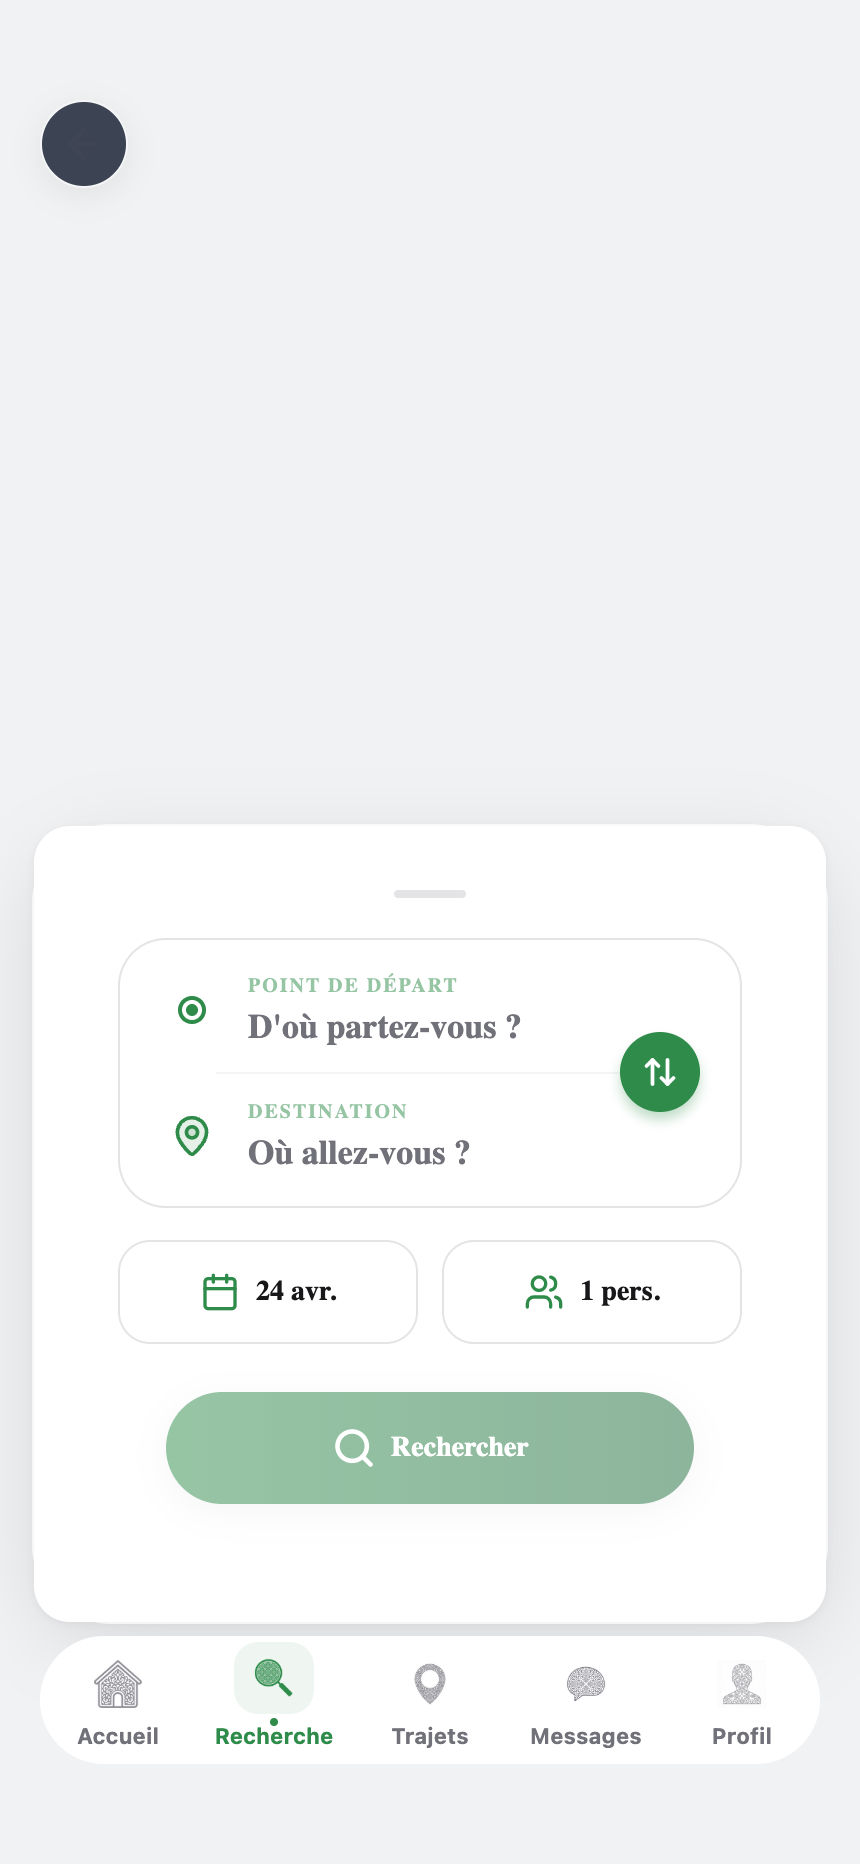
\includegraphics[width=\linewidth]{mobile-all/p_02_tab_search.png}
    {\footnotesize D.2 --- Recherche de trajet\par}
\end{minipage}\hfill
\begin{minipage}{0.30\textwidth}
    \centering
    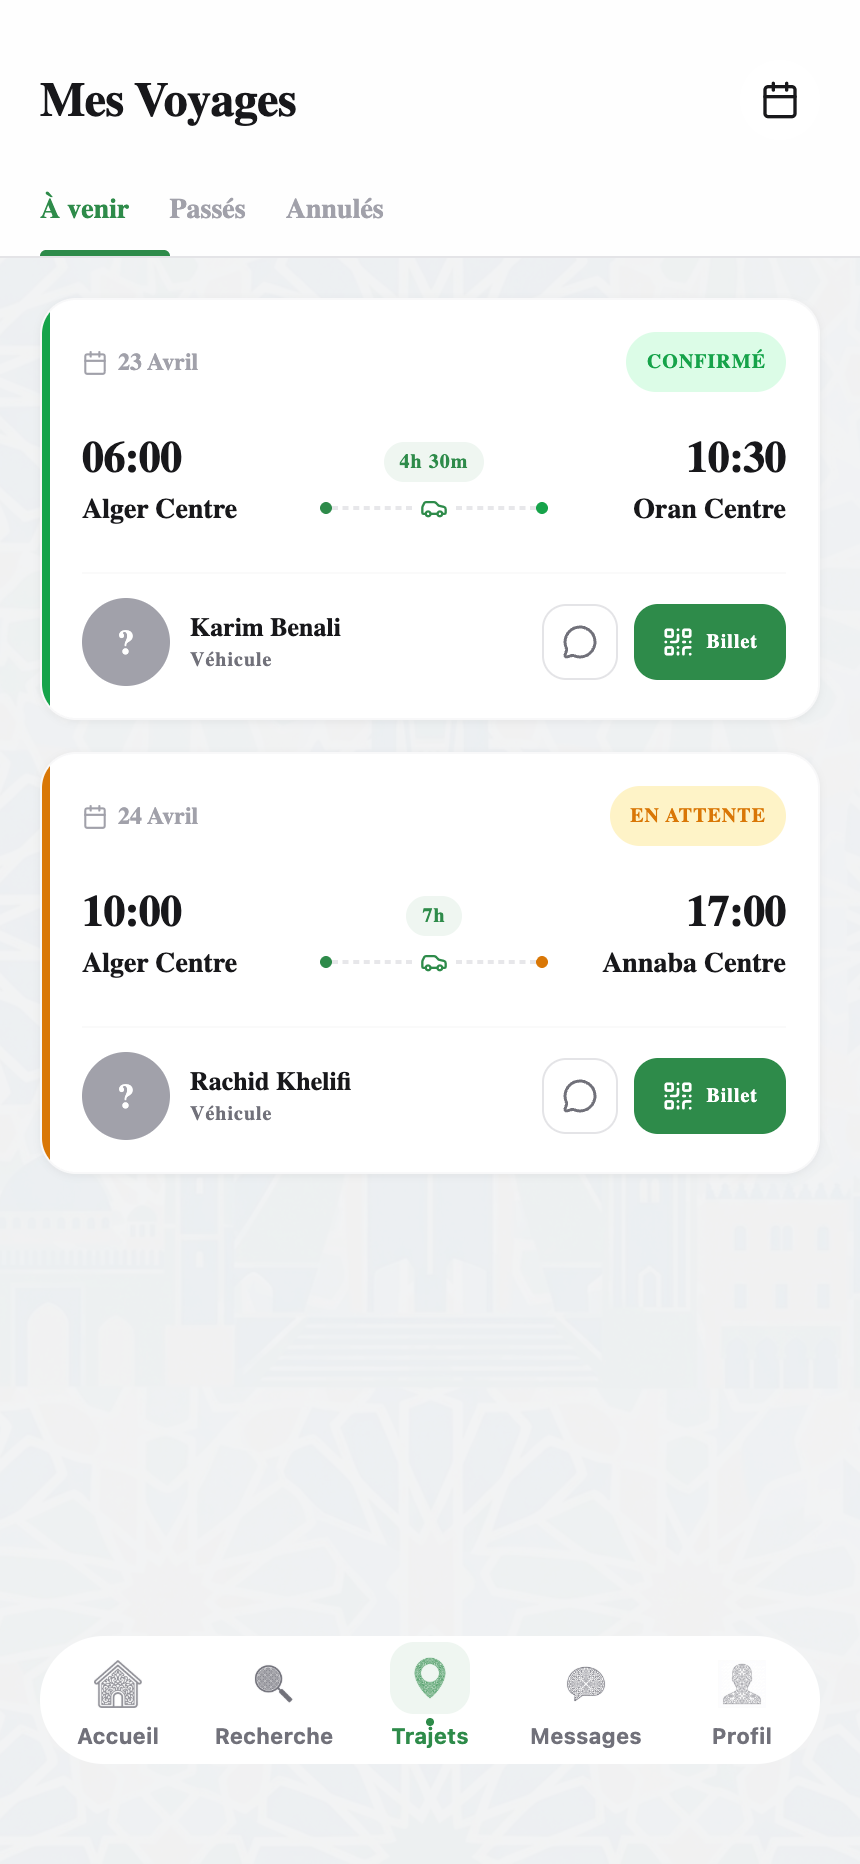
\includegraphics[width=\linewidth]{mobile-all/p_03_tab_trips.png}
    {\footnotesize D.3 --- Mes trajets\par}
\end{minipage}
\end{figure}

\begin{figure}[H]
\centering
\begin{minipage}{0.30\textwidth}
    \centering
    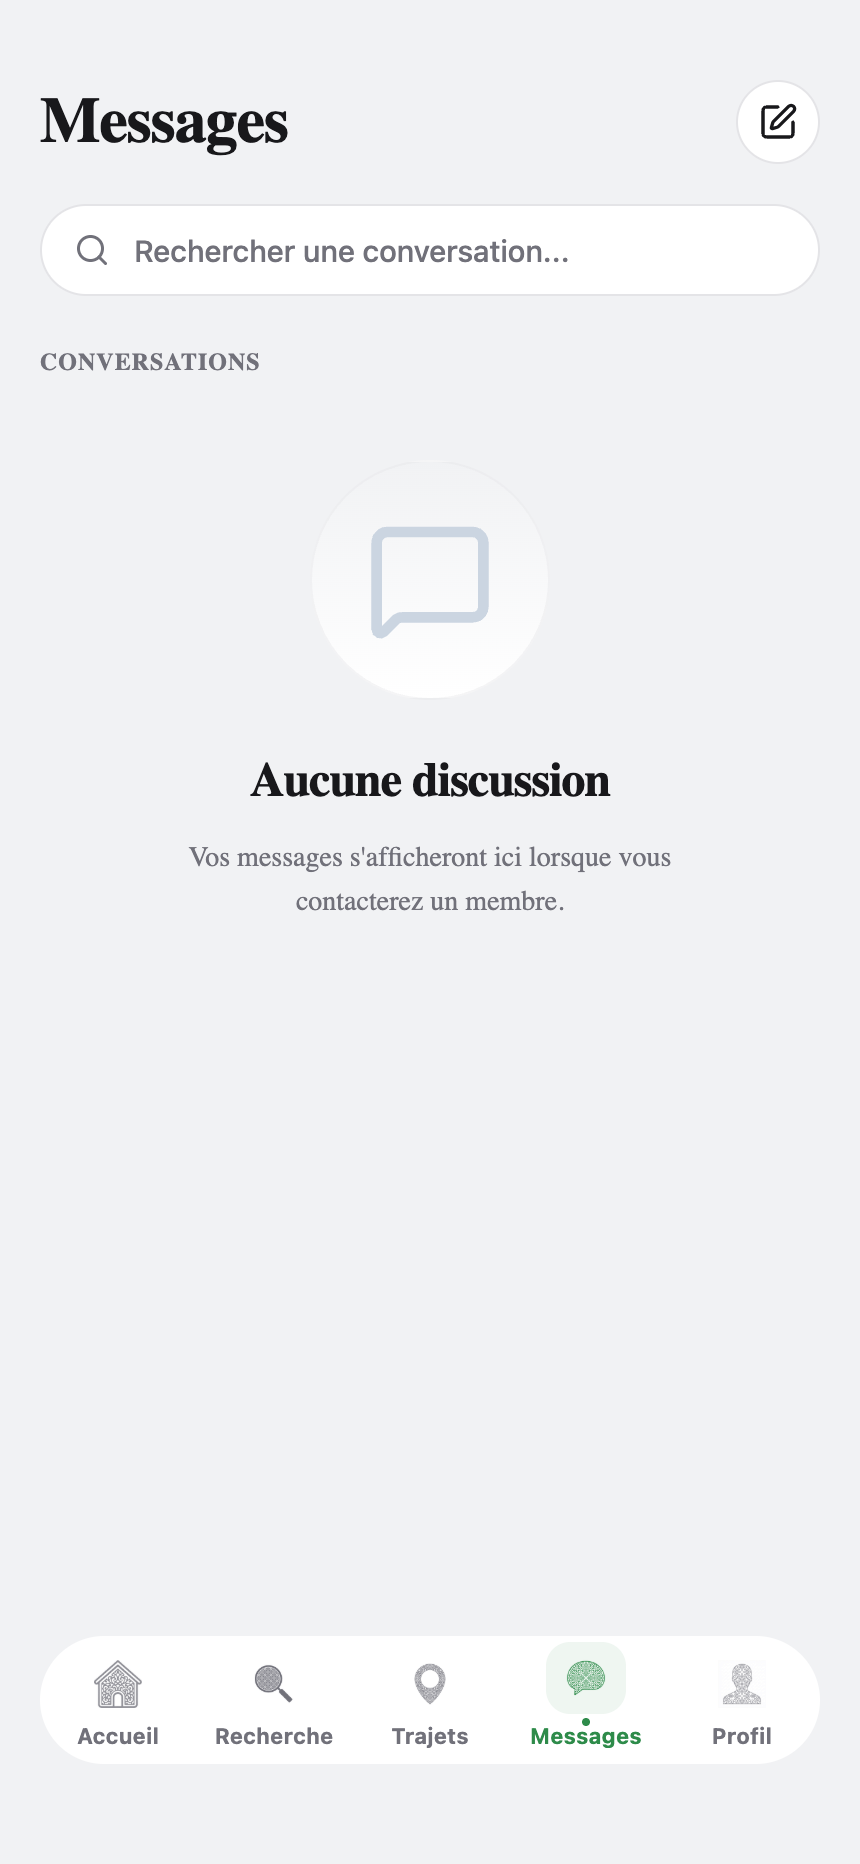
\includegraphics[width=\linewidth]{mobile-all/p_04_tab_messages.png}
    {\footnotesize D.4 --- Messagerie\par}
\end{minipage}\hfill
\begin{minipage}{0.30\textwidth}
    \centering
    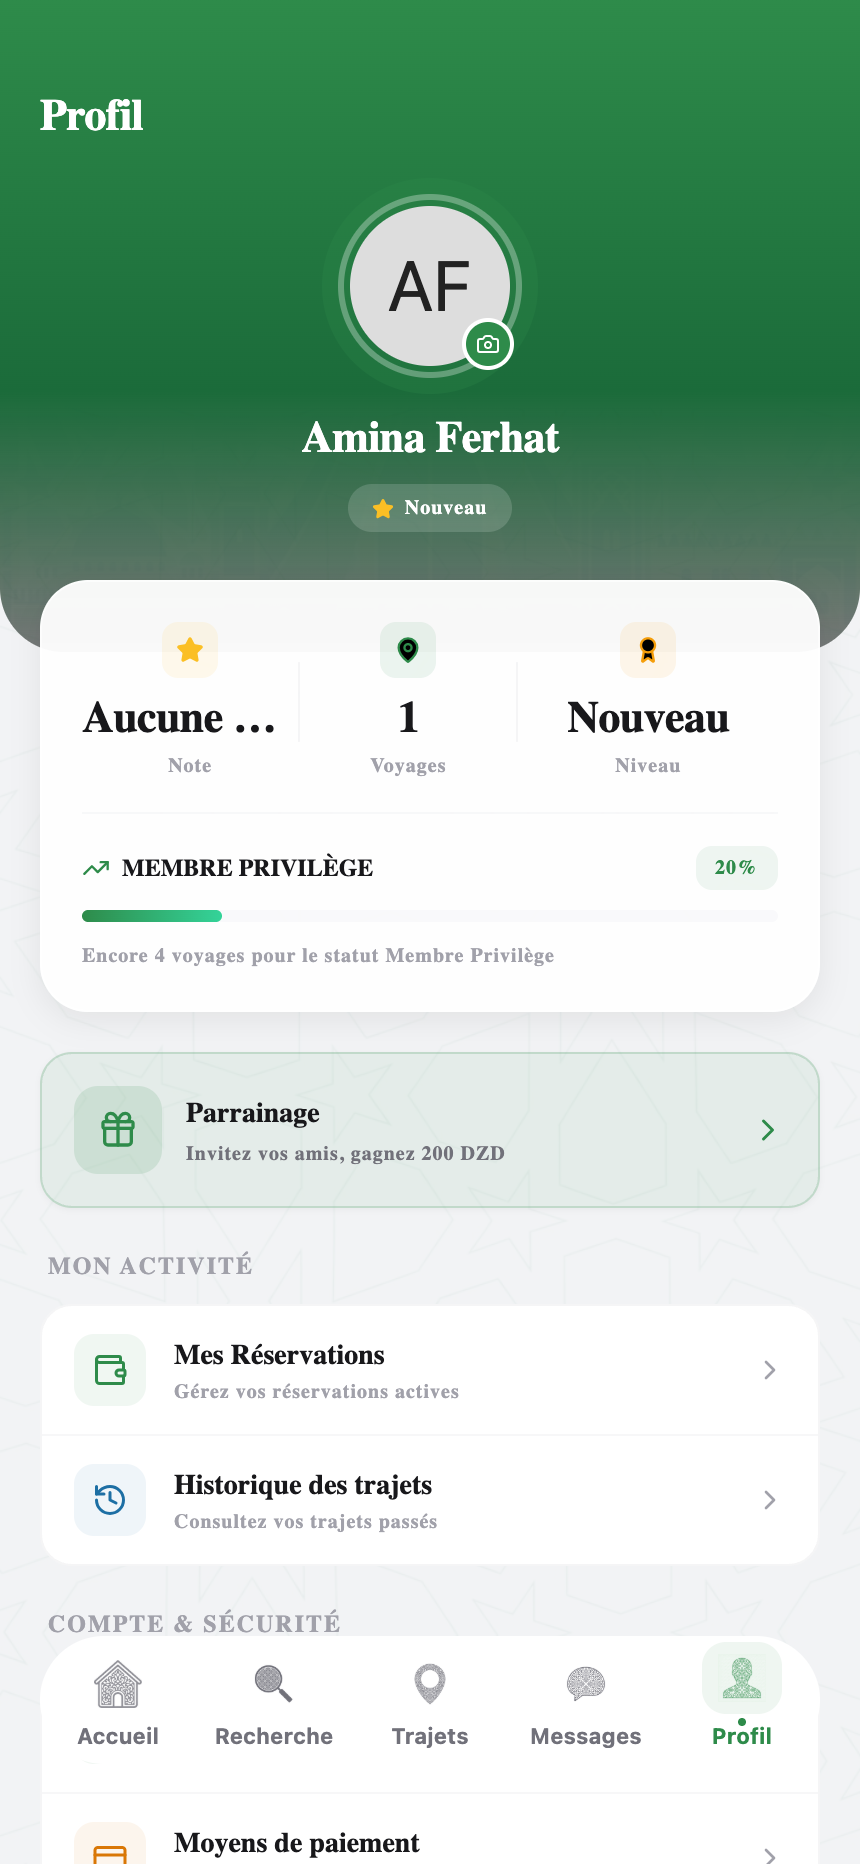
\includegraphics[width=\linewidth]{mobile-all/p_05_tab_profile.png}
    {\footnotesize D.5 --- Profil\par}
\end{minipage}\hfill
\begin{minipage}{0.30\textwidth}
    \centering
    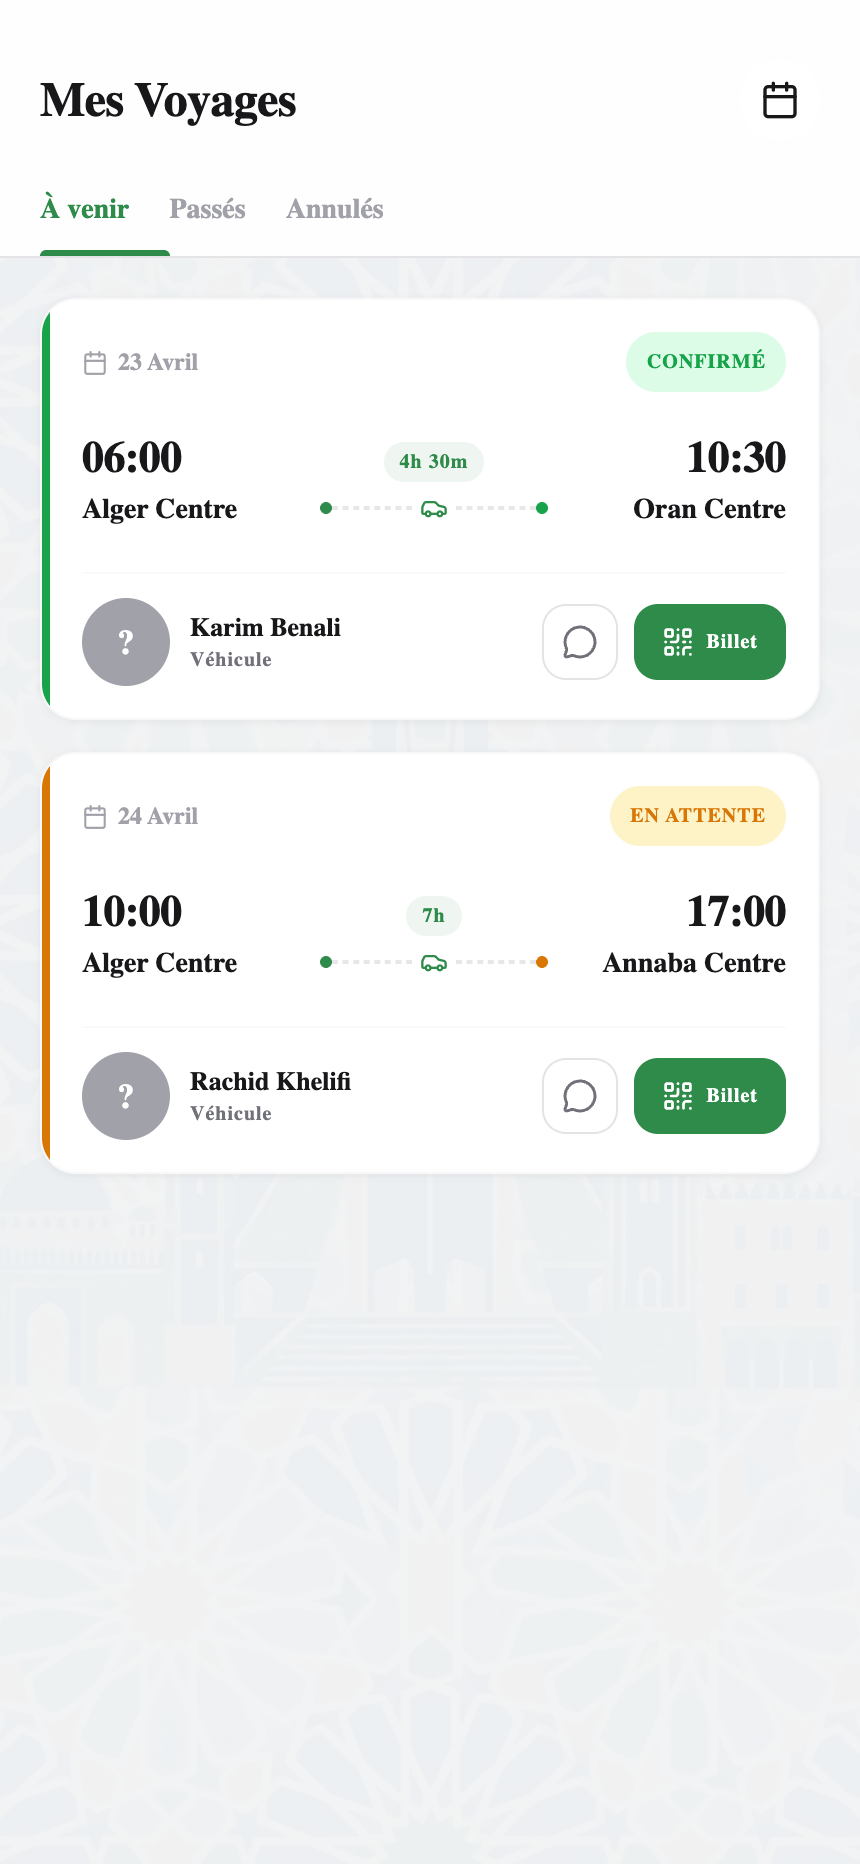
\includegraphics[width=\linewidth]{mobile-all/p_06_trips_upcoming.png}
    {\footnotesize D.6 --- Trajets à venir\par}
\end{minipage}
\end{figure}

\begin{figure}[H]
\centering
\begin{minipage}{0.30\textwidth}
    \centering
    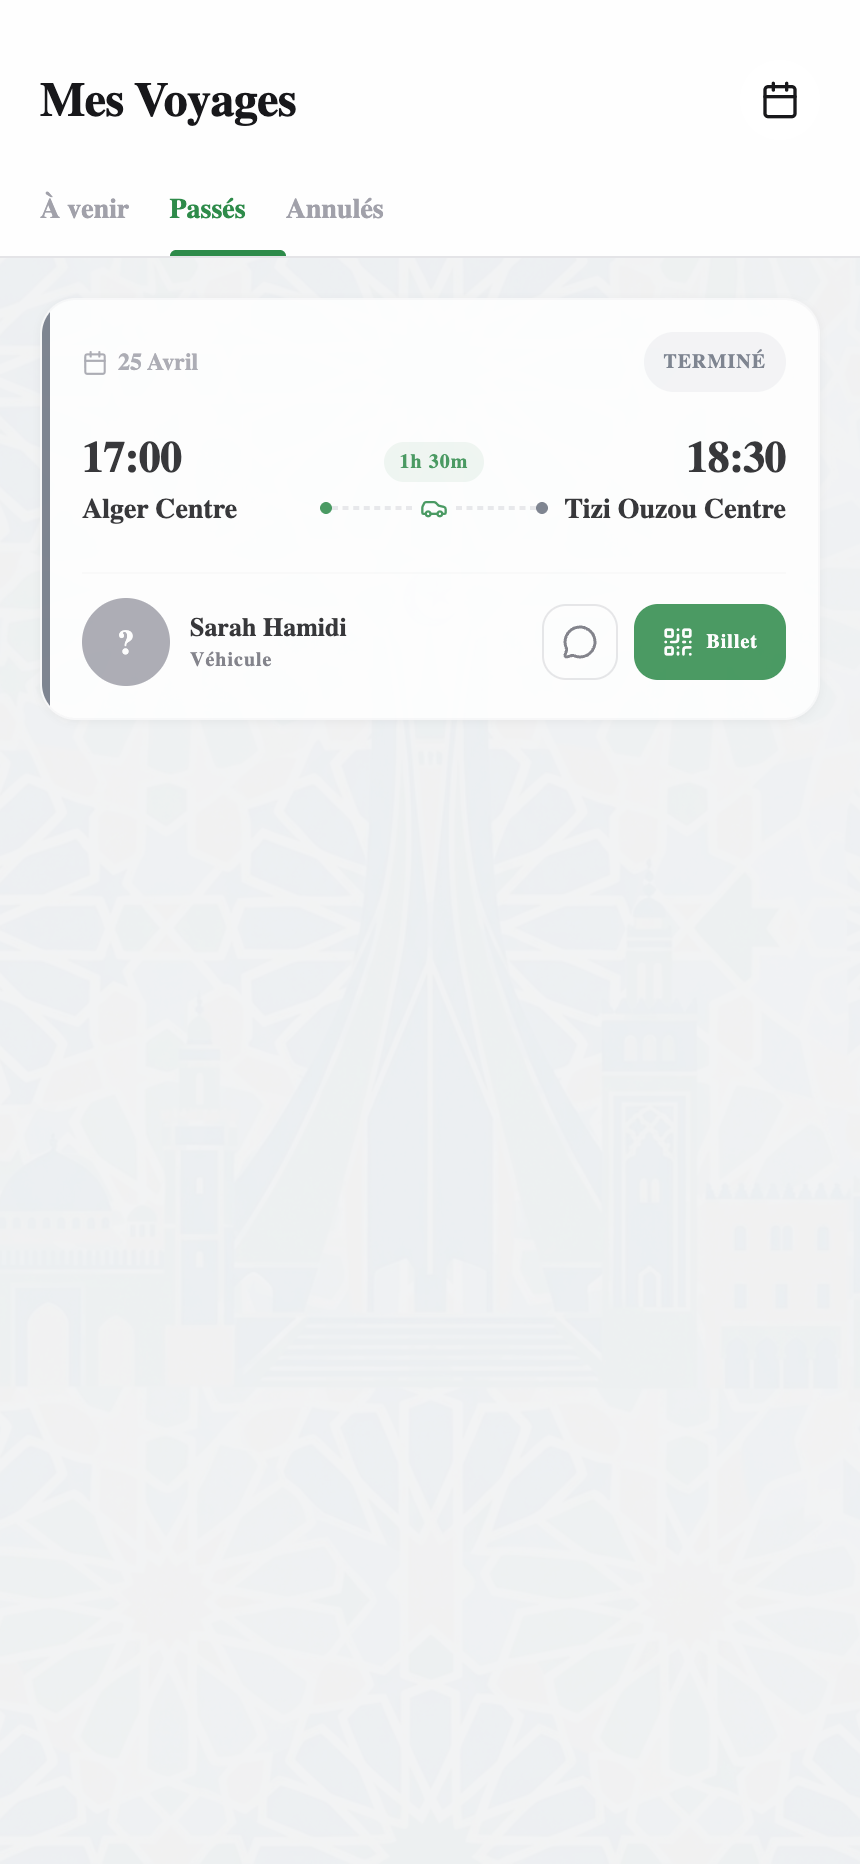
\includegraphics[width=\linewidth]{mobile-all/p_07_trips_past.png}
    {\footnotesize D.7 --- Trajets passés\par}
\end{minipage}\hfill
\begin{minipage}{0.30\textwidth}
    \centering
    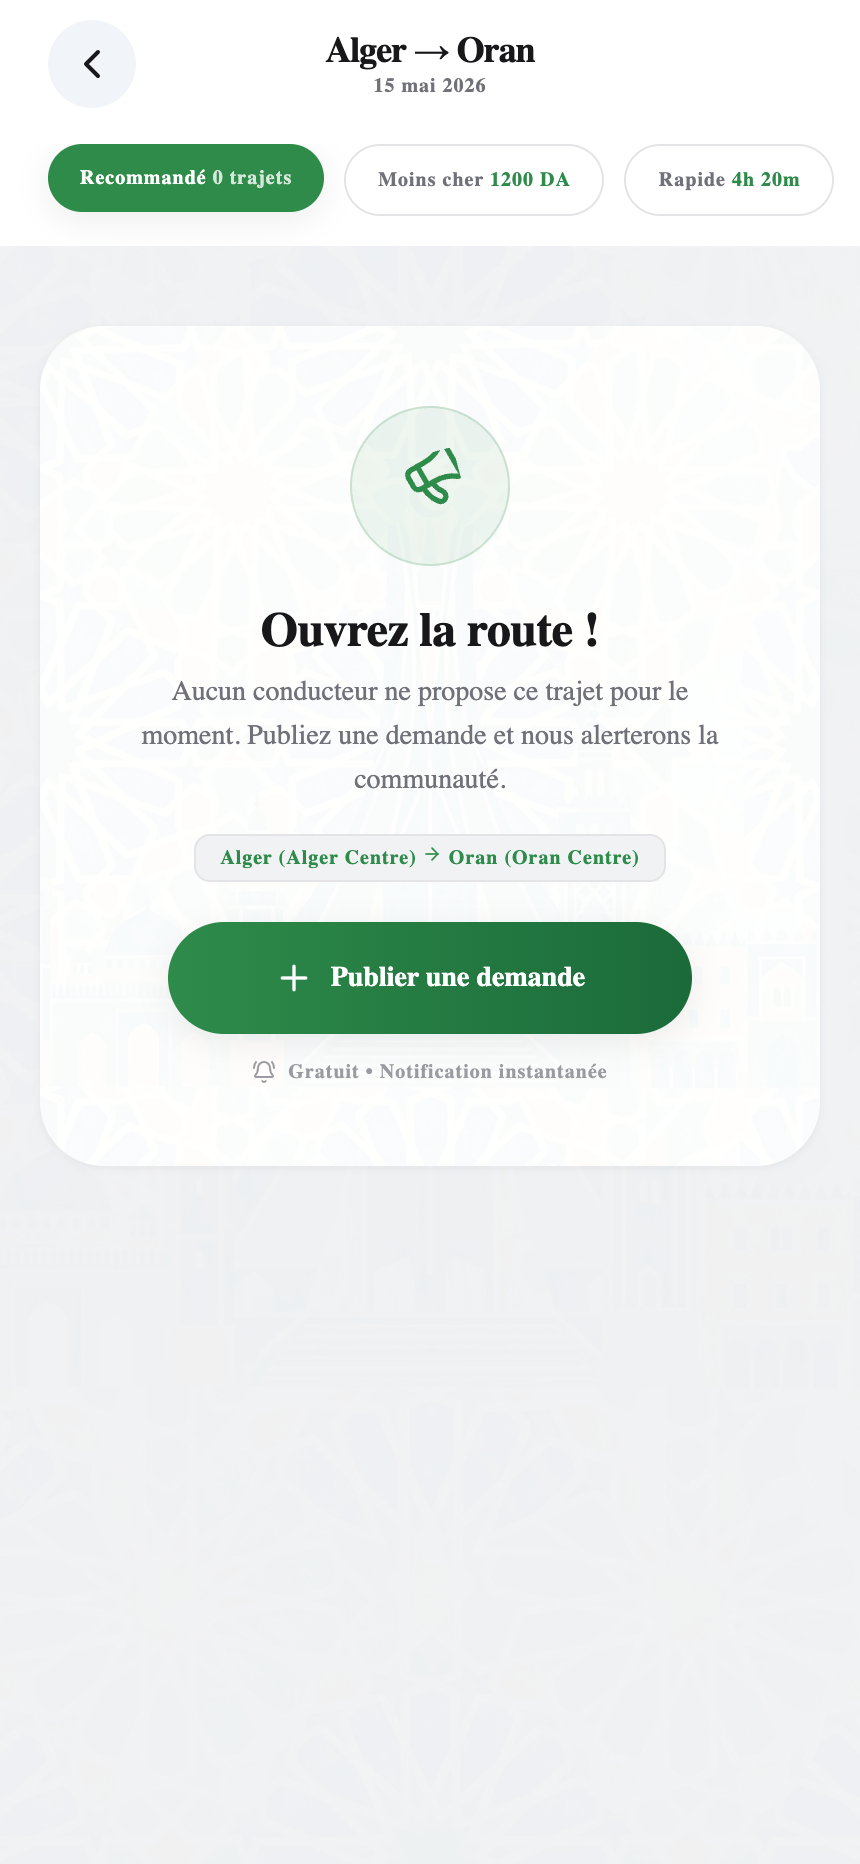
\includegraphics[width=\linewidth]{mobile-all/p_08_search_results.png}
    {\footnotesize D.8 --- Résultats de recherche\par}
\end{minipage}\hfill
\begin{minipage}{0.30\textwidth}
    \centering
    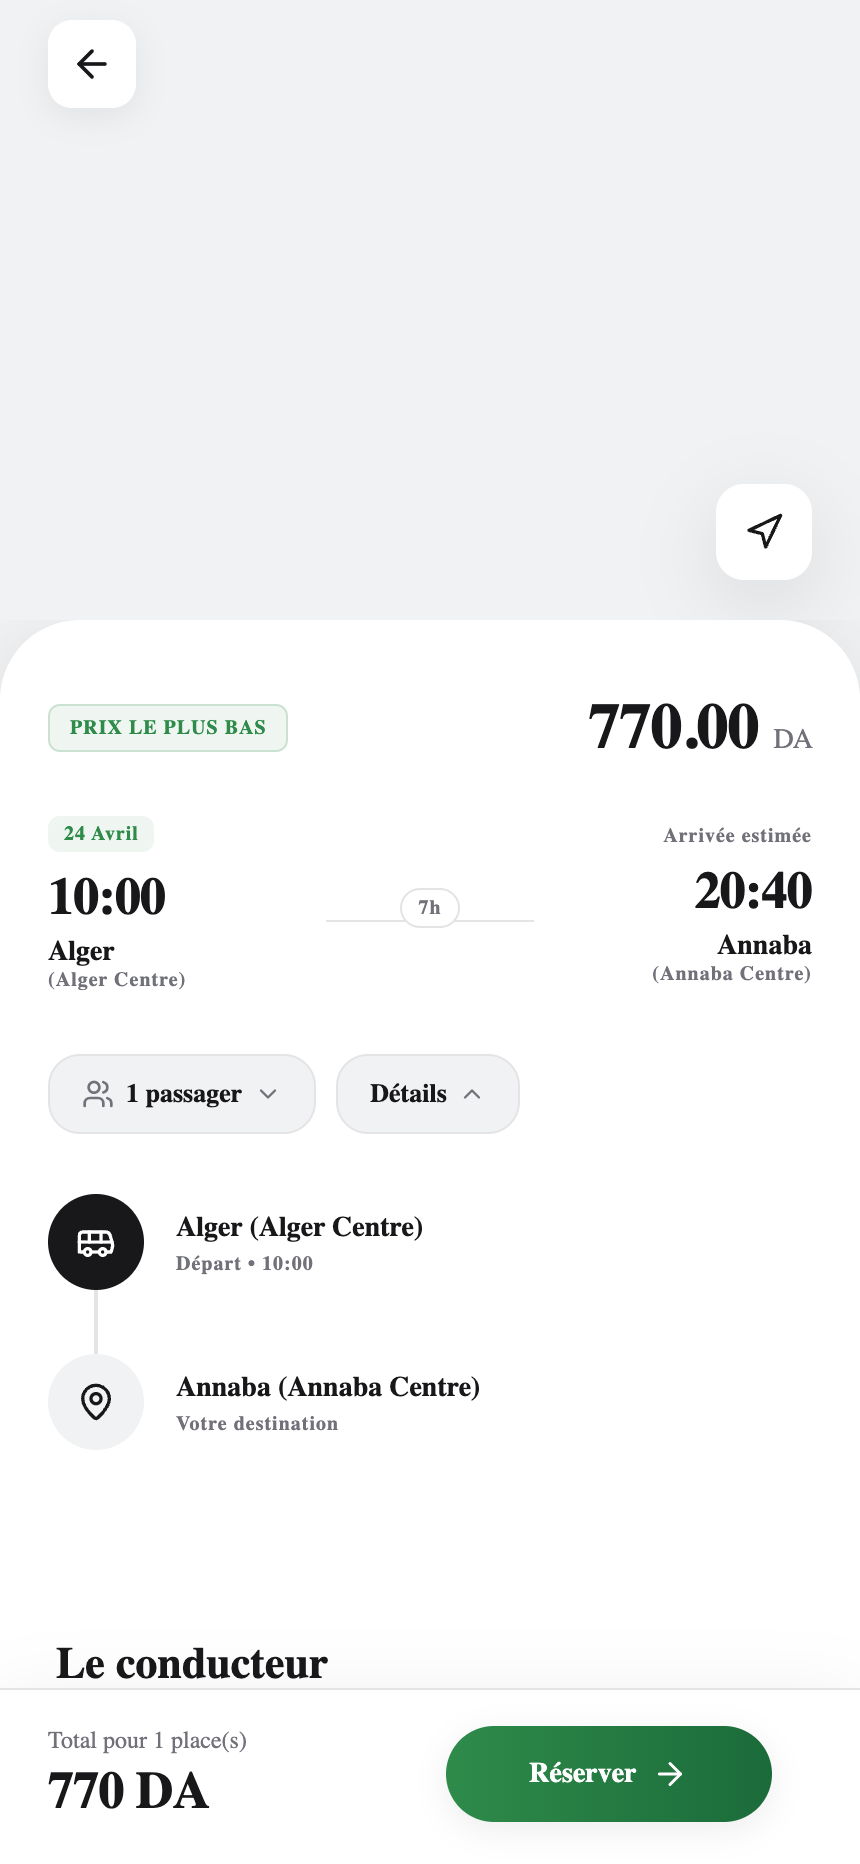
\includegraphics[width=\linewidth]{mobile-all/p_09_trip_details.png}
    {\footnotesize D.9 --- Détail du trajet\par}
\end{minipage}
\end{figure}

\begin{figure}[H]
\centering
\begin{minipage}{0.30\textwidth}
    \centering
    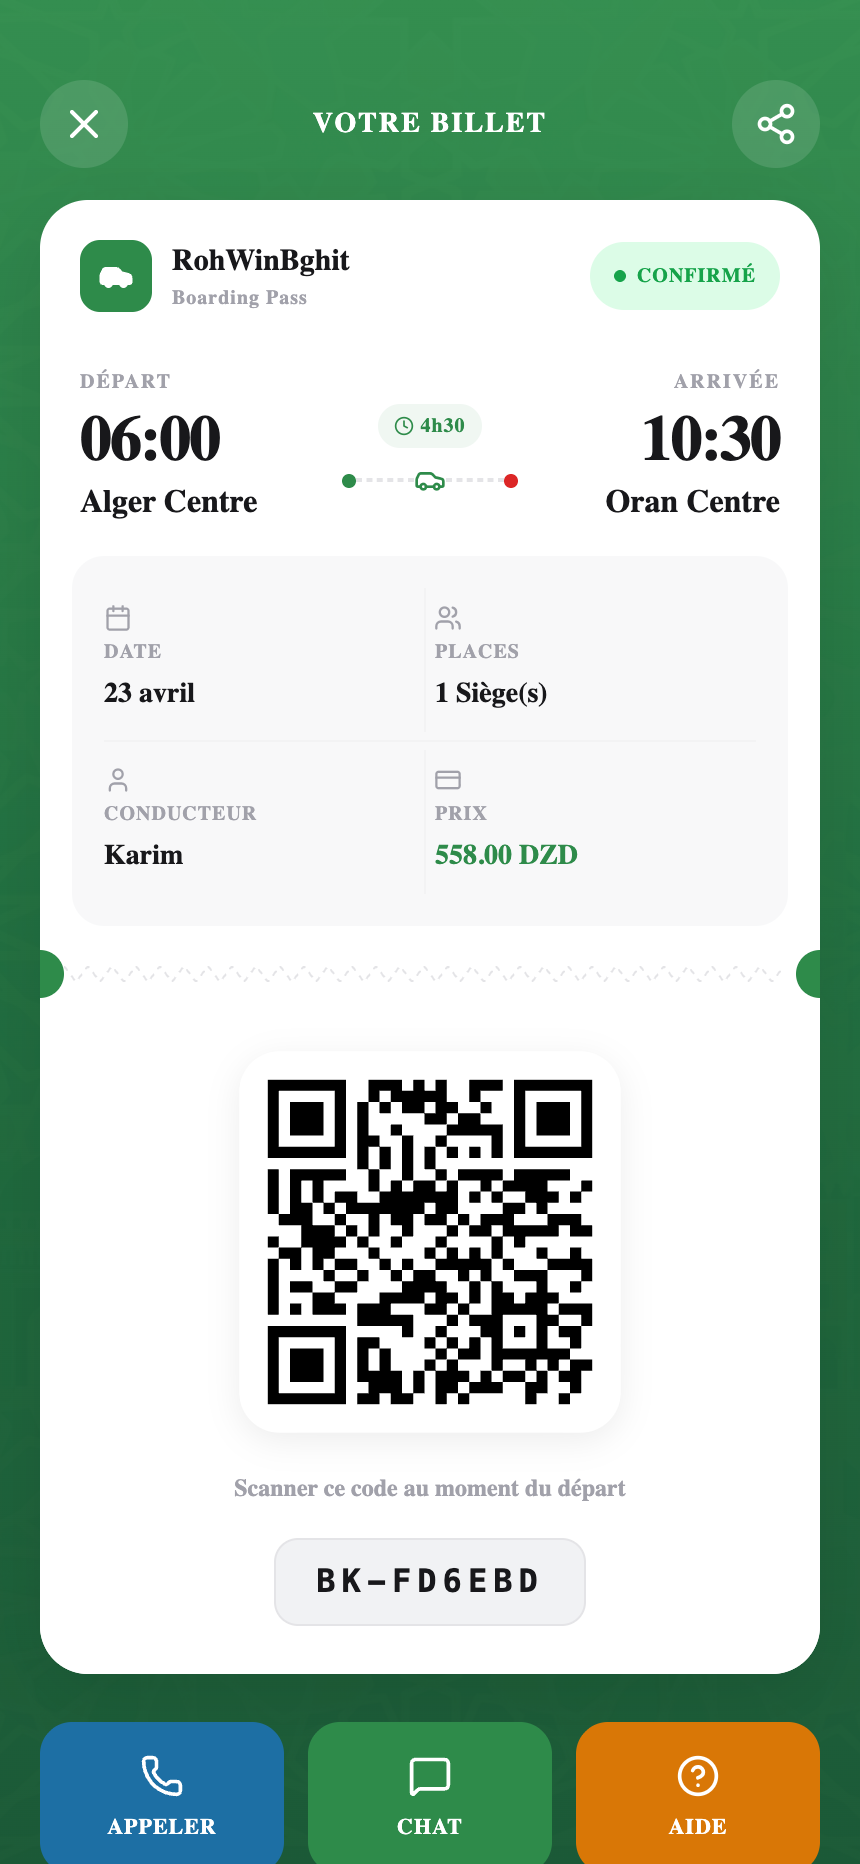
\includegraphics[width=\linewidth]{mobile-all/p_10_ticket.png}
    {\footnotesize D.10 --- Billet numérique\par}
\end{minipage}\hfill
\begin{minipage}{0.30\textwidth}
    \centering
    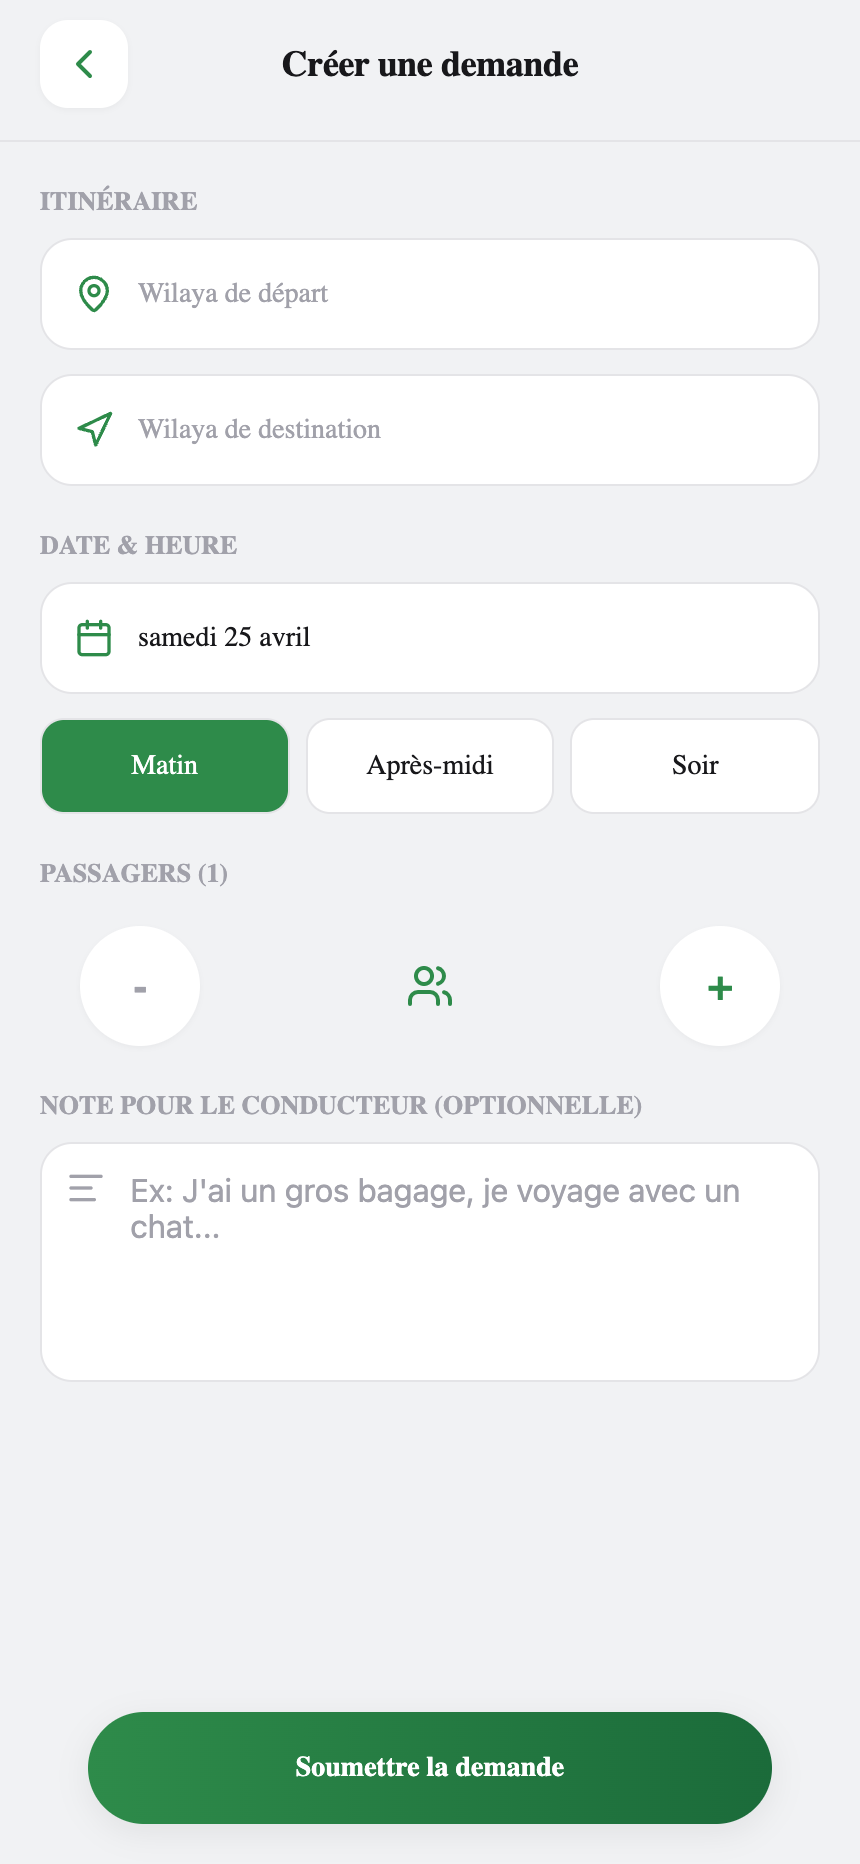
\includegraphics[width=\linewidth]{mobile-all/p_11_create_trip_request.png}
    {\footnotesize D.11 --- Créer demande trajet\par}
\end{minipage}\hfill
\begin{minipage}{0.30\textwidth}
    \centering
    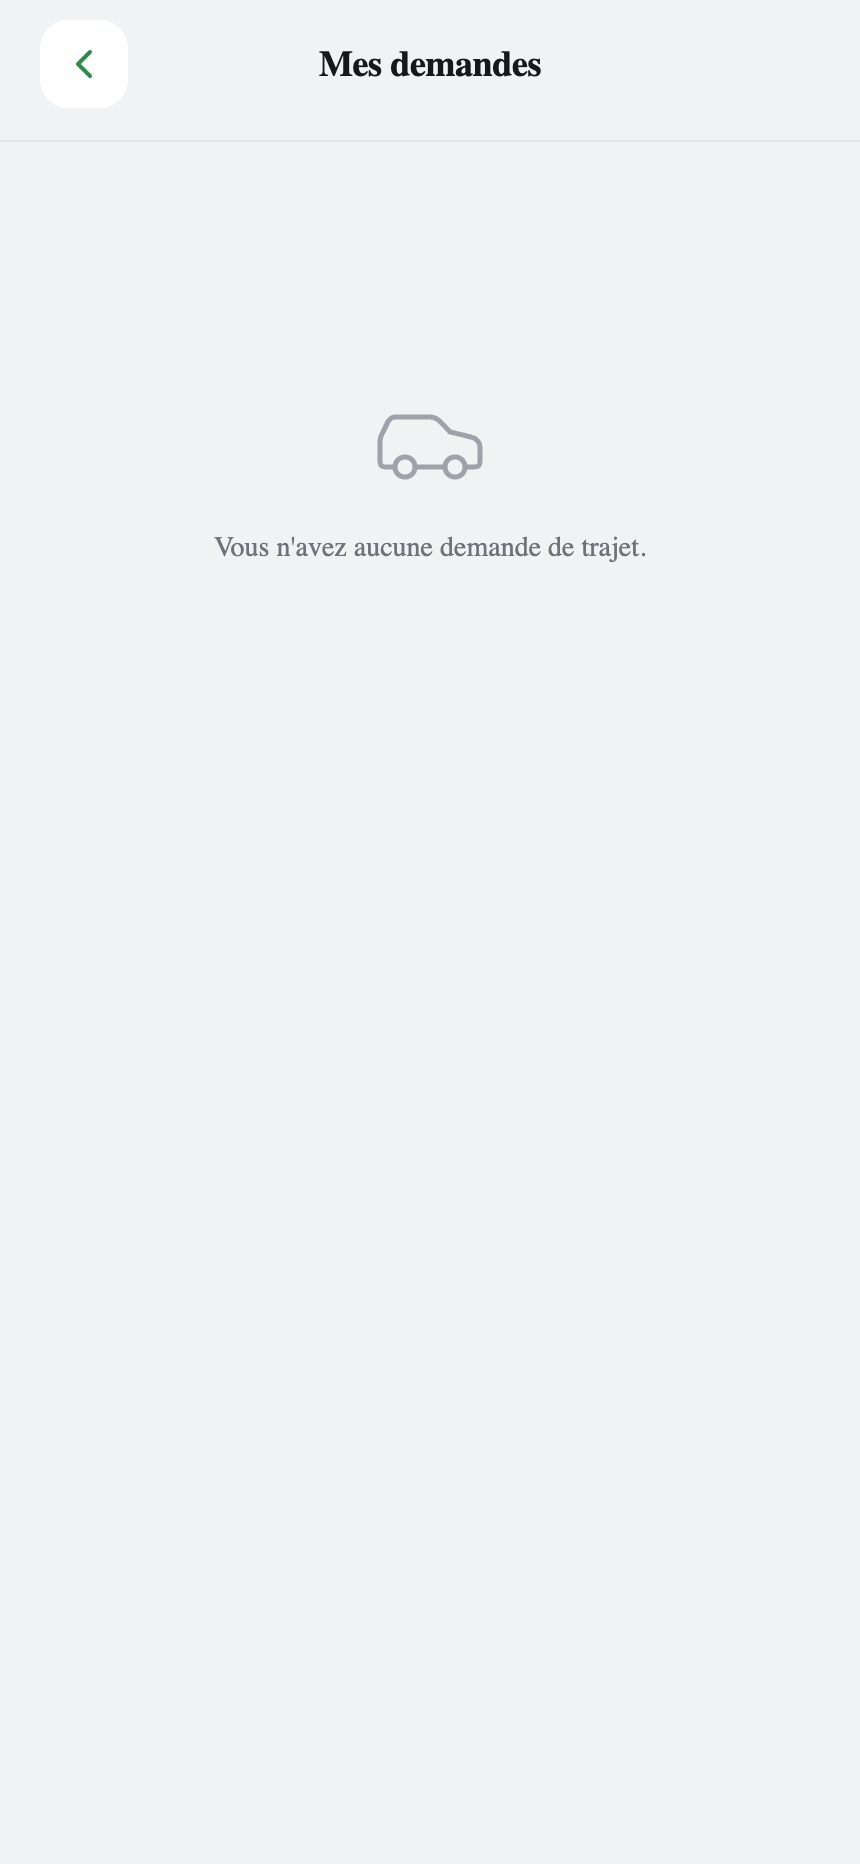
\includegraphics[width=\linewidth]{mobile-all/p_12_my_trip_requests.png}
    {\footnotesize D.12 --- Mes demandes de trajet\par}
\end{minipage}
\end{figure}

\begin{figure}[H]
\centering
\begin{minipage}{0.30\textwidth}
    \centering
    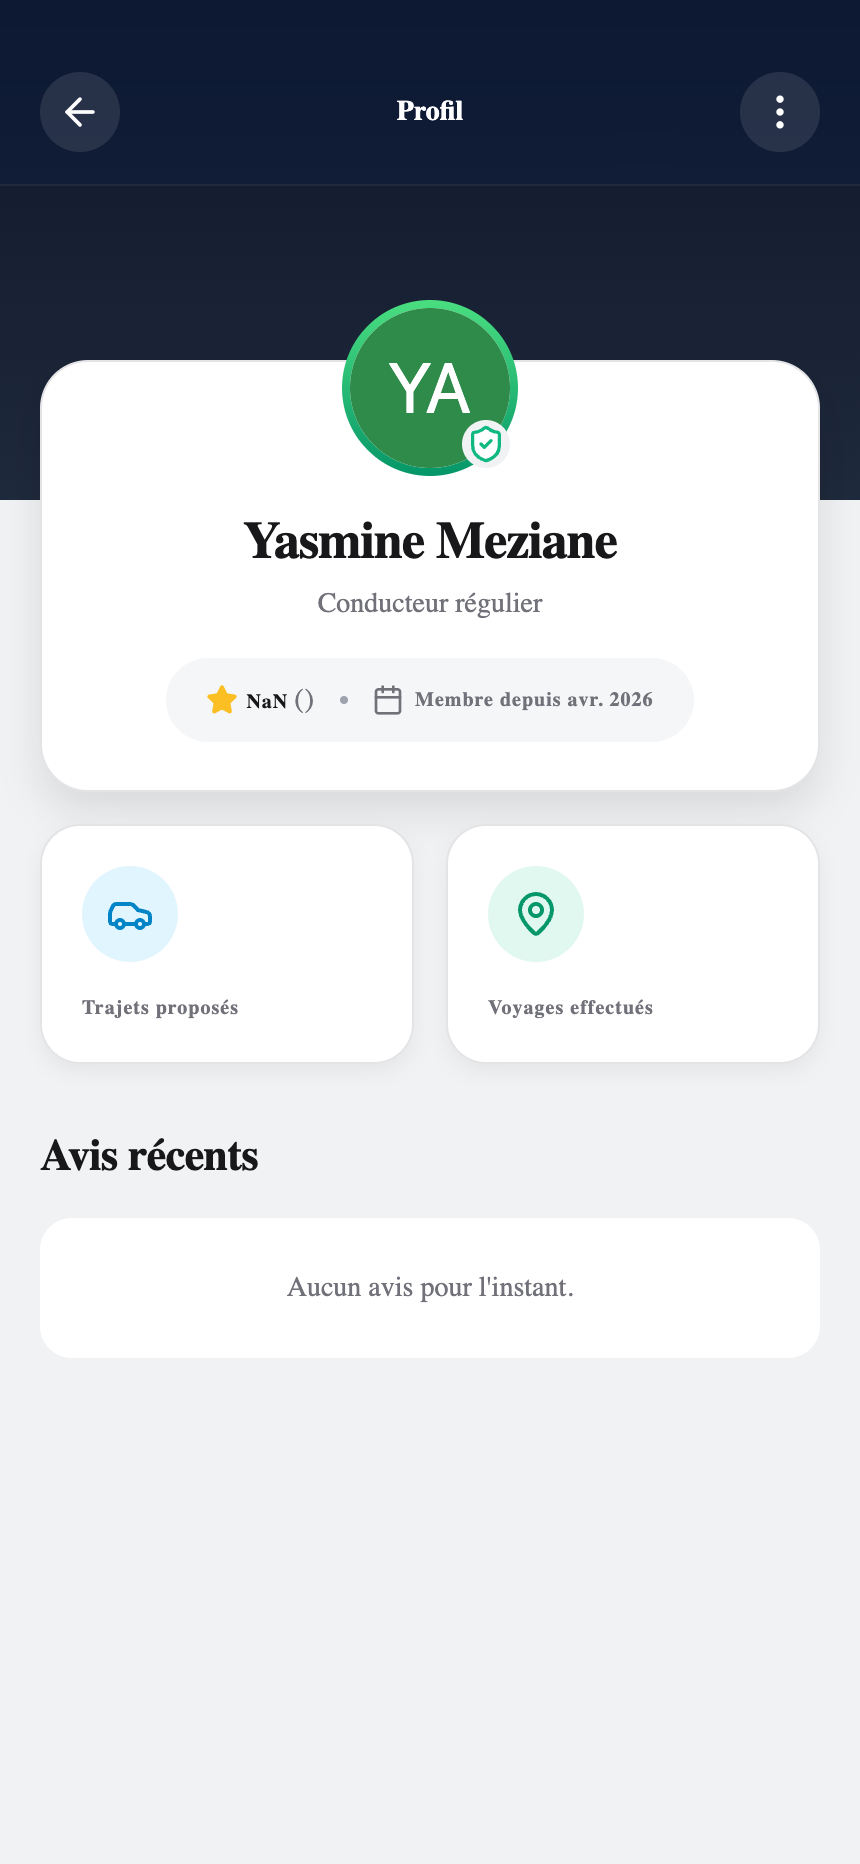
\includegraphics[width=\linewidth]{mobile-all/p_13_public_profile.png}
    {\footnotesize D.13 --- Profil public\par}
\end{minipage}\hfill
\begin{minipage}{0.30\textwidth}
    \centering
    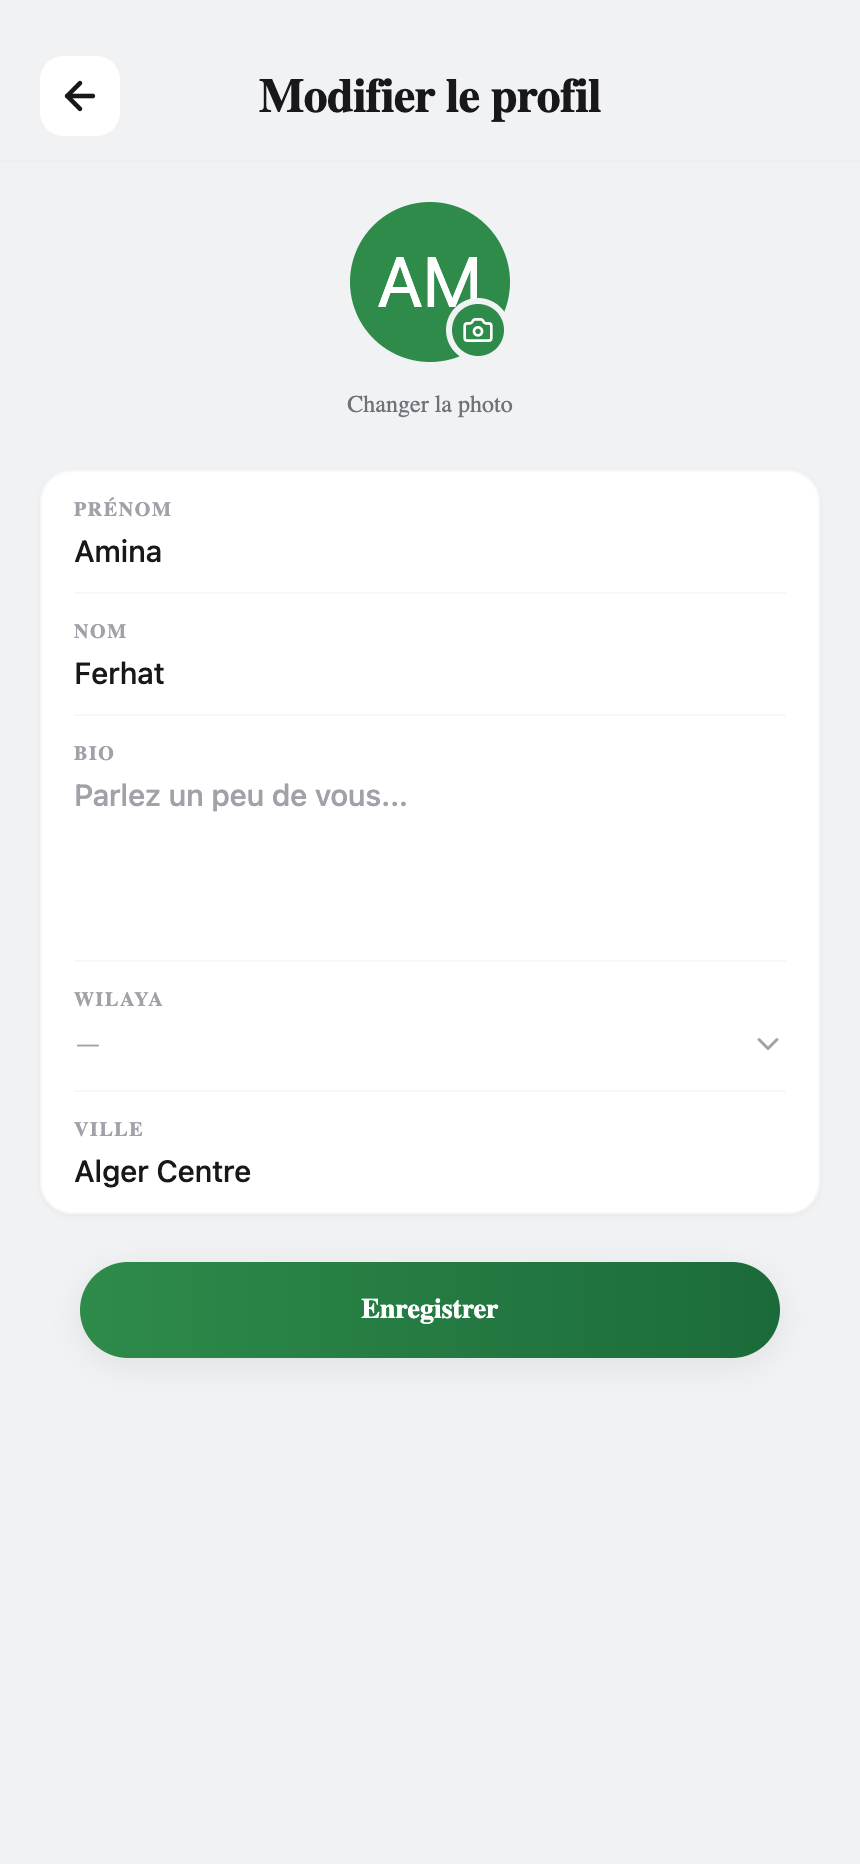
\includegraphics[width=\linewidth]{mobile-all/p_14_edit_profile.png}
    {\footnotesize D.14 --- Modifier profil\par}
\end{minipage}\hfill
\begin{minipage}{0.30\textwidth}
    \centering
    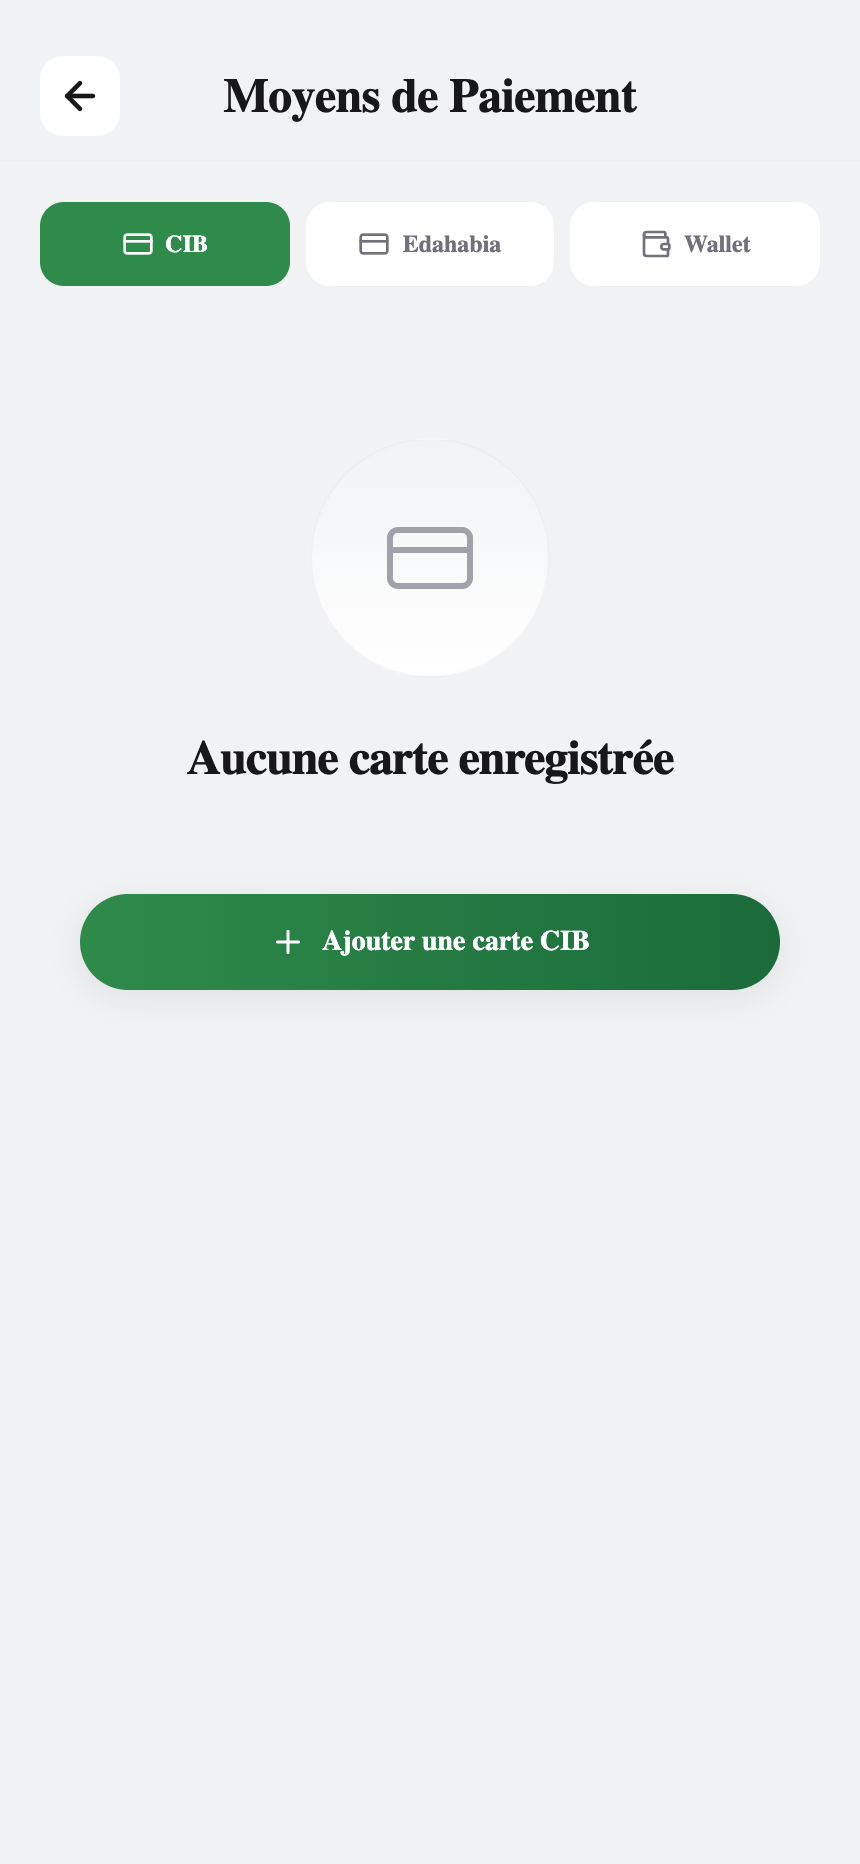
\includegraphics[width=\linewidth]{mobile-all/p_15_payment_methods.png}
    {\footnotesize D.15 --- Méthodes de paiement\par}
\end{minipage}
\end{figure}

\begin{figure}[H]
\centering
\begin{minipage}{0.30\textwidth}
    \centering
    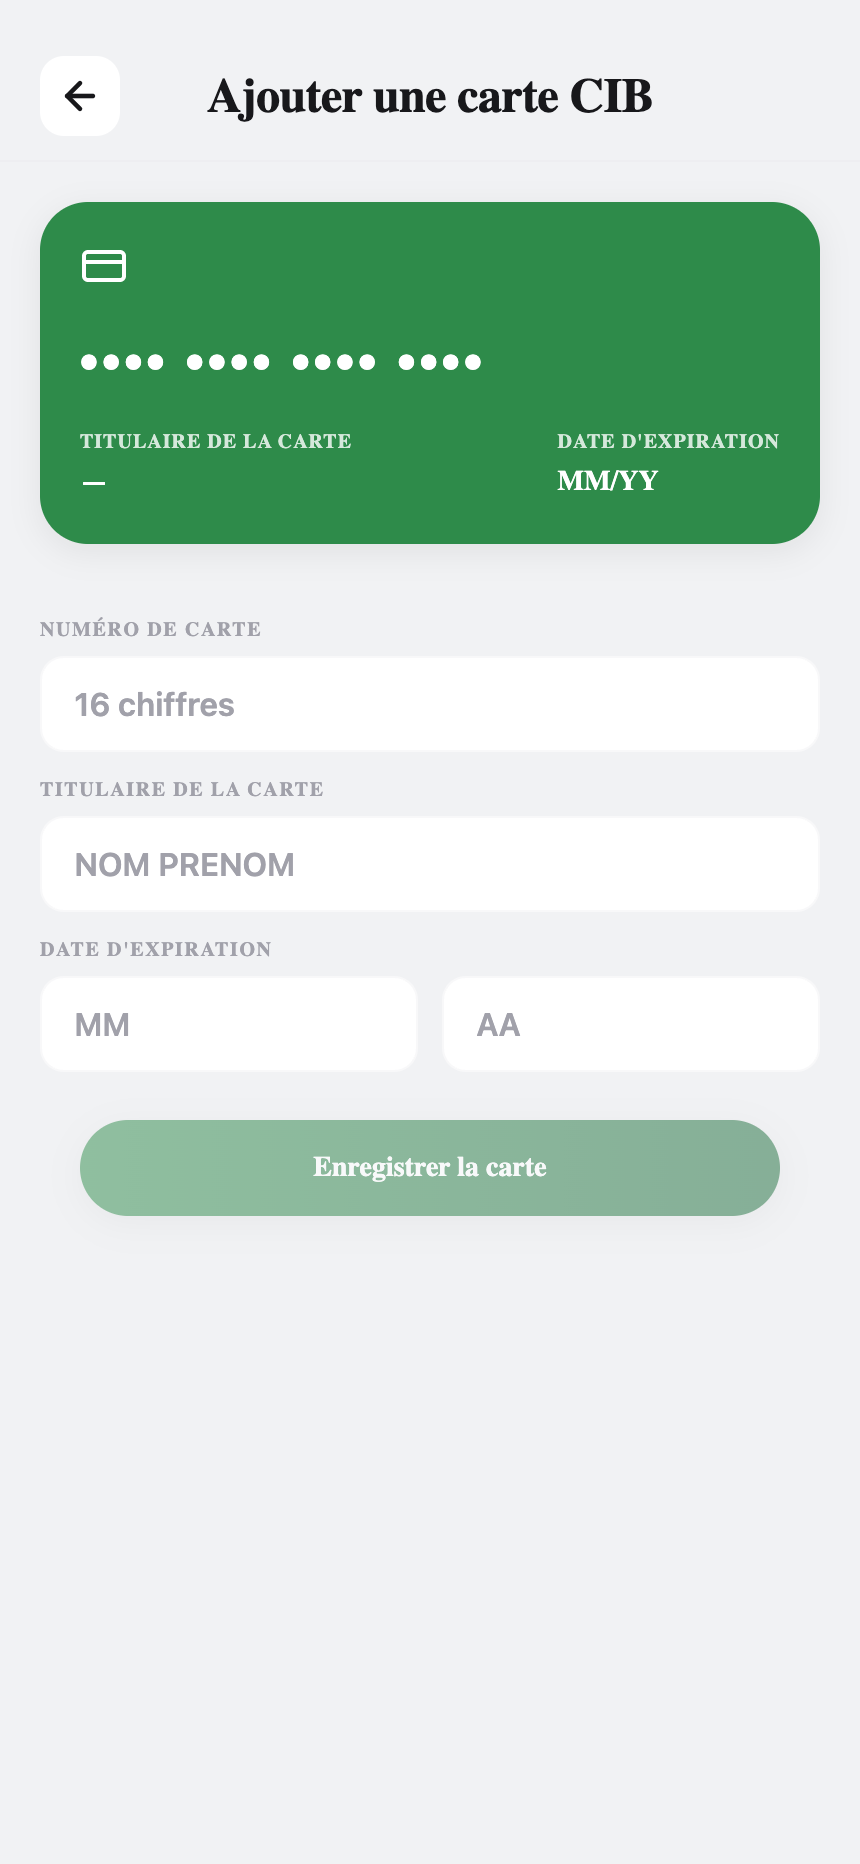
\includegraphics[width=\linewidth]{mobile-all/p_16_add_card.png}
    {\footnotesize D.16 --- Ajout carte bancaire\par}
\end{minipage}\hfill
\begin{minipage}{0.30\textwidth}
    \centering
    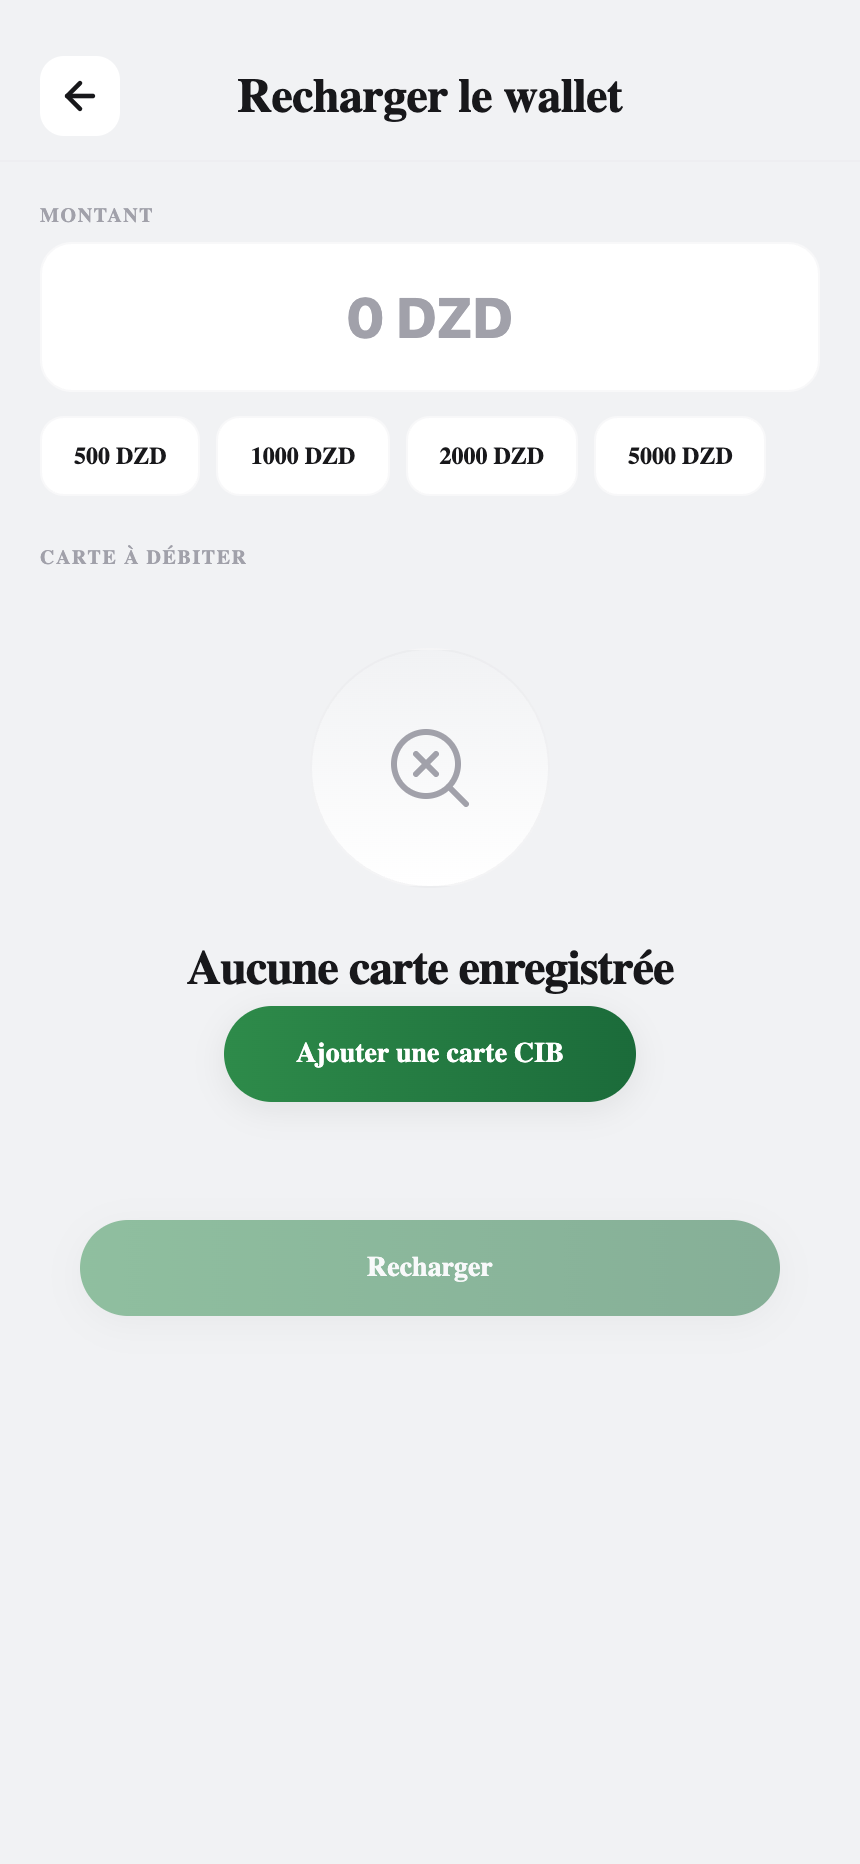
\includegraphics[width=\linewidth]{mobile-all/p_17_wallet_recharge.png}
    {\footnotesize D.17 --- Recharge portefeuille\par}
\end{minipage}\hfill
\begin{minipage}{0.30\textwidth}
    \centering
    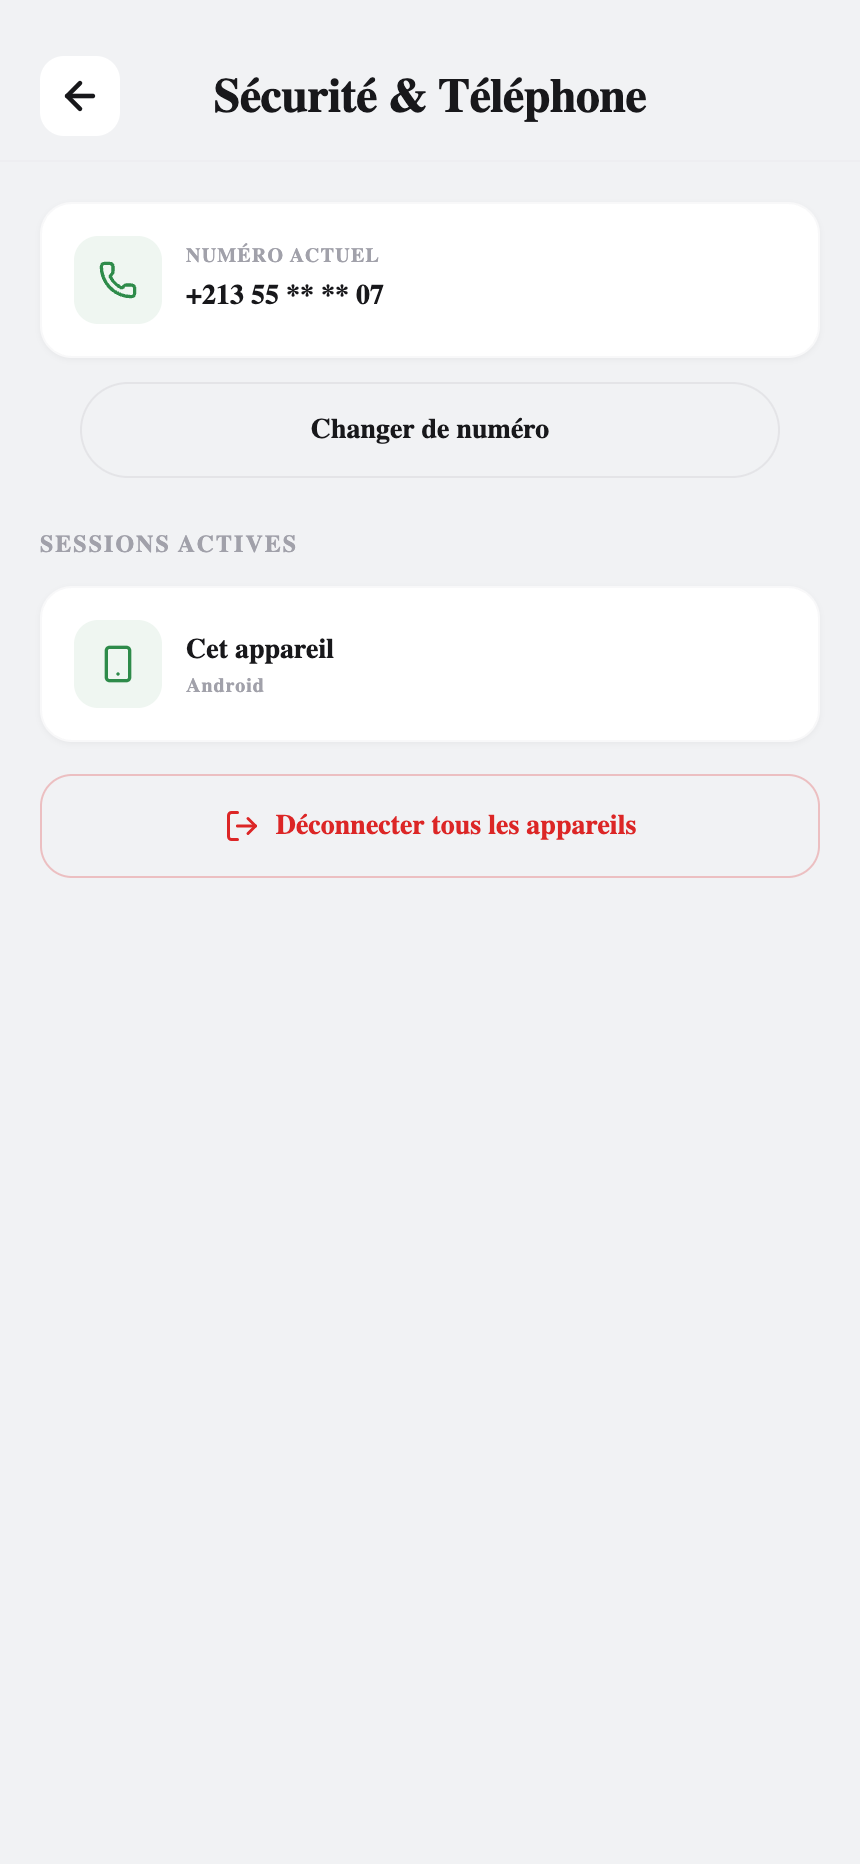
\includegraphics[width=\linewidth]{mobile-all/p_18_security_phone.png}
    {\footnotesize D.18 --- Sécurité du compte\par}
\end{minipage}
\end{figure}

\begin{figure}[H]
\centering
\begin{minipage}{0.30\textwidth}
    \centering
    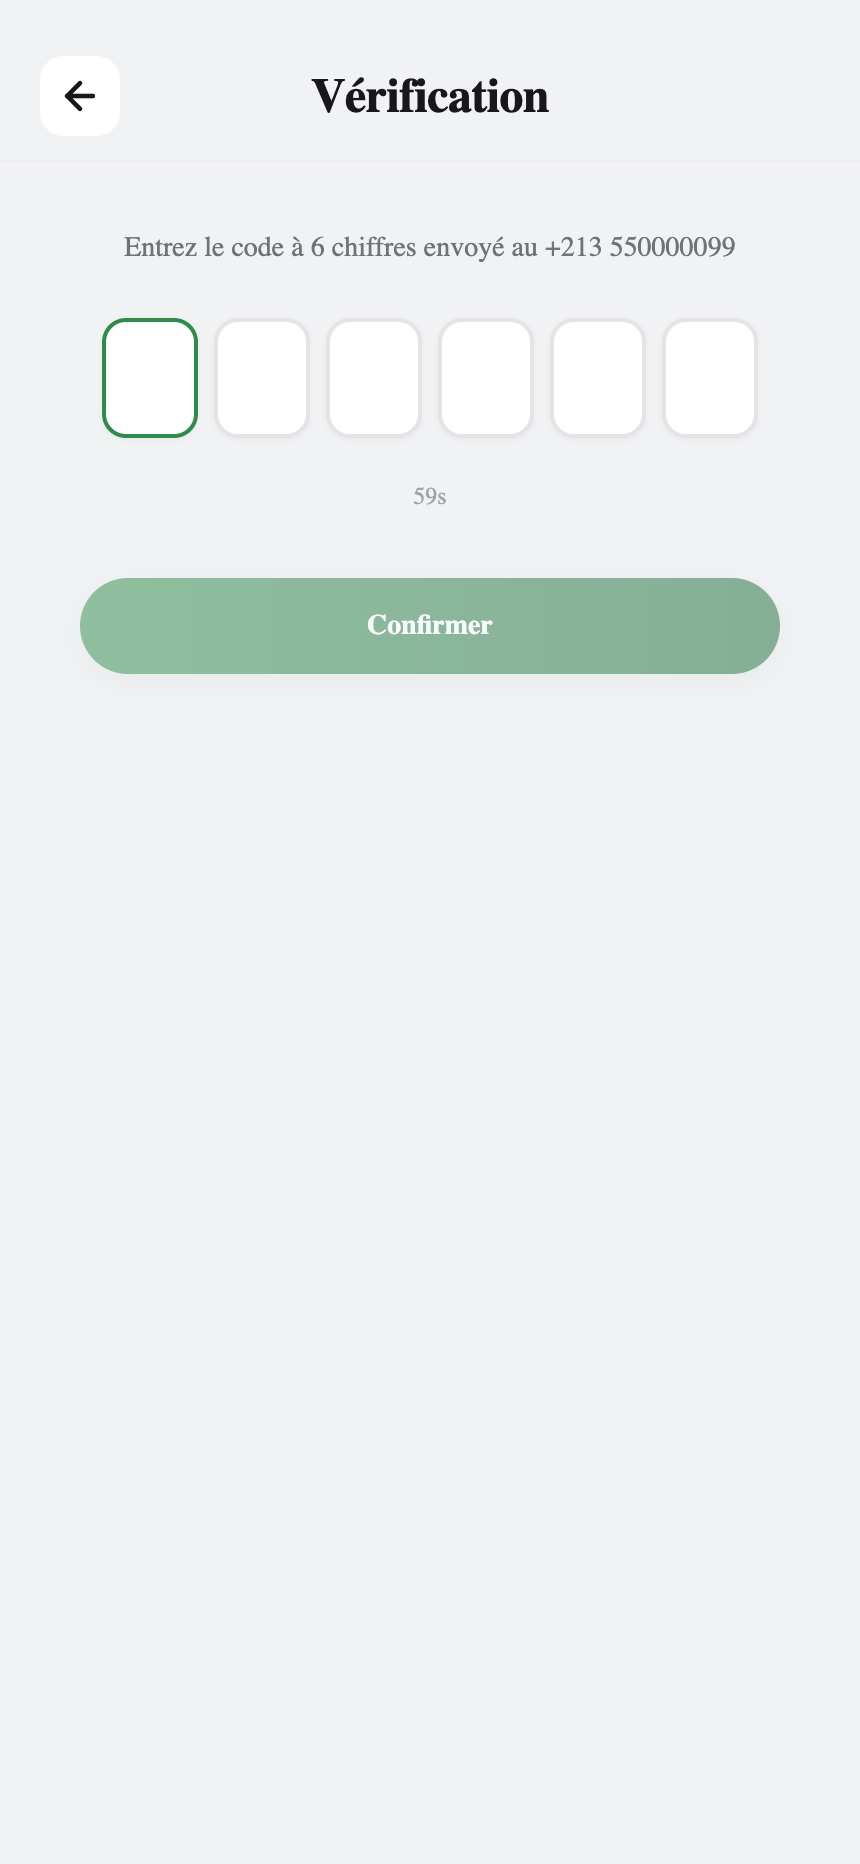
\includegraphics[width=\linewidth]{mobile-all/p_19_change_phone_otp.png}
    {\footnotesize D.19 --- Changement numéro OTP\par}
\end{minipage}\hfill
\begin{minipage}{0.30\textwidth}
    \centering
    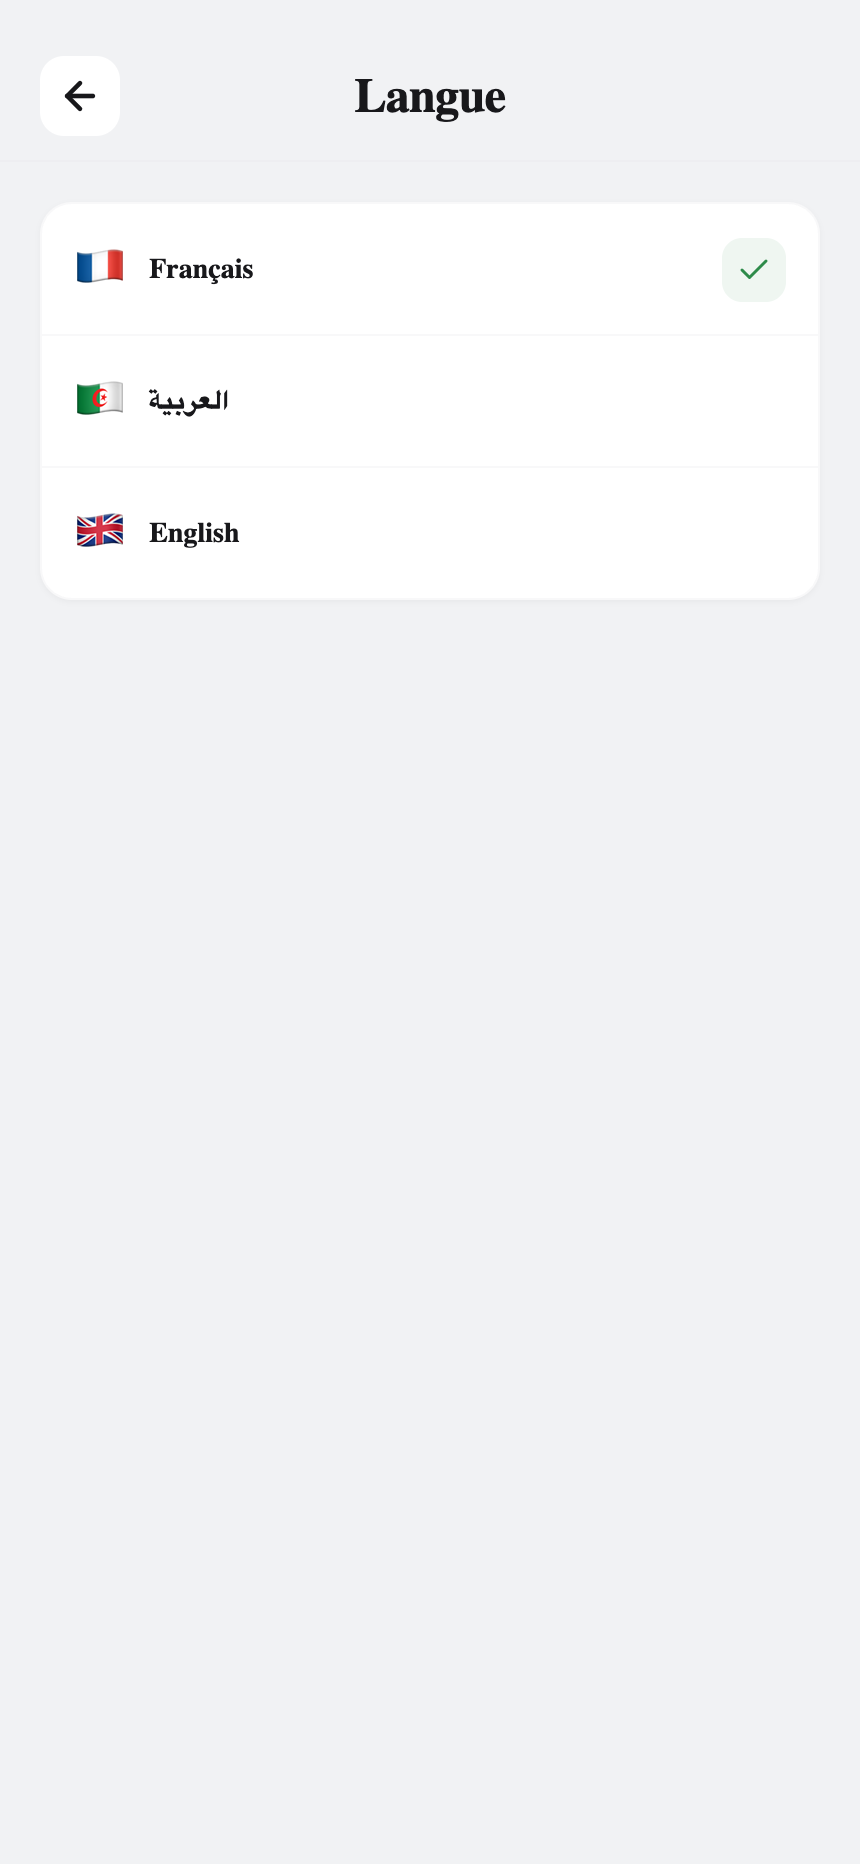
\includegraphics[width=\linewidth]{mobile-all/p_20_language_select.png}
    {\footnotesize D.20 --- Sélection langue\par}
\end{minipage}\hfill
\begin{minipage}{0.30\textwidth}
    \centering
    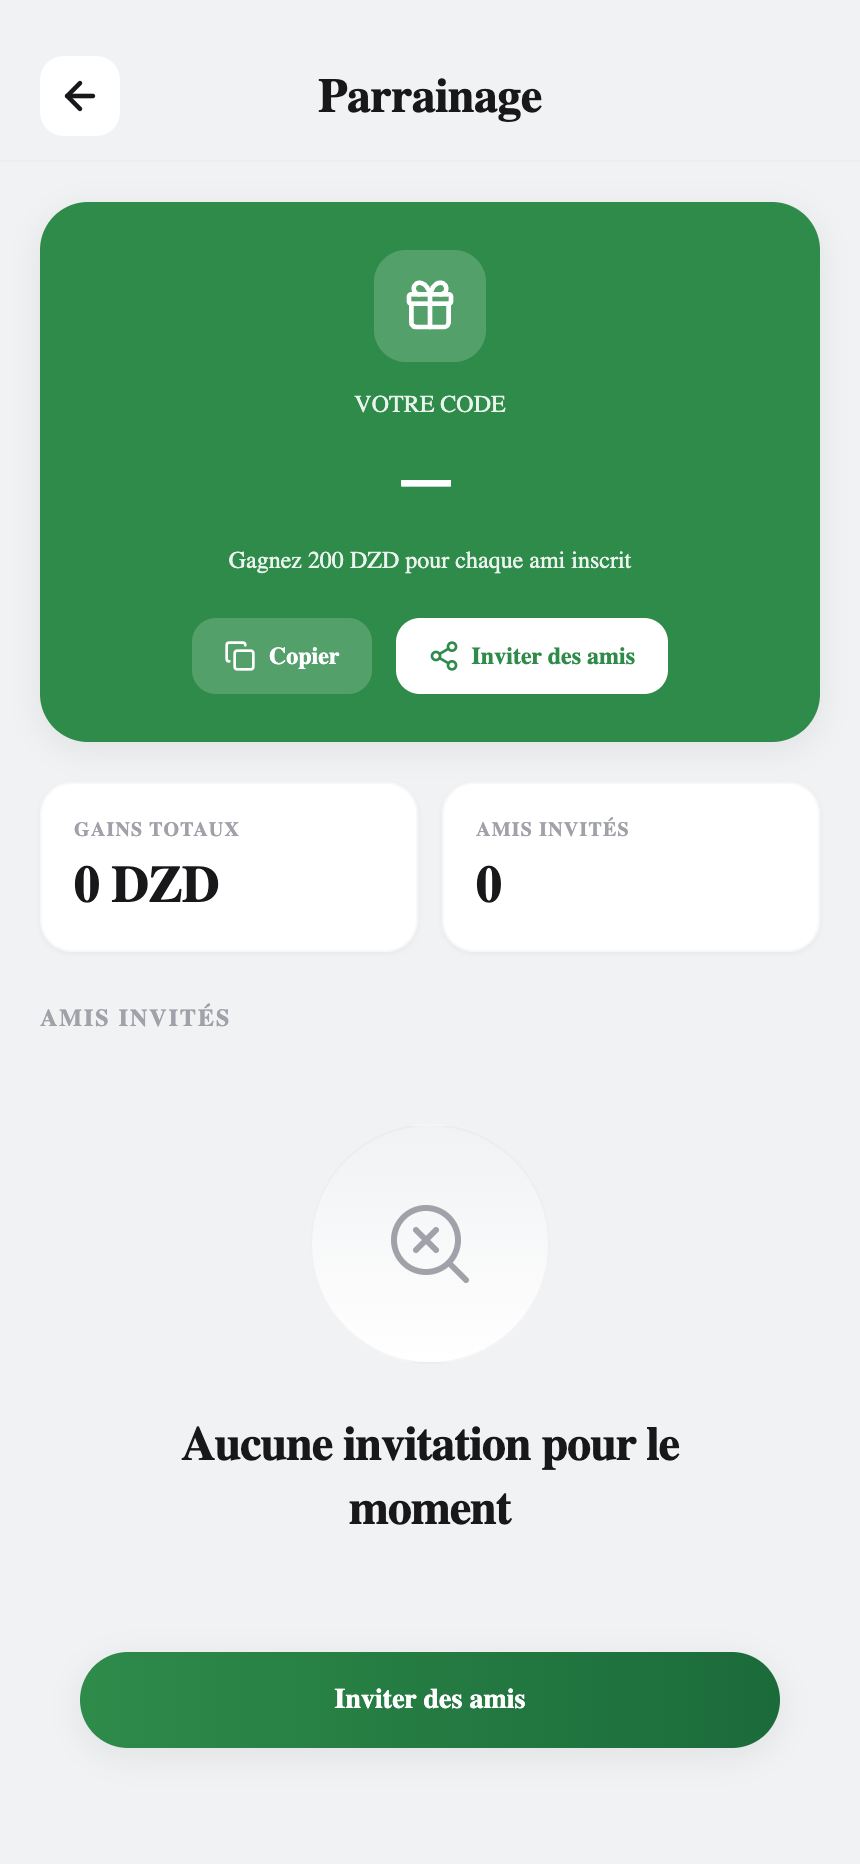
\includegraphics[width=\linewidth]{mobile-all/p_21_referral.png}
    {\footnotesize D.21 --- Parrainage\par}
\end{minipage}
\end{figure}

\begin{figure}[H]
\centering
\begin{minipage}{0.30\textwidth}
    \centering
    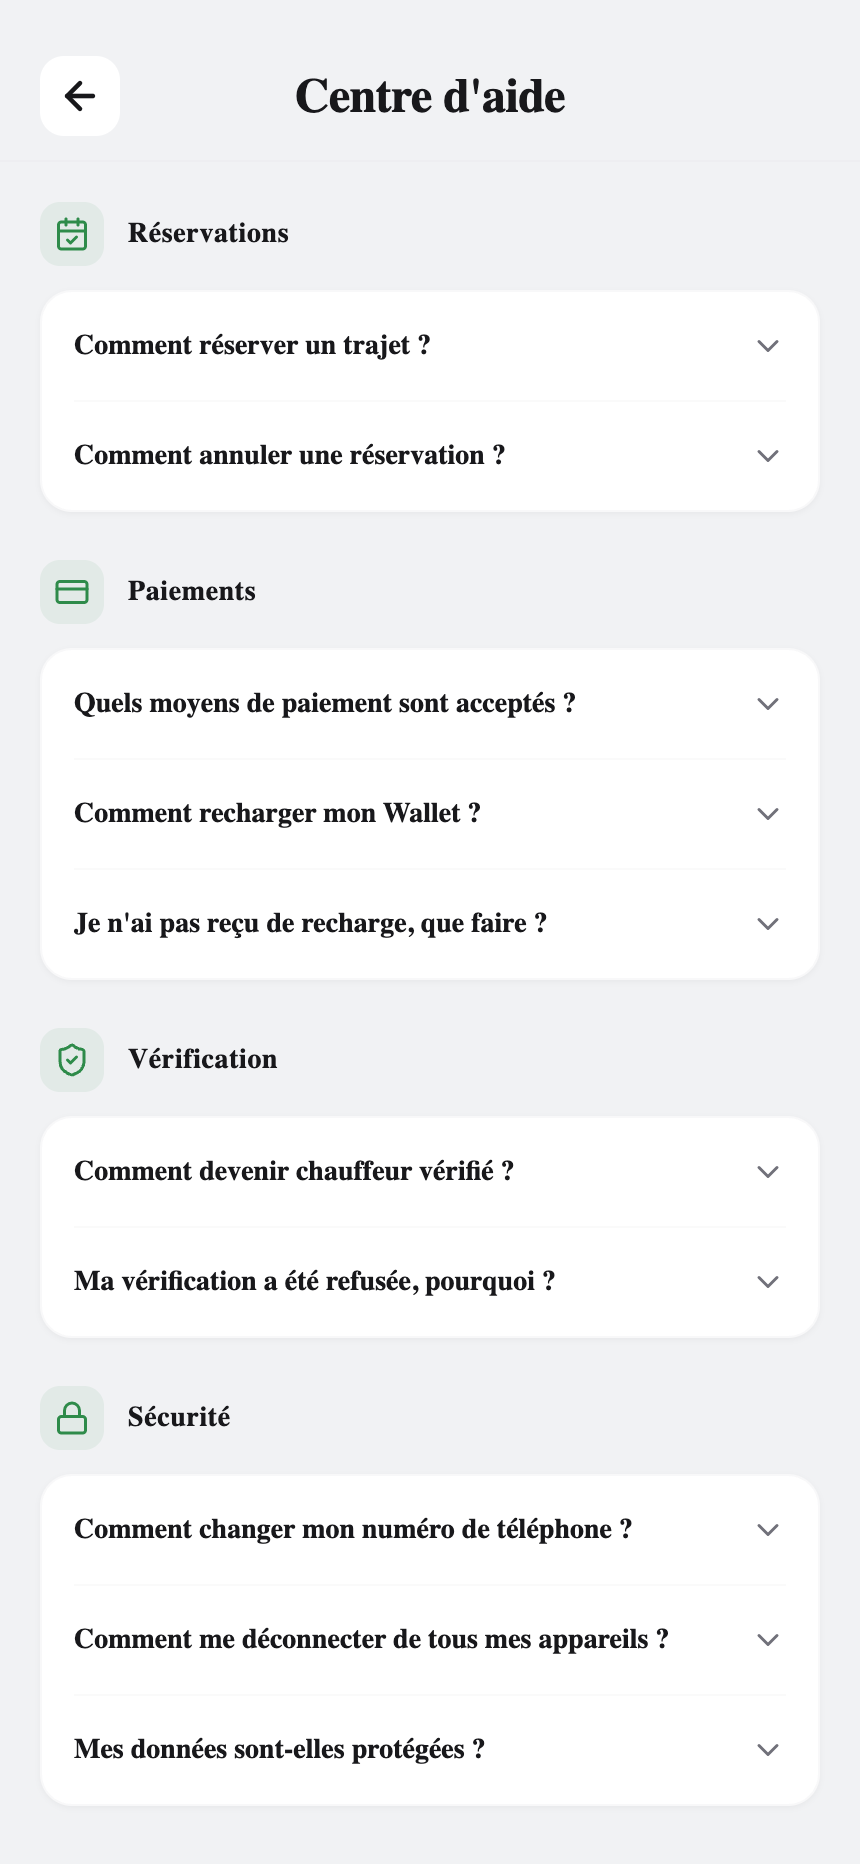
\includegraphics[width=\linewidth]{mobile-all/p_22_help_center.png}
    {\footnotesize D.22 --- Centre d'aide\par}
\end{minipage}\hfill
\begin{minipage}{0.30\textwidth}
    \centering
    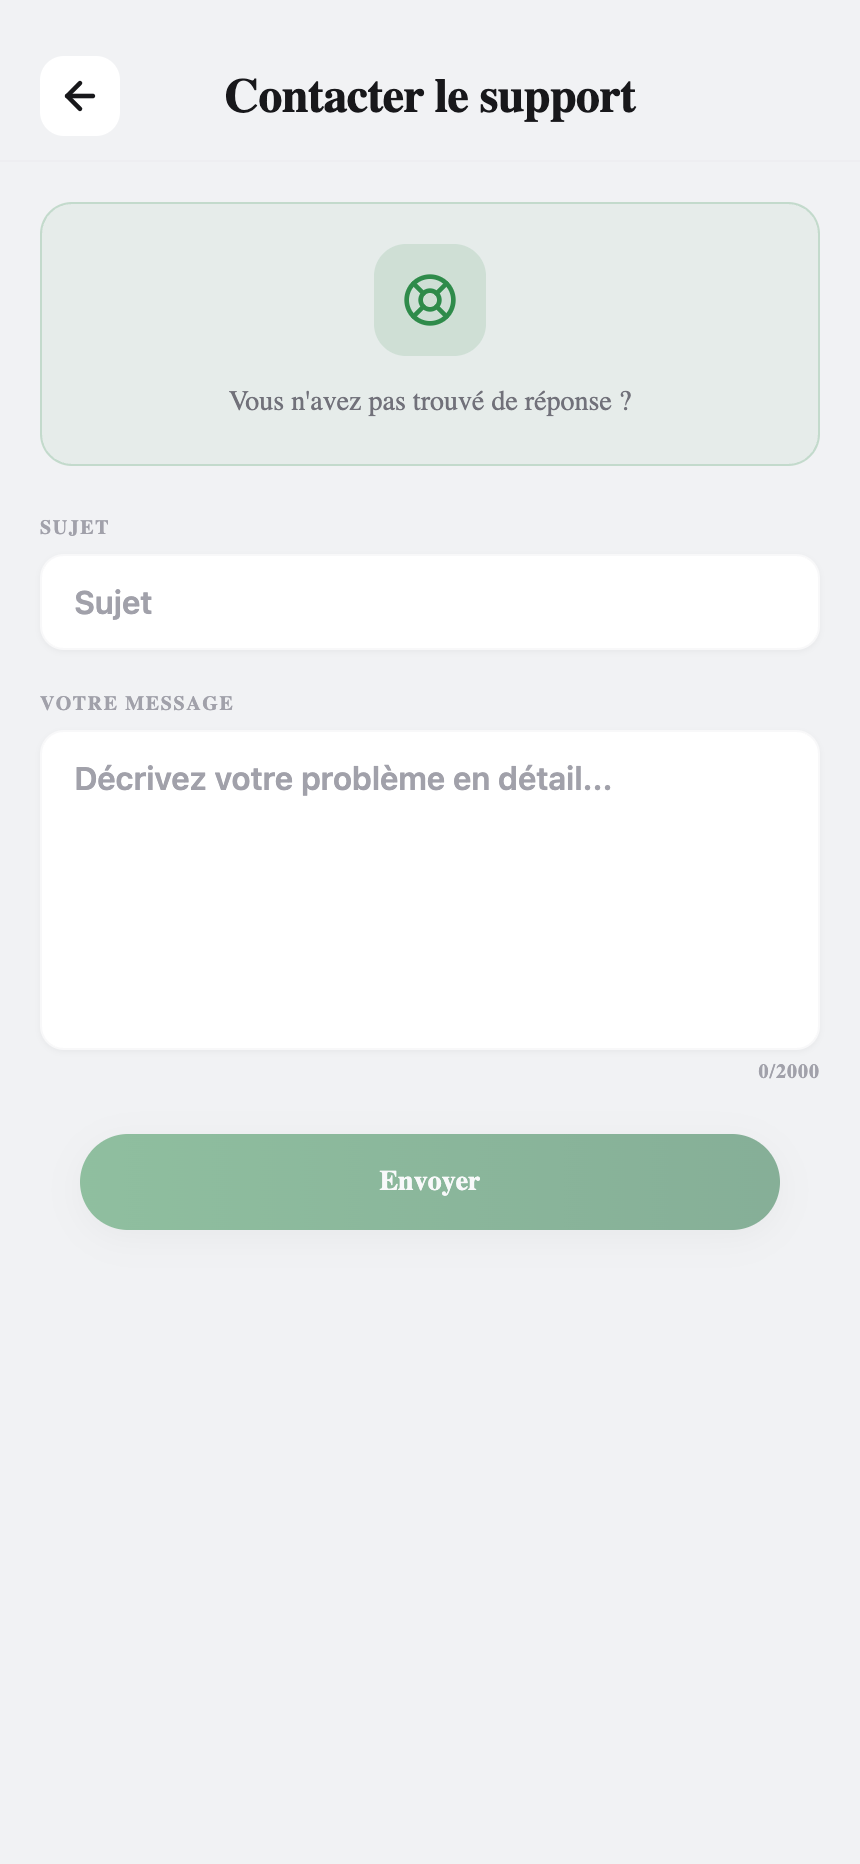
\includegraphics[width=\linewidth]{mobile-all/p_23_contact_support.png}
    {\footnotesize D.23 --- Contacter le support\par}
\end{minipage}\hfill
\begin{minipage}{0.30\textwidth}
    \centering
    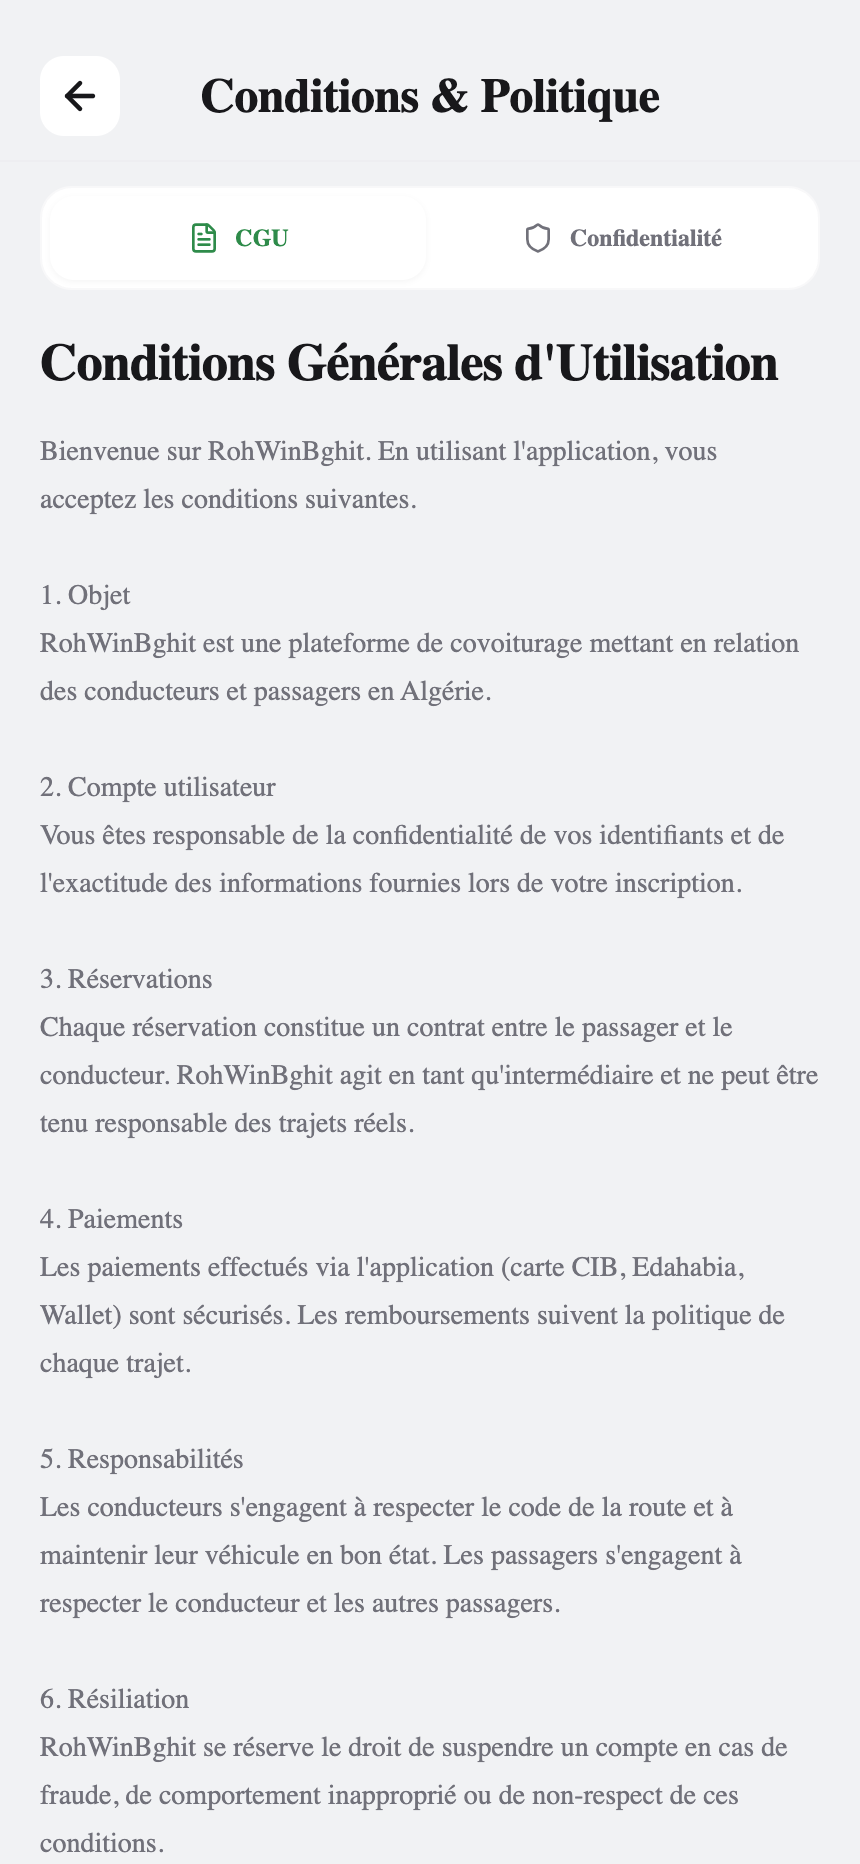
\includegraphics[width=\linewidth]{mobile-all/p_24_terms_legal.png}
    {\footnotesize D.24 --- CGU et confidentialité\par}
\end{minipage}
\end{figure}

\begin{figure}[H]
\centering
\begin{minipage}{0.30\textwidth}
    \centering
    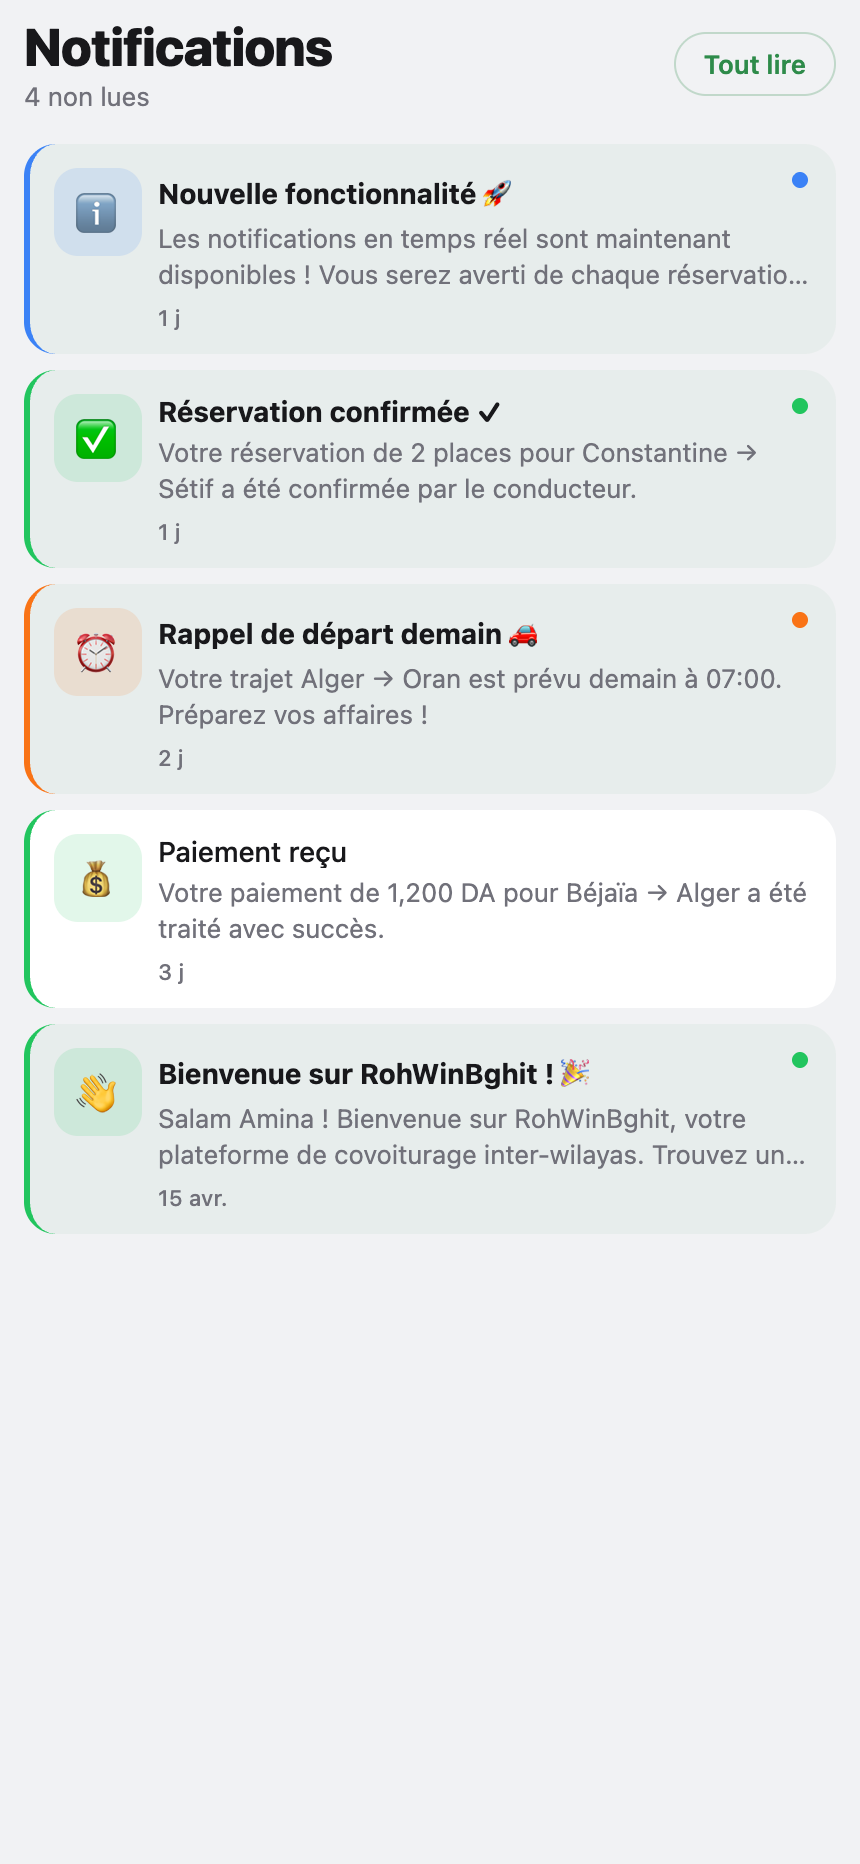
\includegraphics[width=\linewidth]{mobile-all/p_25_notifications.png}
    {\footnotesize D.25 --- Préf. notifications\par}
\end{minipage}\hfill
\begin{minipage}{0.30\textwidth}
    \centering
    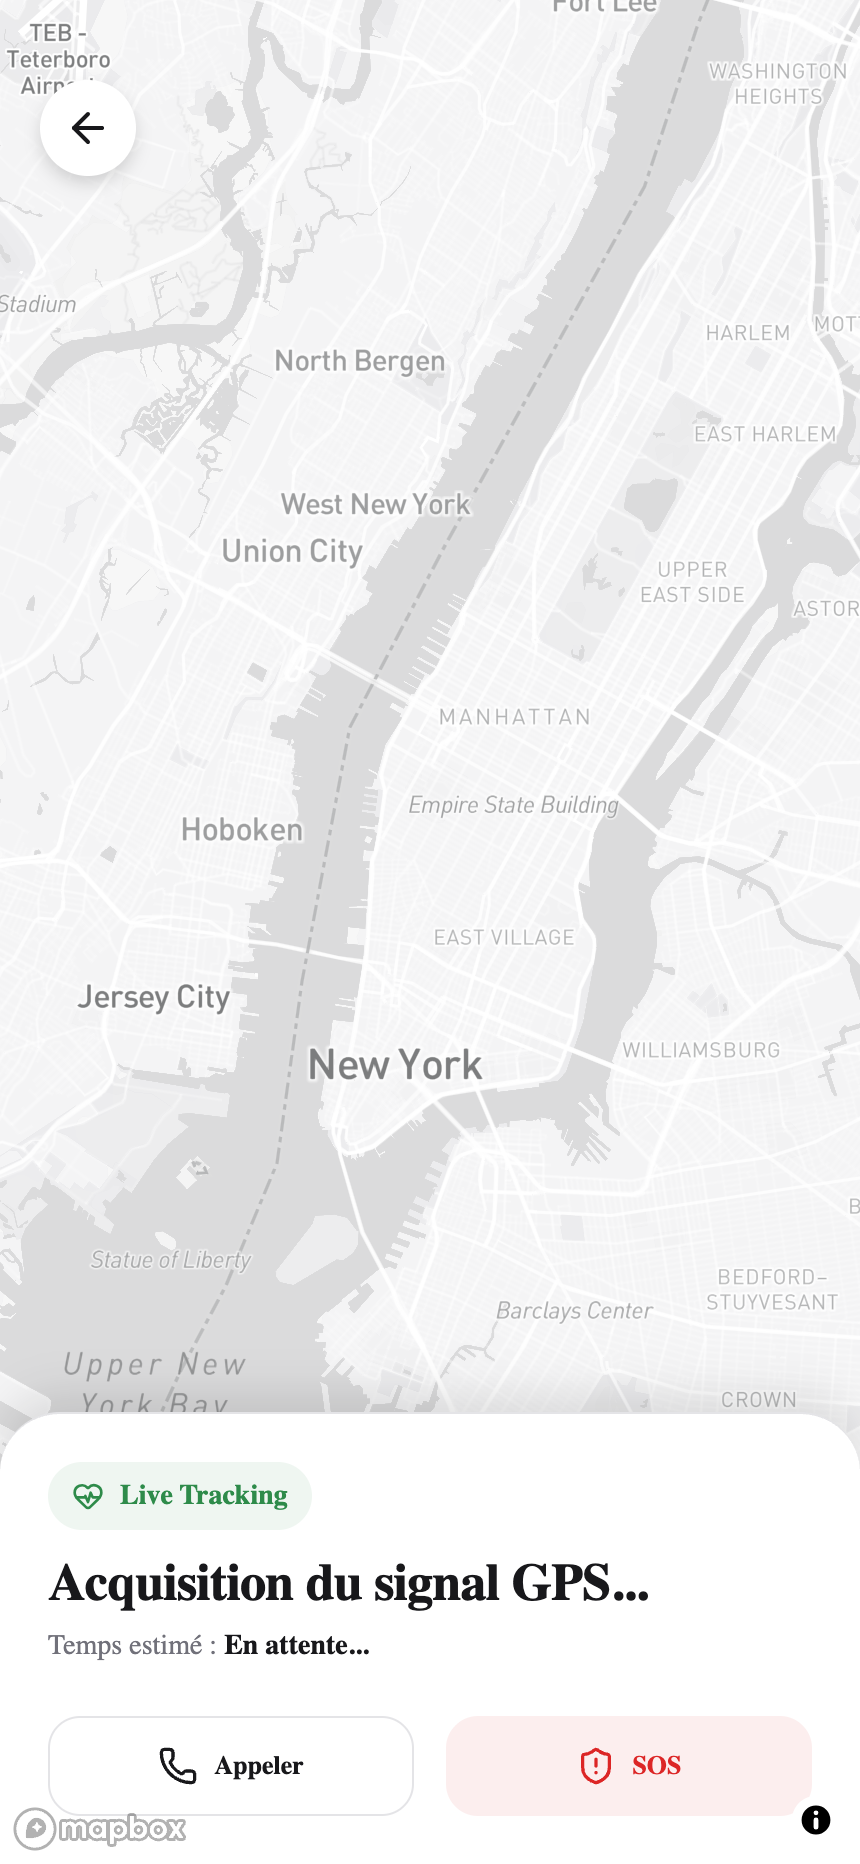
\includegraphics[width=\linewidth]{mobile-all/p_26_live_tracking.png}
    {\footnotesize D.26 --- Suivi GPS temps réel\par}
\end{minipage}\hfill
\begin{minipage}{0.30\textwidth}
    \centering
    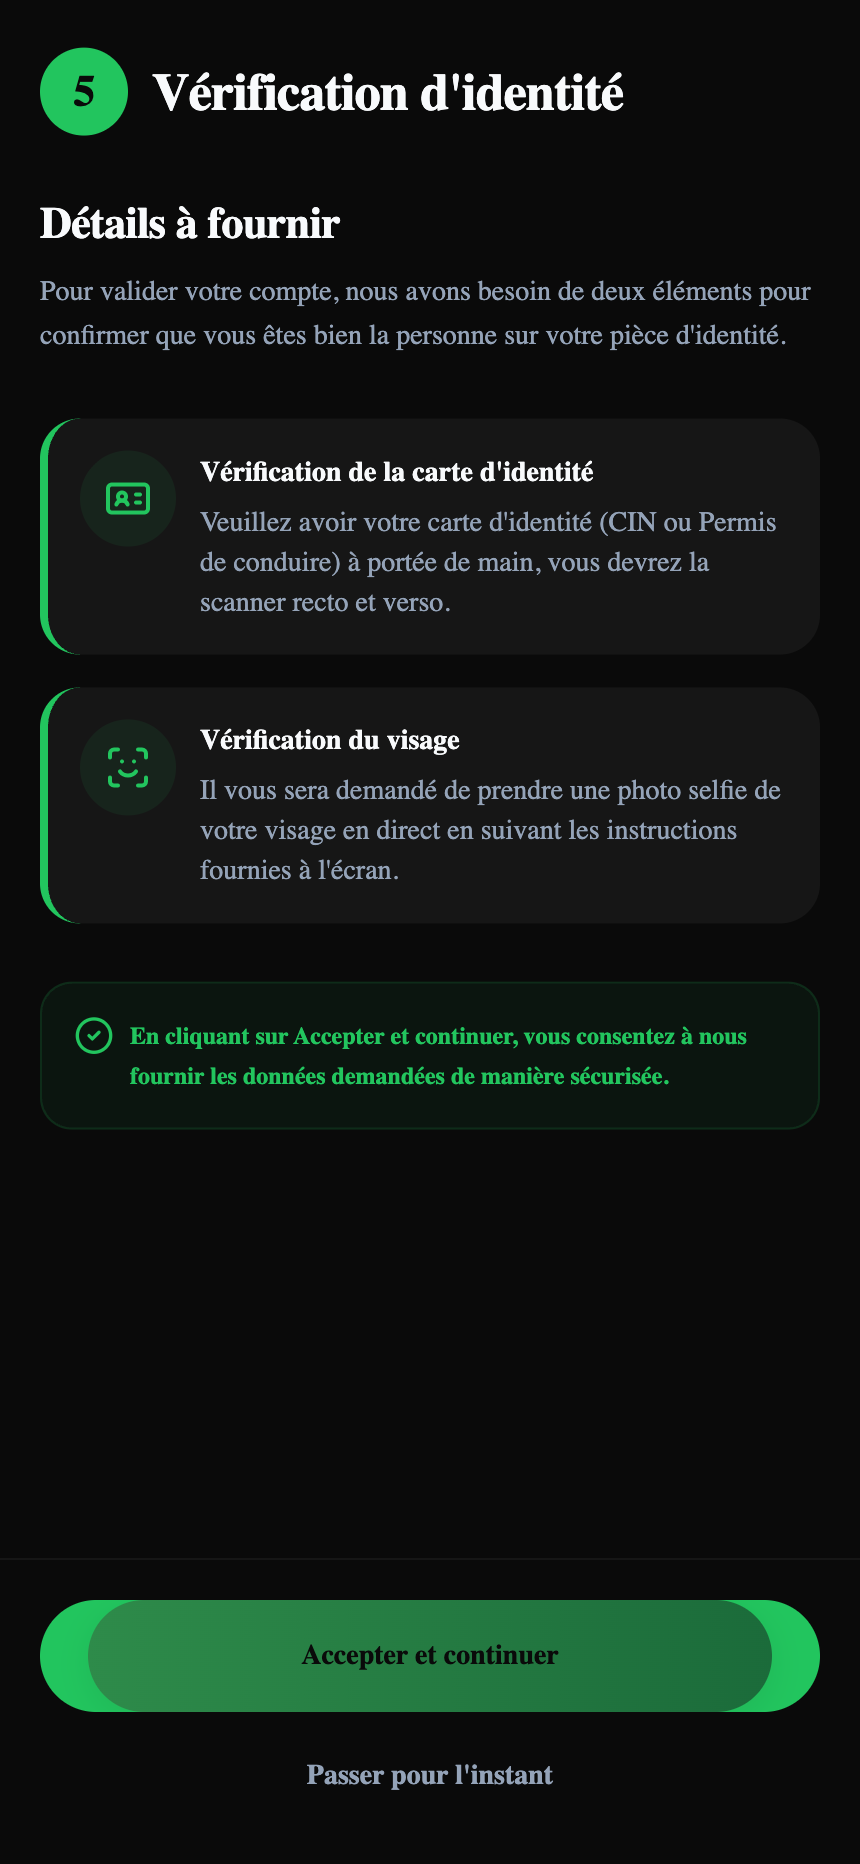
\includegraphics[width=\linewidth]{mobile-all/p_27_verif_intro.png}
    {\footnotesize D.27 --- Introduction KYC\par}
\end{minipage}
\end{figure}

\begin{figure}[H]
\centering
\begin{minipage}{0.30\textwidth}
    \centering
    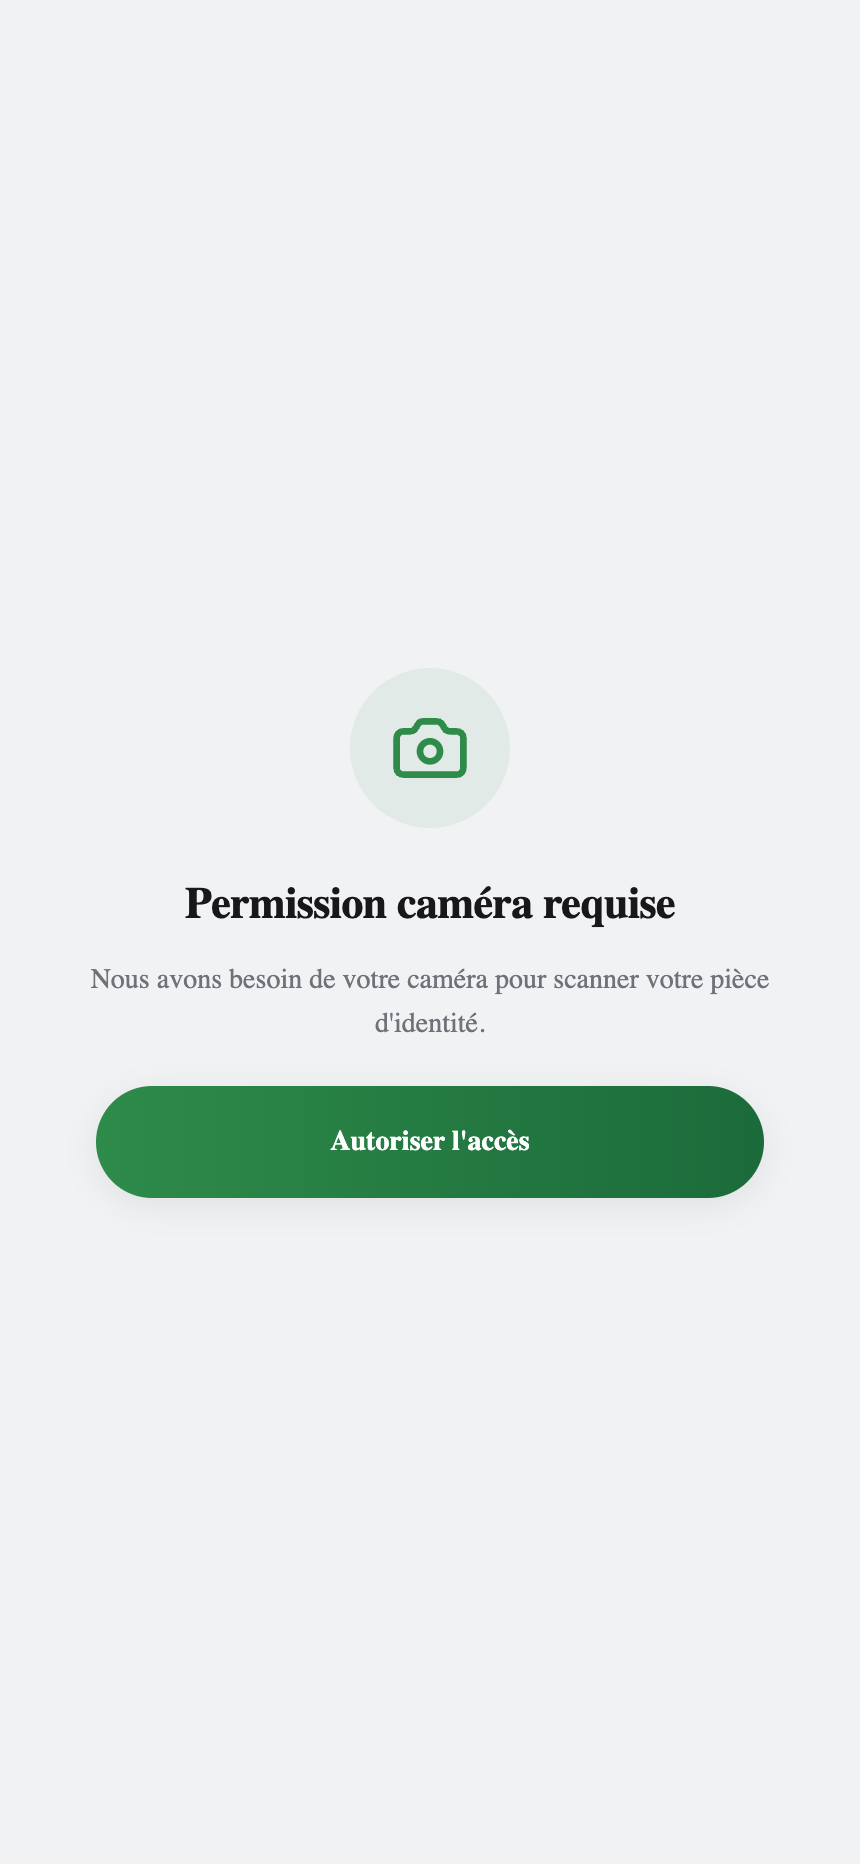
\includegraphics[width=\linewidth]{mobile-all/p_28_verif_id_capture.png}
    {\footnotesize D.28 --- Capture CIN\par}
\end{minipage}\hfill
\begin{minipage}{0.30\textwidth}
    \centering
    
\includegraphics[width=\linewidth]{mobile-all/p_29_verif_face_capture.png}
    {\footnotesize D.29 --- Capture vivacité\par}
\end{minipage}\hfill
\begin{minipage}{0.30\textwidth}
    \centering
    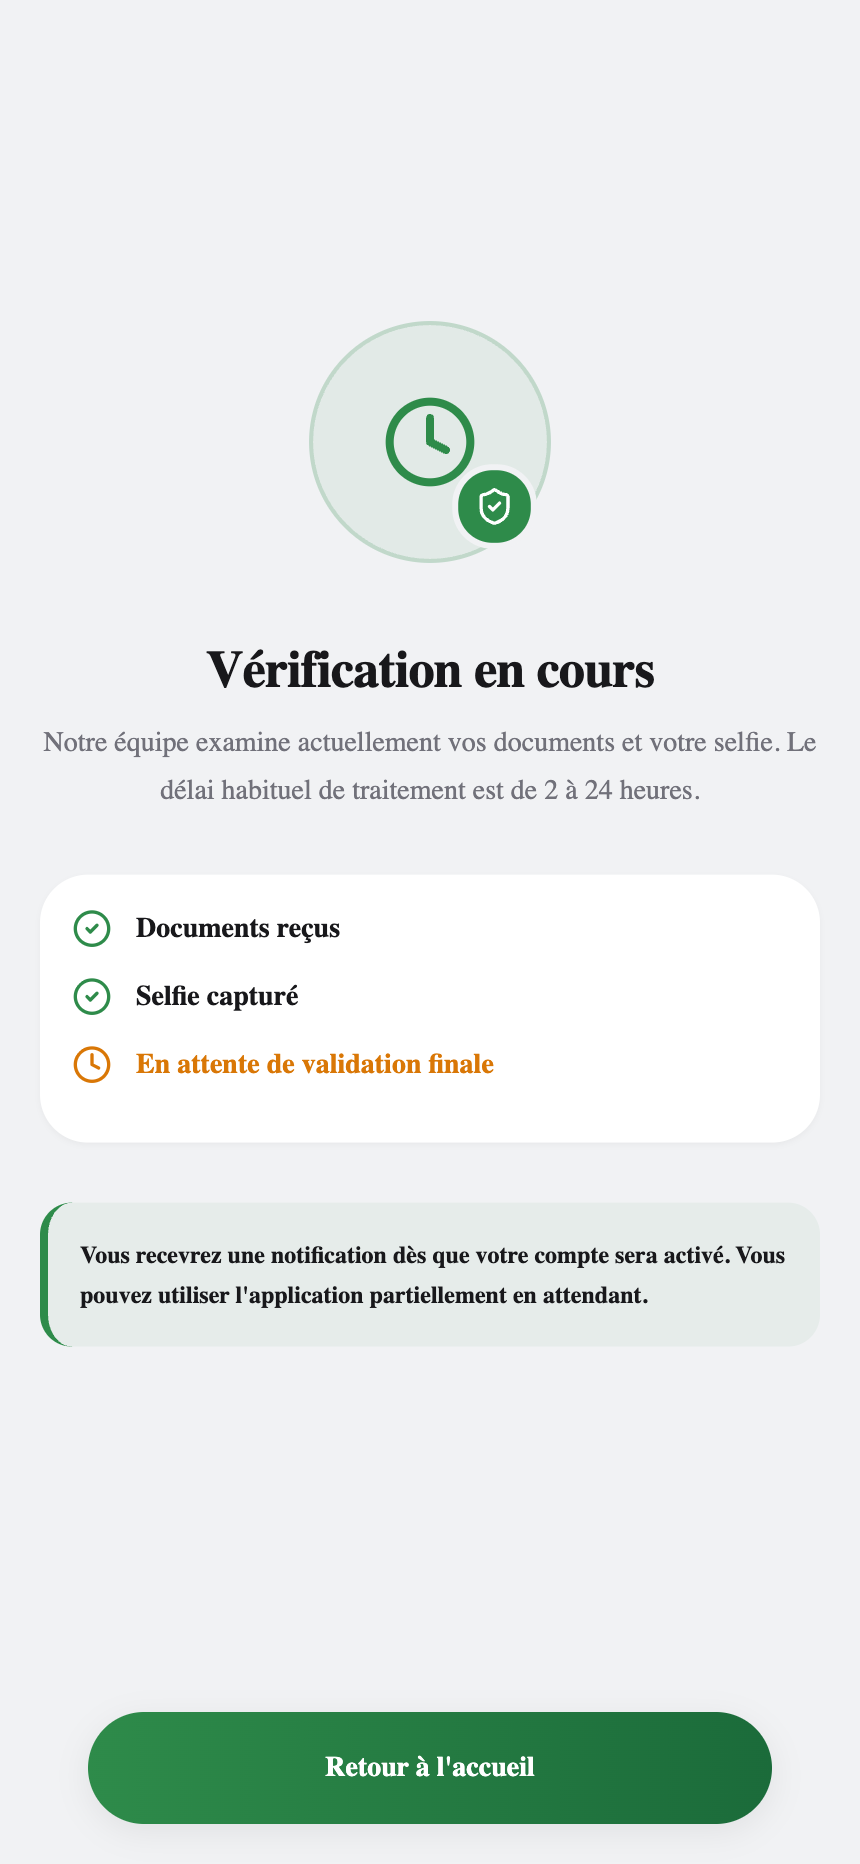
\includegraphics[width=\linewidth]{mobile-all/p_30_verif_pending.png}
    {\footnotesize D.30 --- KYC en attente\par}
\end{minipage}
\caption{Interfaces passager --- Écrans D.1 à D.30}
\end{figure}

\begin{figure}[H]
\centering
\begin{minipage}{0.30\textwidth}
    \centering
    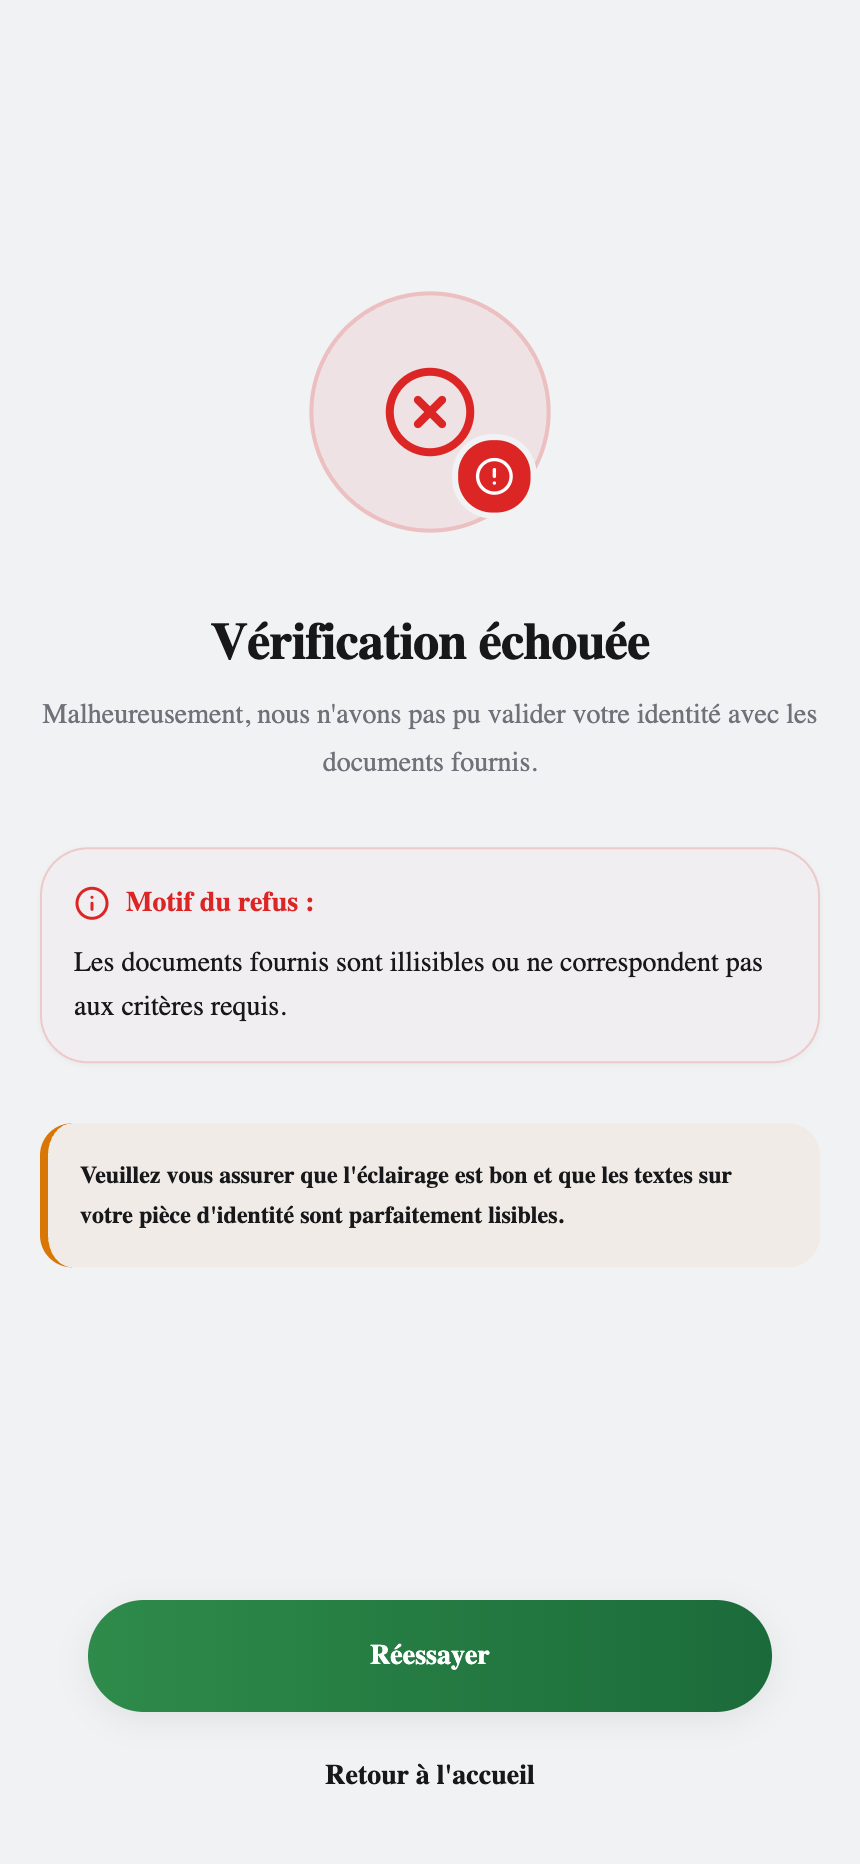
\includegraphics[width=\linewidth]{mobile-all/p_31_verif_rejected.png}
    {\footnotesize D.31 --- KYC rejeté (passager)\par}
\end{minipage}
\caption{Interface passager --- Écran D.31}
\end{figure}

% ----------------------------------------------------------------
\section{Parcours conducteur --- 31 écrans}
% ----------------------------------------------------------------

\begin{figure}[H]
\centering
\begin{minipage}{0.30\textwidth}
    \centering
    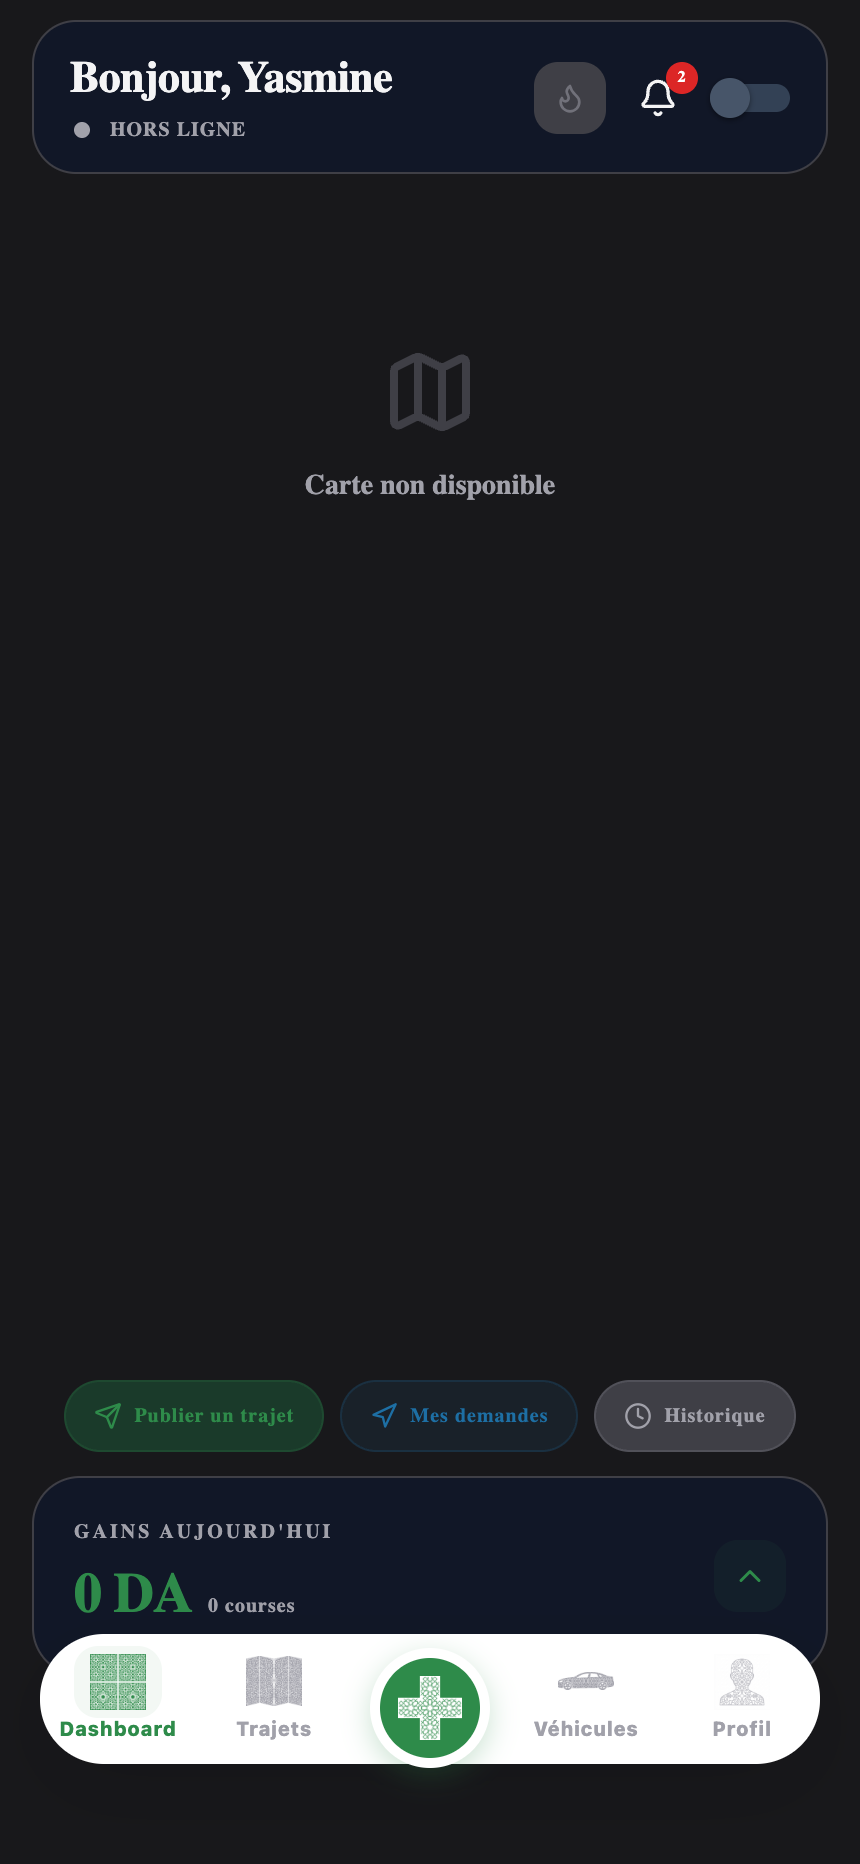
\includegraphics[width=\linewidth]{mobile-all/d_01_tab_dashboard.png}
    {\footnotesize D.32 --- Dashboard conducteur\par}
\end{minipage}\hfill
\begin{minipage}{0.30\textwidth}
    \centering
    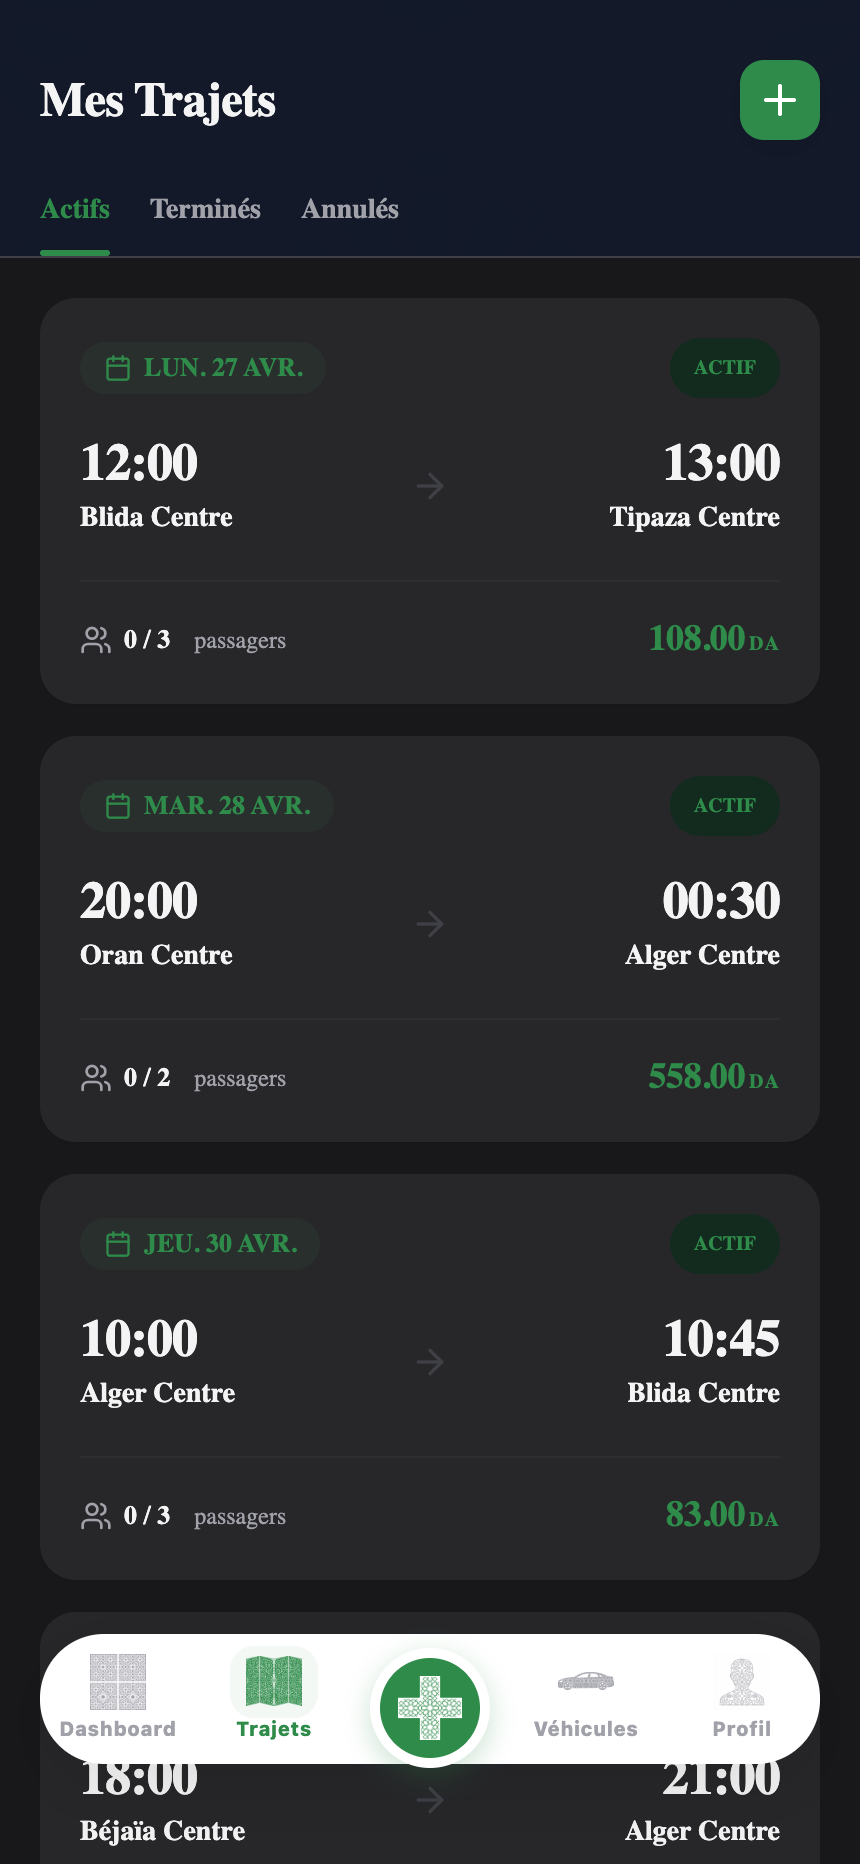
\includegraphics[width=\linewidth]{mobile-all/d_02_tab_trips.png}
    {\footnotesize D.33 --- Mes trajets (conducteur)\par}
\end{minipage}\hfill
\begin{minipage}{0.30\textwidth}
    \centering
    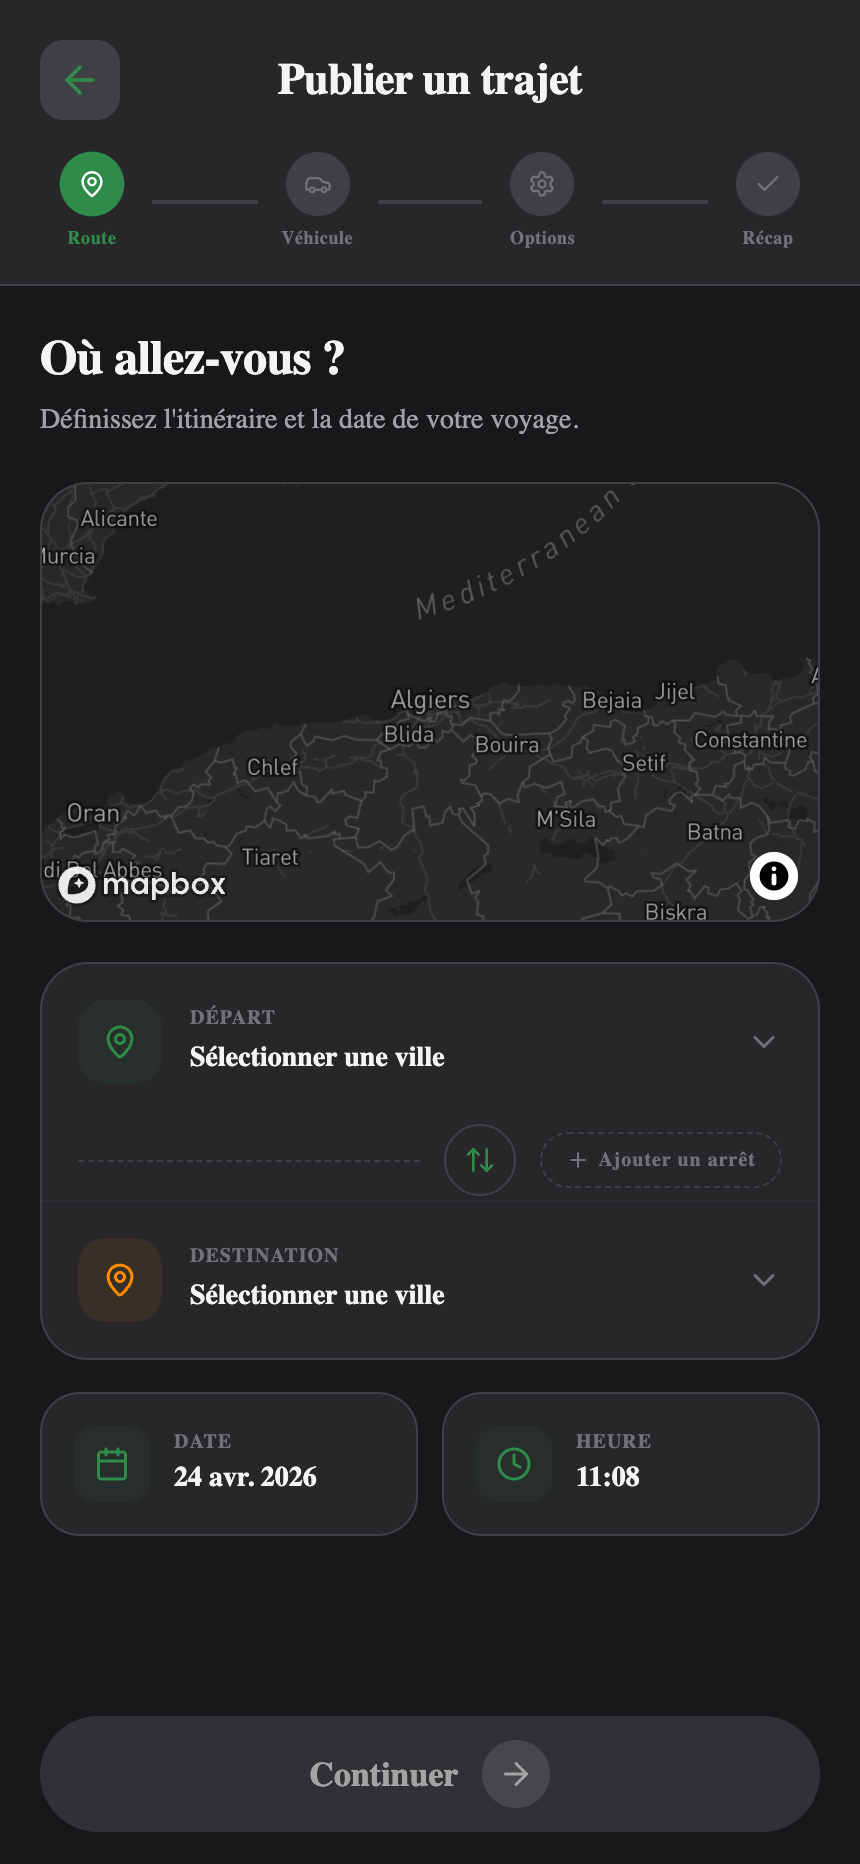
\includegraphics[width=\linewidth]{mobile-all/d_03_tab_publish.png}
    {\footnotesize D.34 --- Publication trajet\par}
\end{minipage}
\end{figure}

\begin{figure}[H]
\centering
\begin{minipage}{0.30\textwidth}
    \centering
    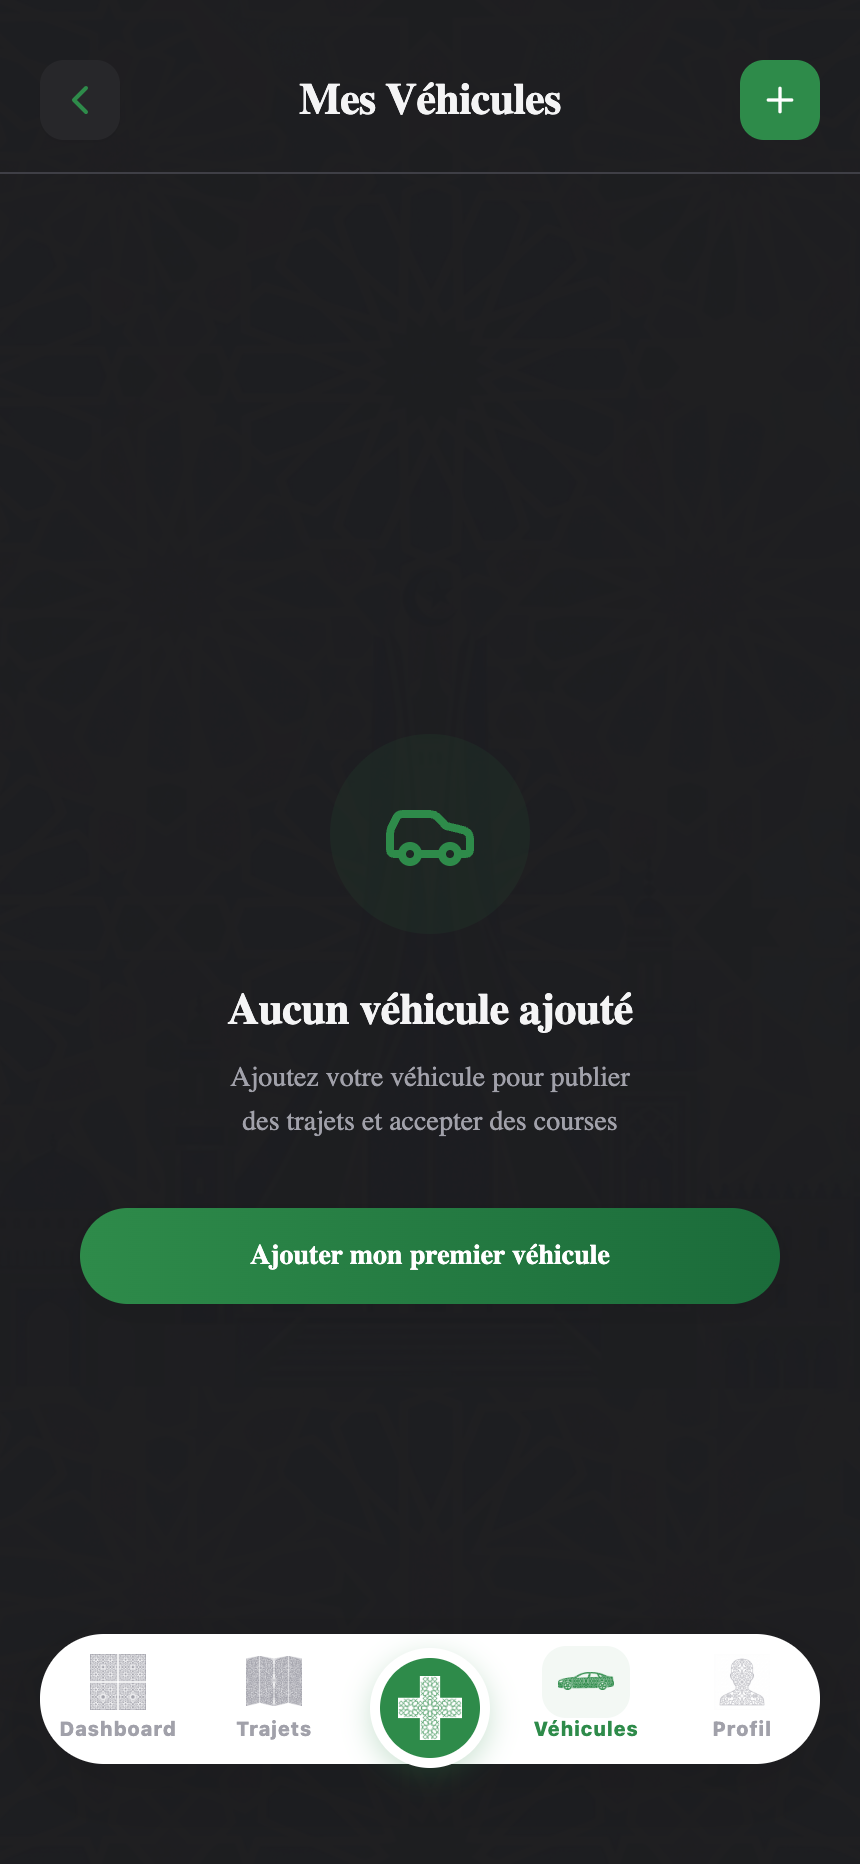
\includegraphics[width=\linewidth]{mobile-all/d_04_tab_vehicles.png}
    {\footnotesize D.35 --- Onglet véhicules\par}
\end{minipage}\hfill
\begin{minipage}{0.30\textwidth}
    \centering
    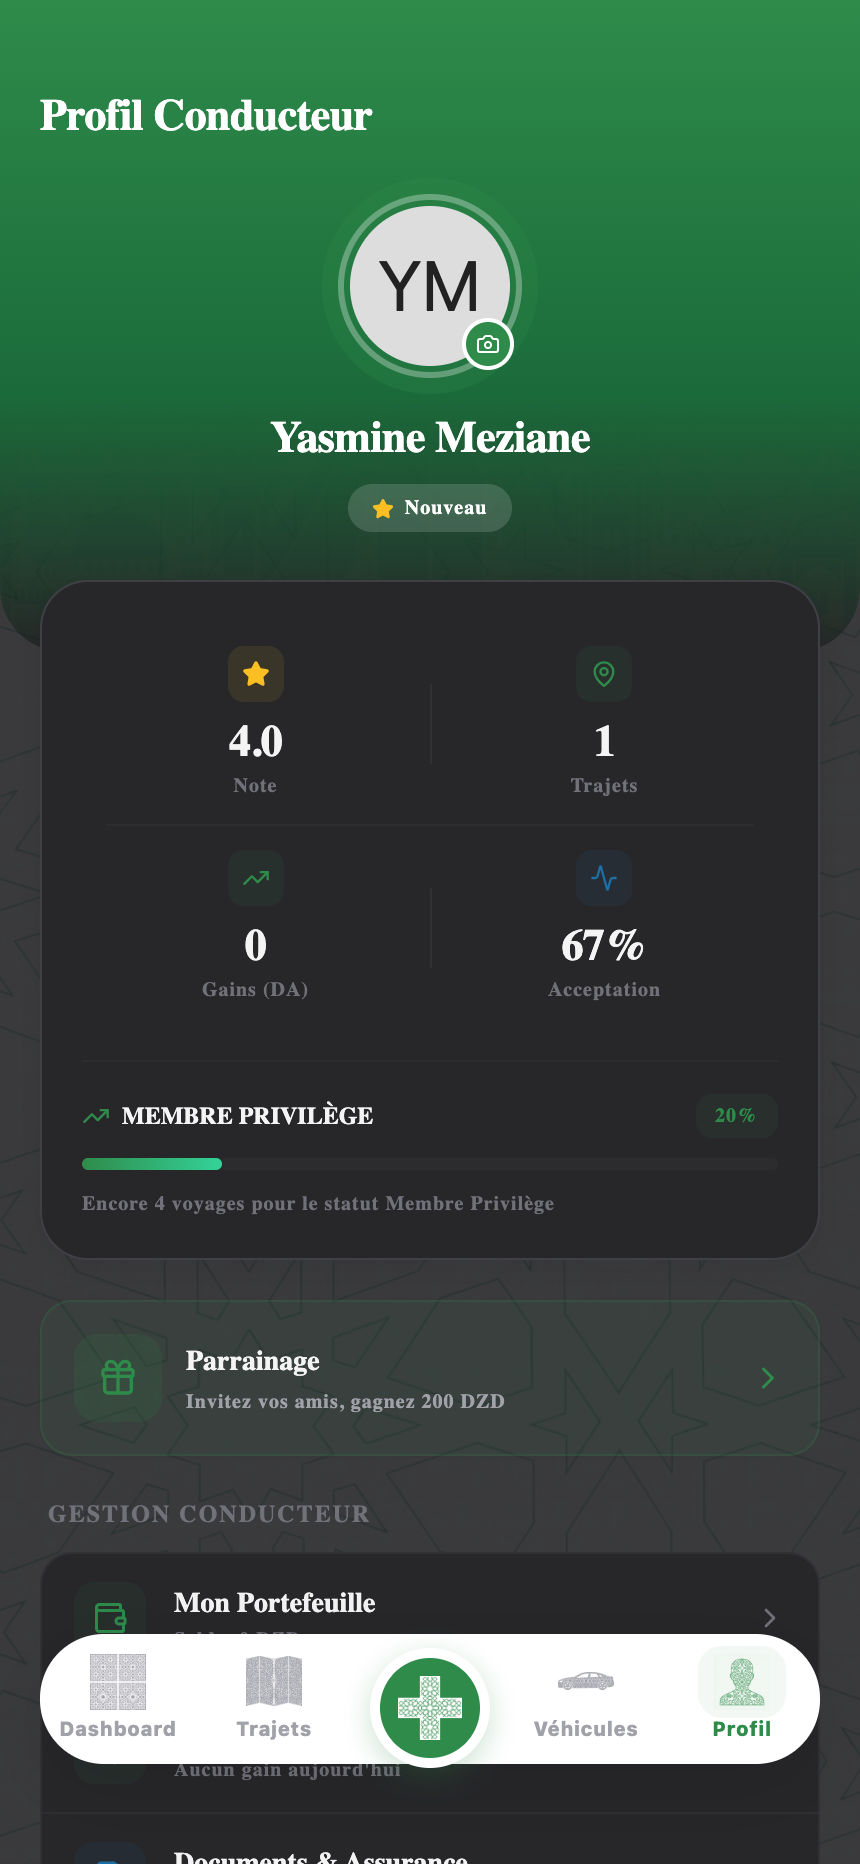
\includegraphics[width=\linewidth]{mobile-all/d_05_tab_profile.png}
    {\footnotesize D.36 --- Profil conducteur\par}
\end{minipage}\hfill
\begin{minipage}{0.30\textwidth}
    \centering
    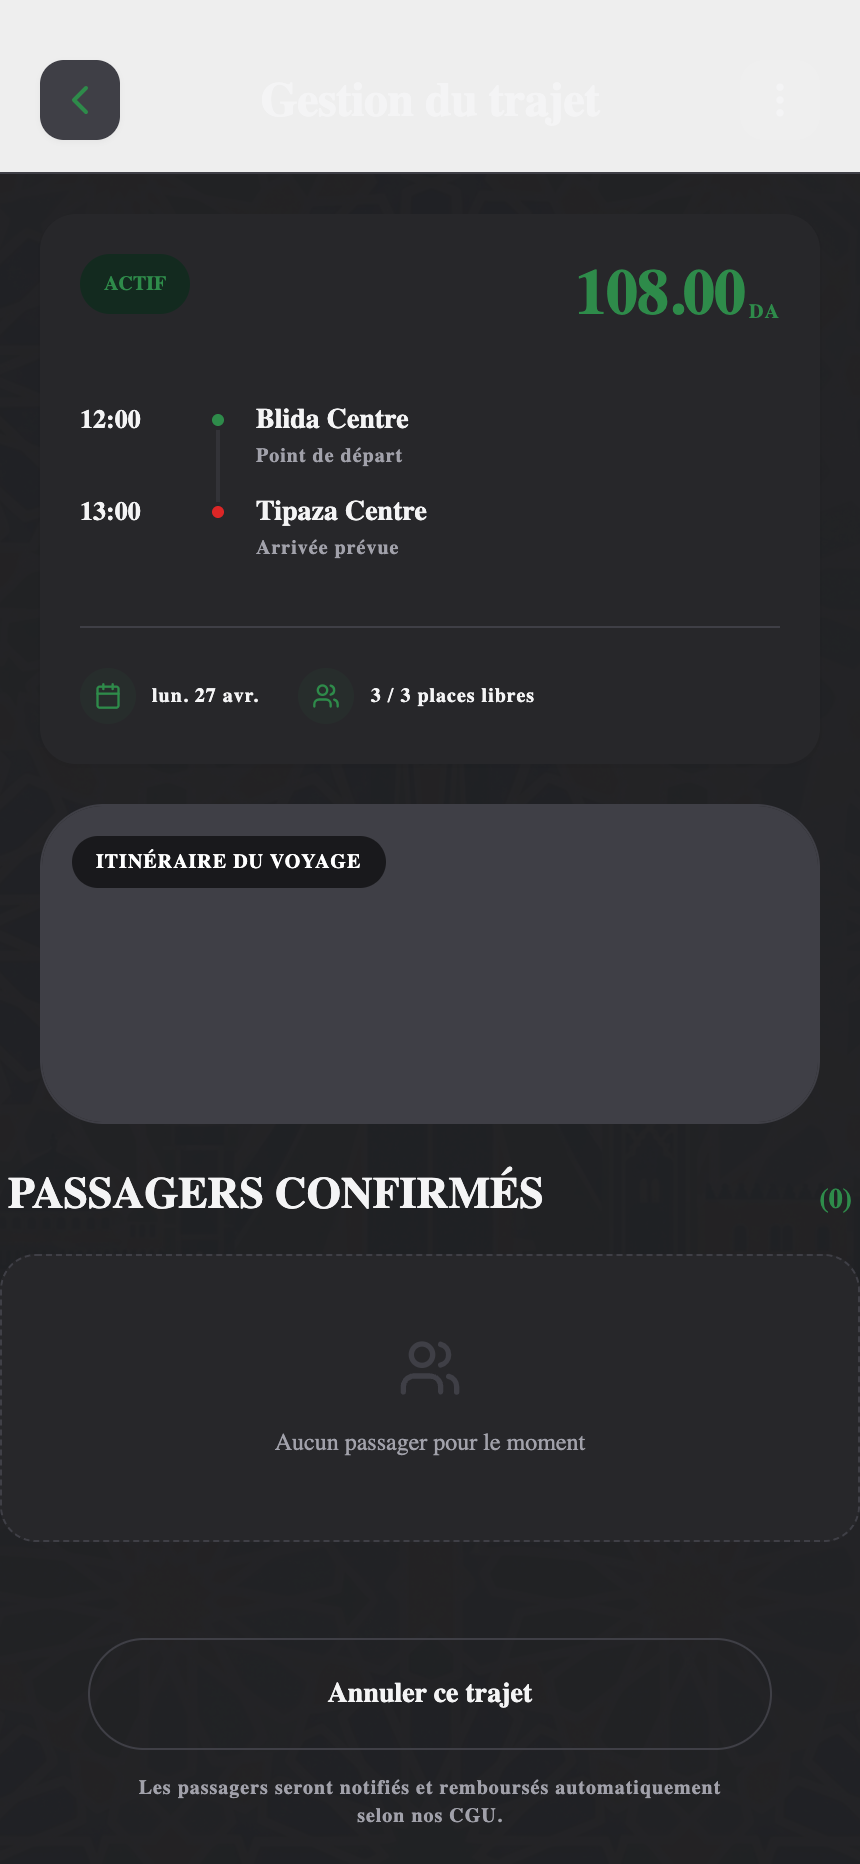
\includegraphics[width=\linewidth]{mobile-all/d_06_trip_manage.png}
    {\footnotesize D.37 --- Gestion du trajet\par}
\end{minipage}
\end{figure}

\begin{figure}[H]
\centering
\begin{minipage}{0.30\textwidth}
    \centering
    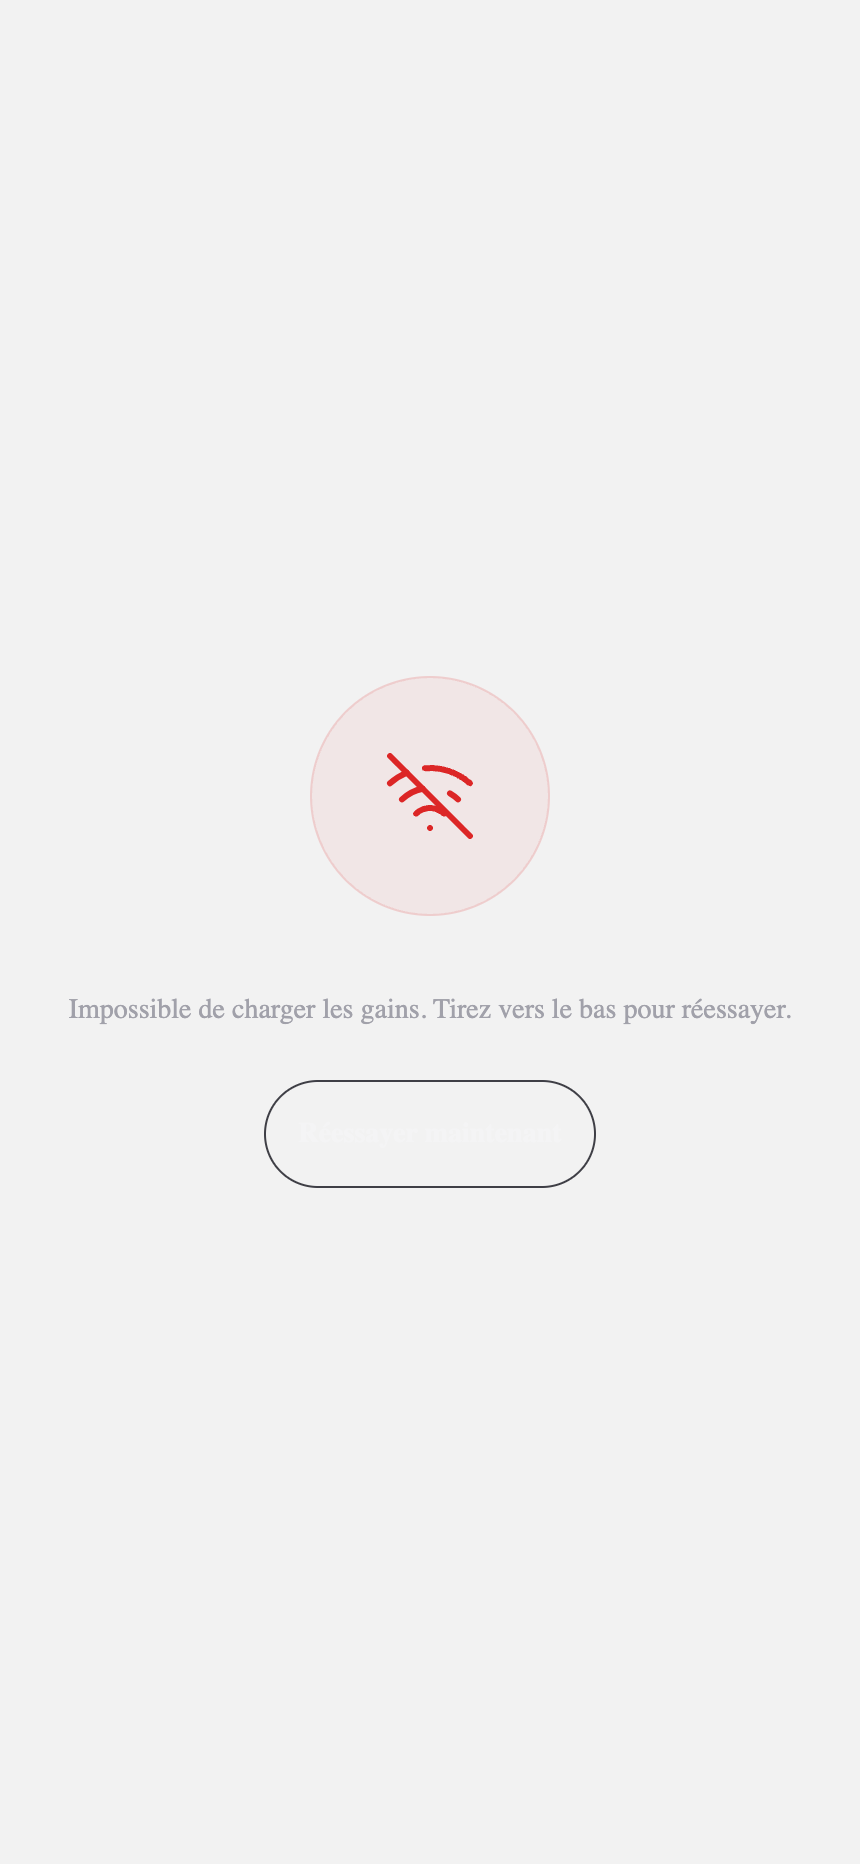
\includegraphics[width=\linewidth]{mobile-all/d_07_earnings.png}
    {\footnotesize D.38 --- Gains mensuels\par}
\end{minipage}\hfill
\begin{minipage}{0.30\textwidth}
    \centering
    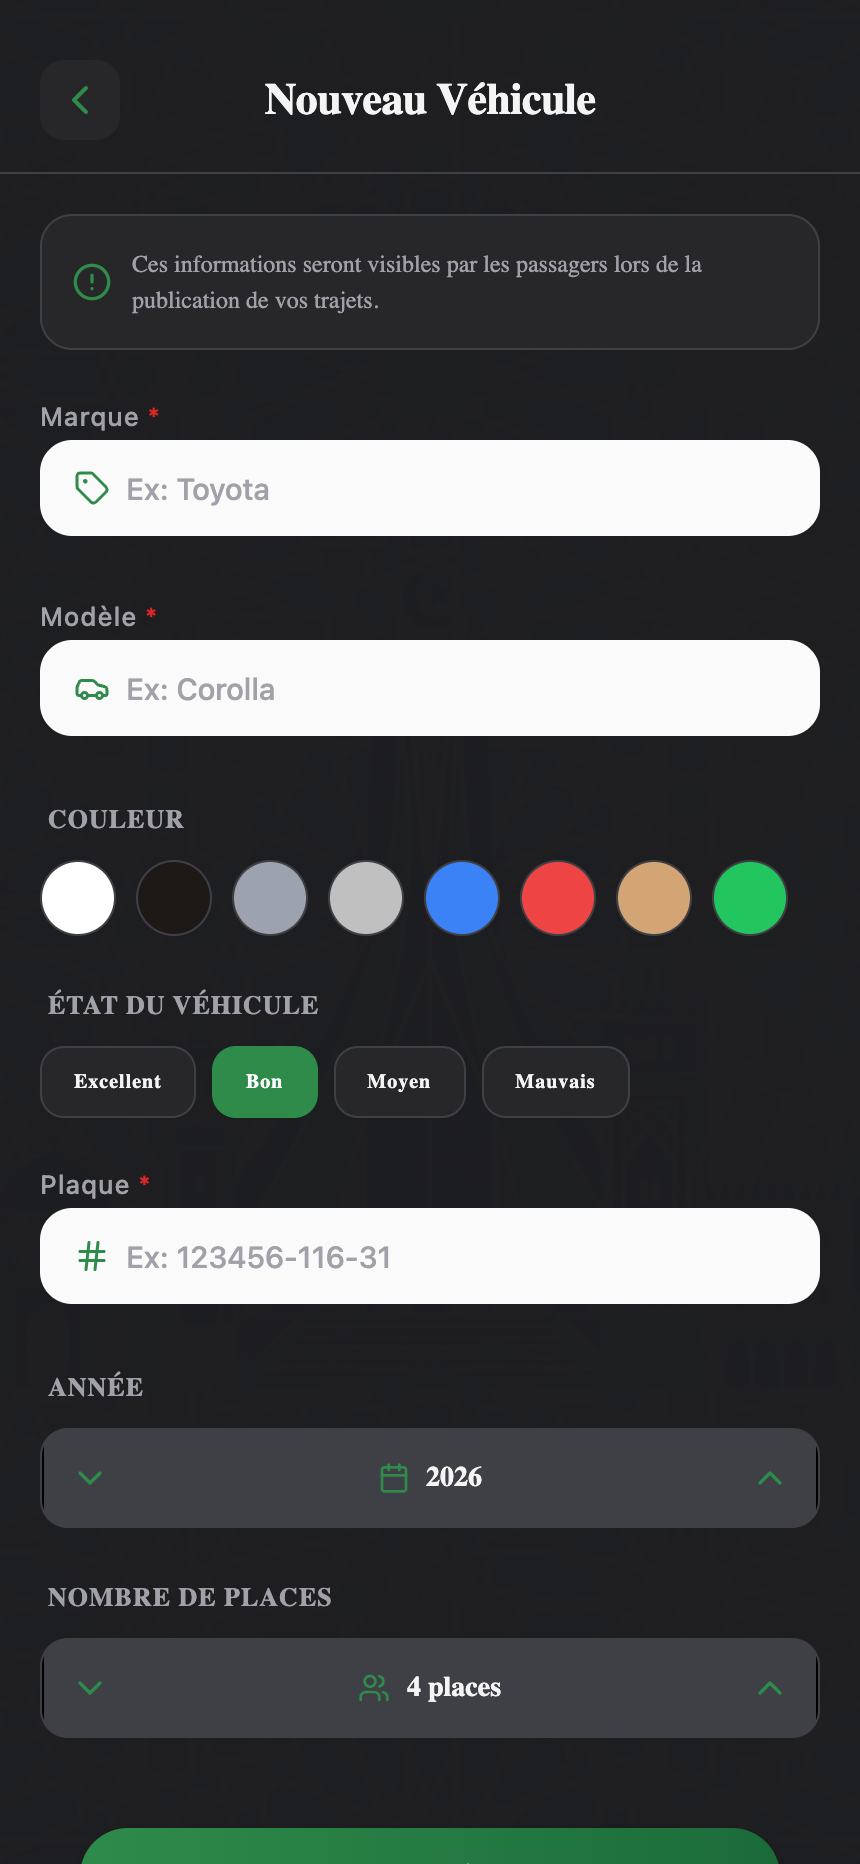
\includegraphics[width=\linewidth]{mobile-all/d_08_add_vehicle.png}
    {\footnotesize D.39 --- Ajout véhicule\par}
\end{minipage}\hfill
\begin{minipage}{0.30\textwidth}
    \centering
    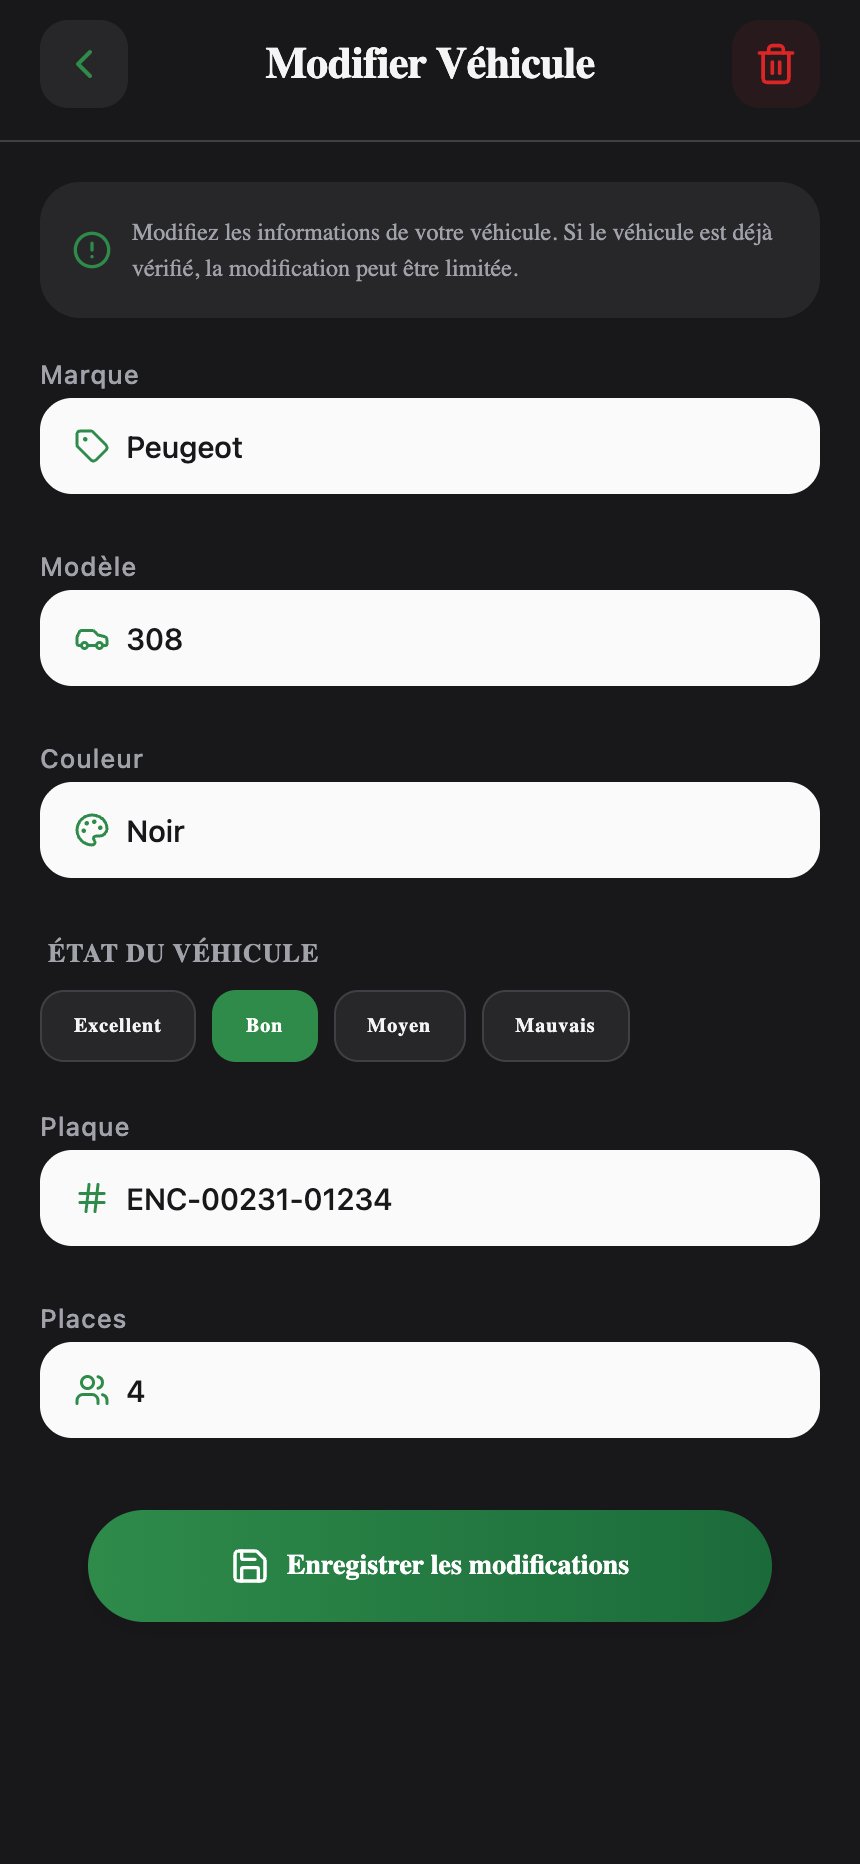
\includegraphics[width=\linewidth]{mobile-all/d_09_edit_vehicle.png}
    {\footnotesize D.40 --- Modifier véhicule\par}
\end{minipage}
\end{figure}

\begin{figure}[H]
\centering
\begin{minipage}{0.30\textwidth}
    \centering
    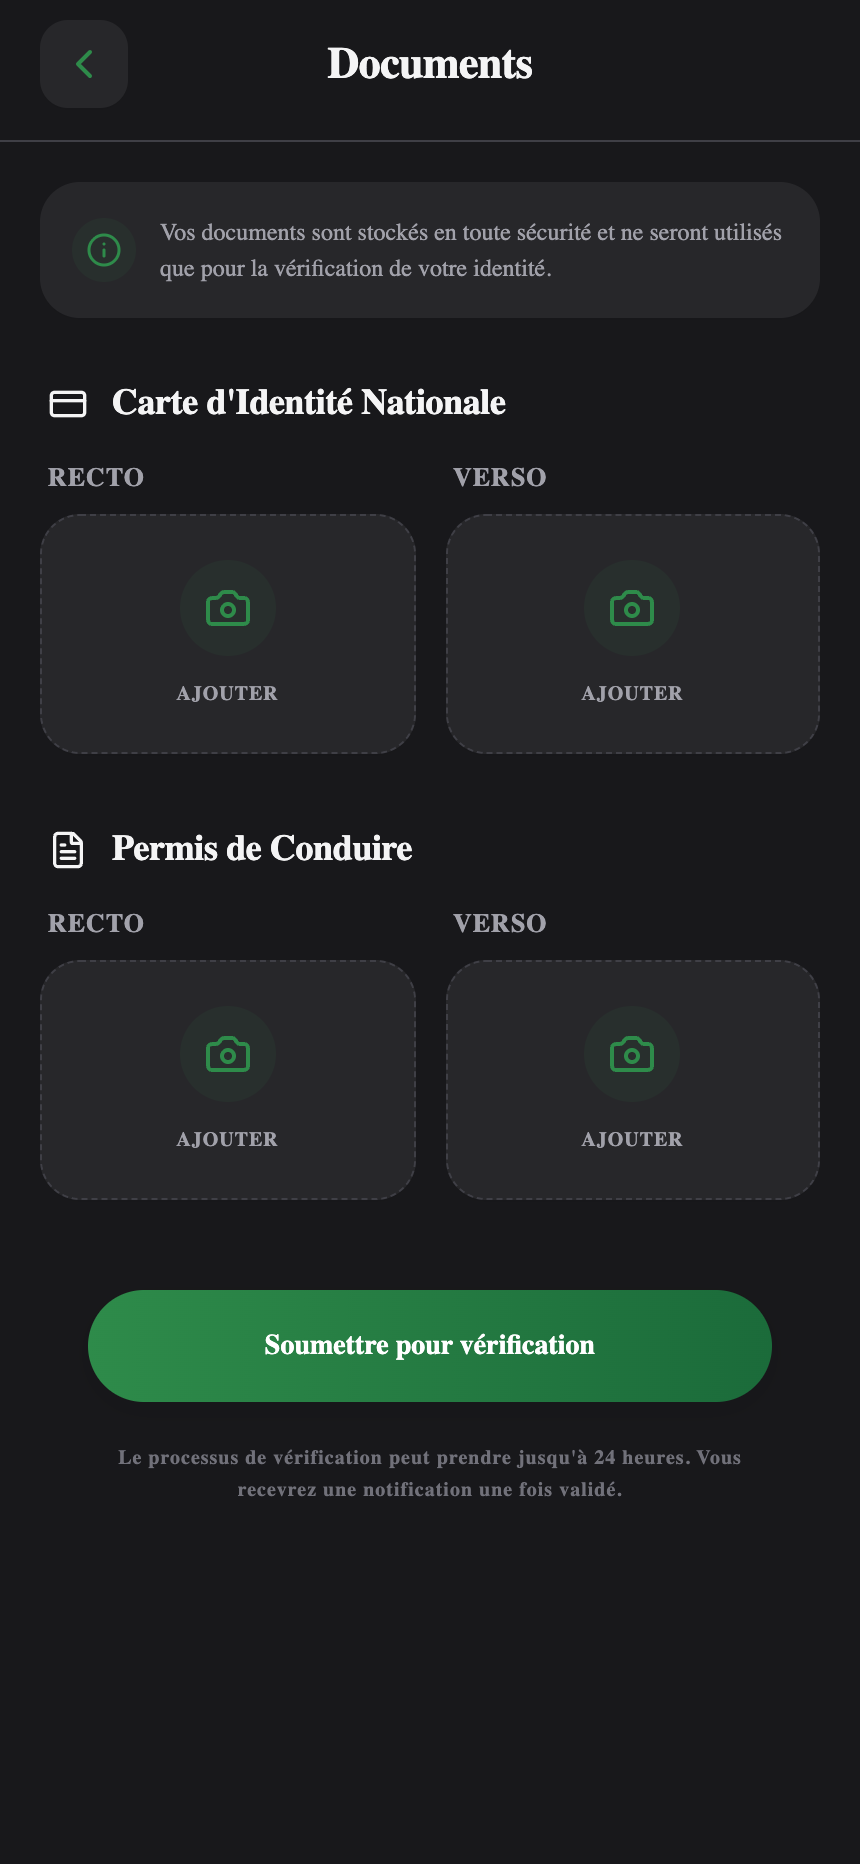
\includegraphics[width=\linewidth]{mobile-all/d_10_documents.png}
    {\footnotesize D.41 --- Documents véhicule\par}
\end{minipage}\hfill
\begin{minipage}{0.30\textwidth}
    \centering
    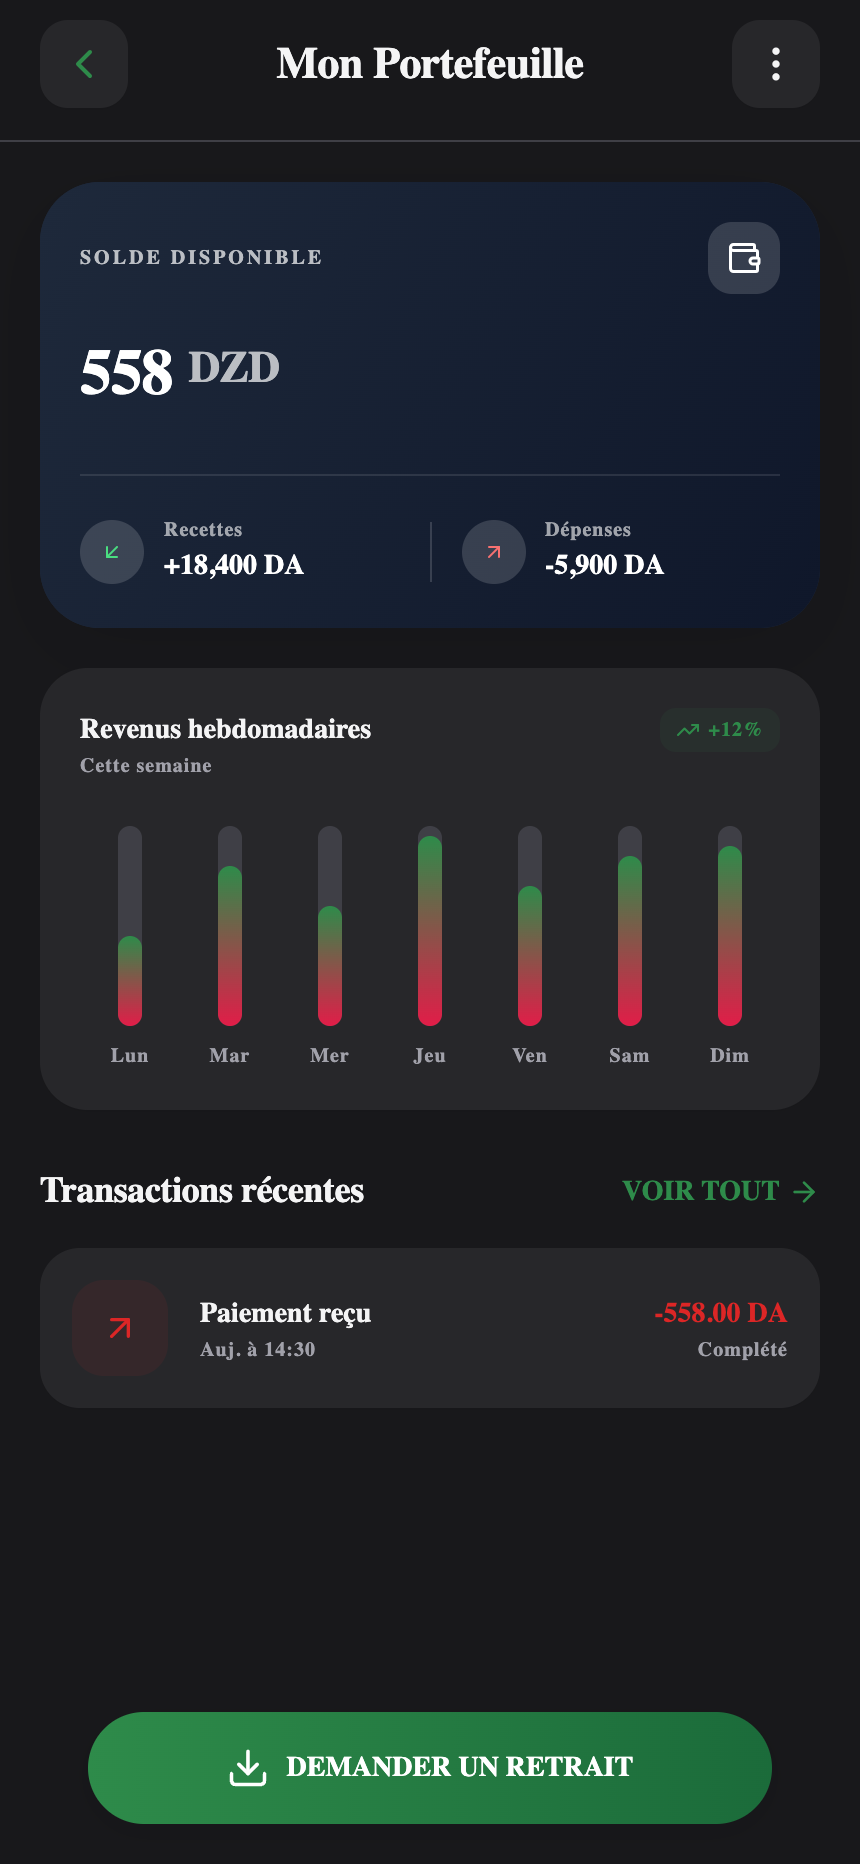
\includegraphics[width=\linewidth]{mobile-all/d_11_wallet.png}
    {\footnotesize D.42 --- Portefeuille\par}
\end{minipage}\hfill
\begin{minipage}{0.30\textwidth}
    \centering
    
\includegraphics[width=\linewidth]{mobile-all/d_12_trip_requests.png}
    {\footnotesize D.43 --- Demandes de trajet\par}
\end{minipage}
\end{figure}

\begin{figure}[H]
\centering
\begin{minipage}{0.30\textwidth}
    \centering
    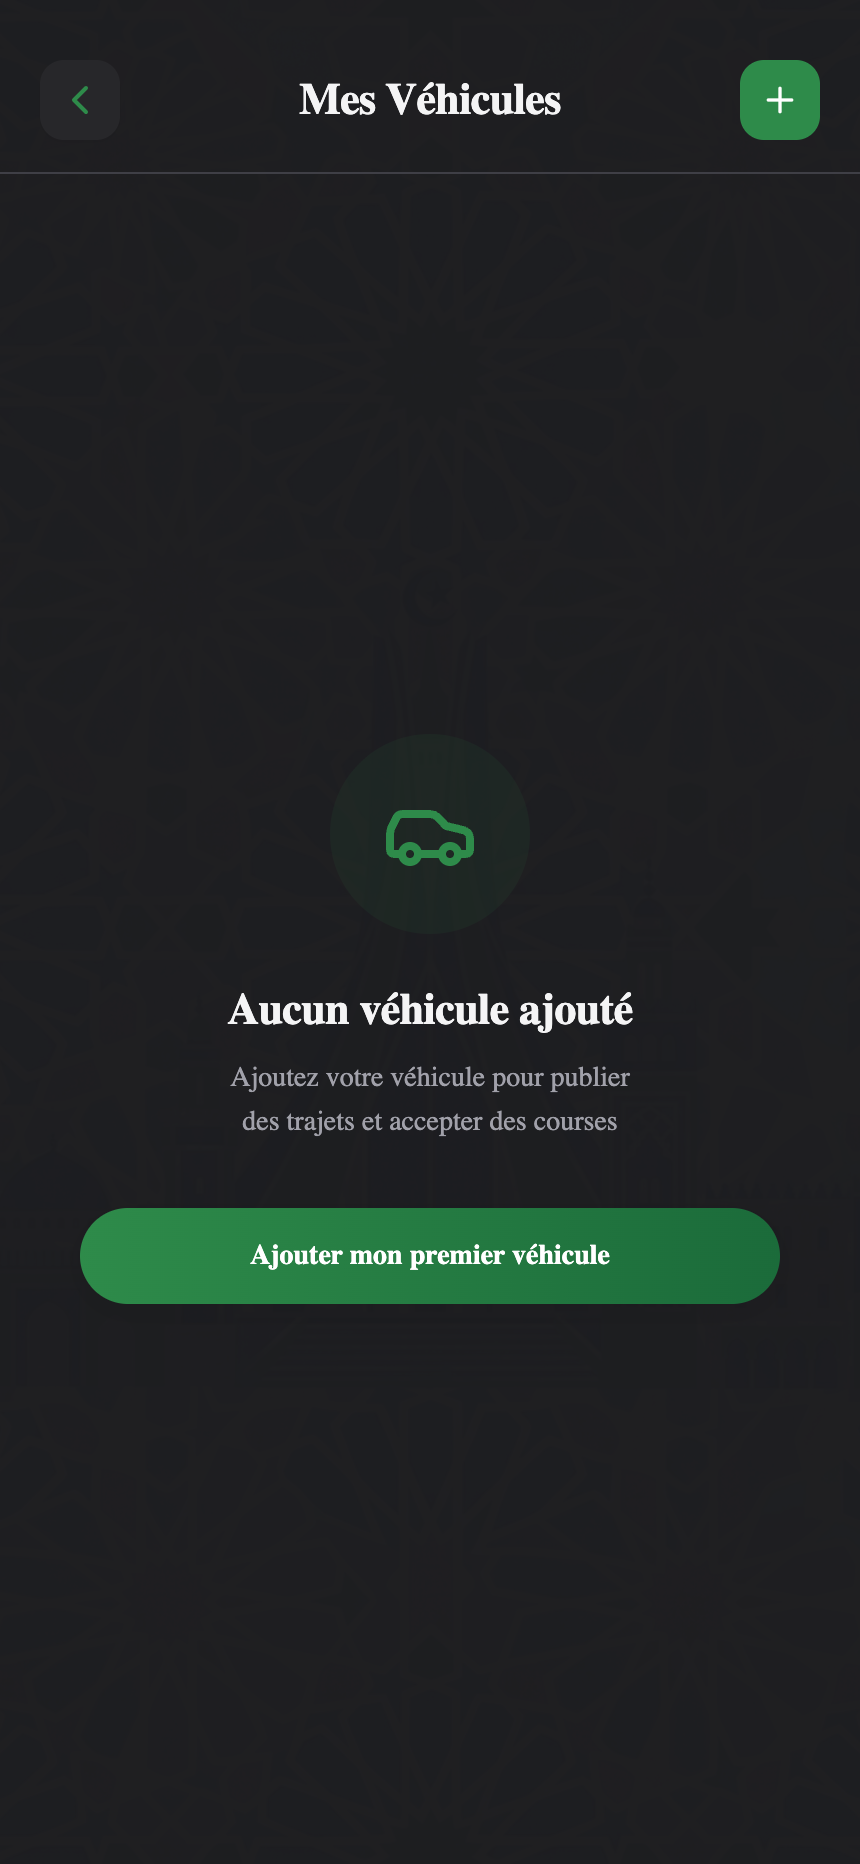
\includegraphics[width=\linewidth]{mobile-all/d_13_vehicles_list.png}
    {\footnotesize D.44 --- Liste véhicules\par}
\end{minipage}\hfill
\begin{minipage}{0.30\textwidth}
    \centering
    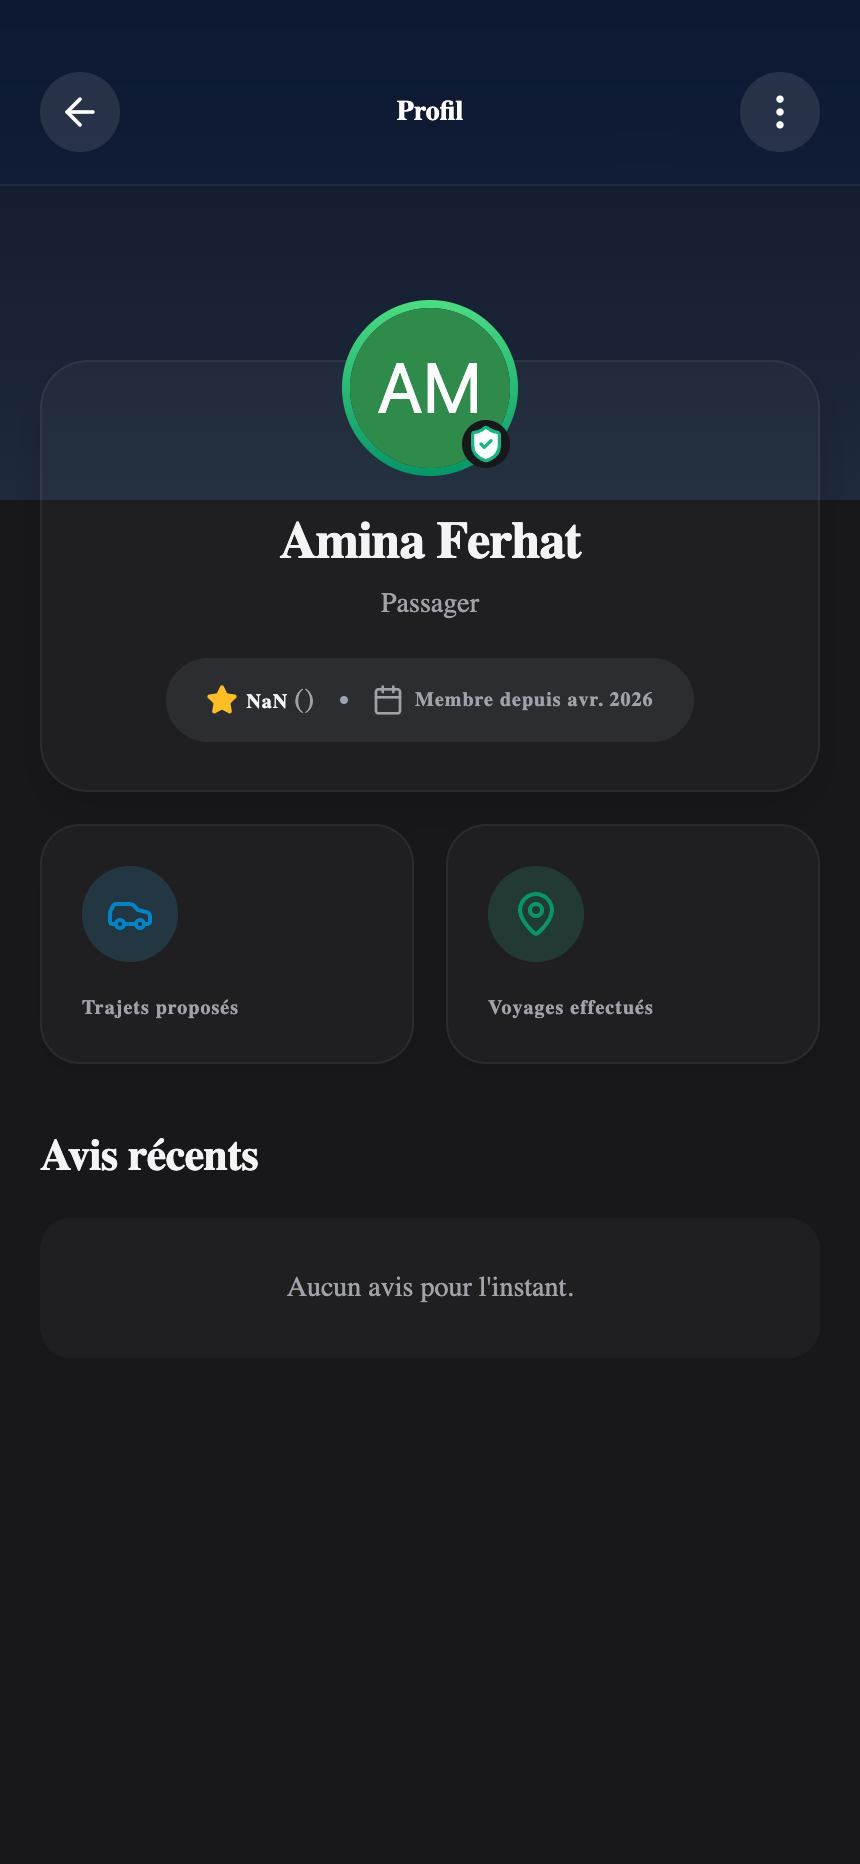
\includegraphics[width=\linewidth]{mobile-all/d_14_public_profile.png}
    {\footnotesize D.45 --- Profil public\par}
\end{minipage}\hfill
\begin{minipage}{0.30\textwidth}
    \centering
    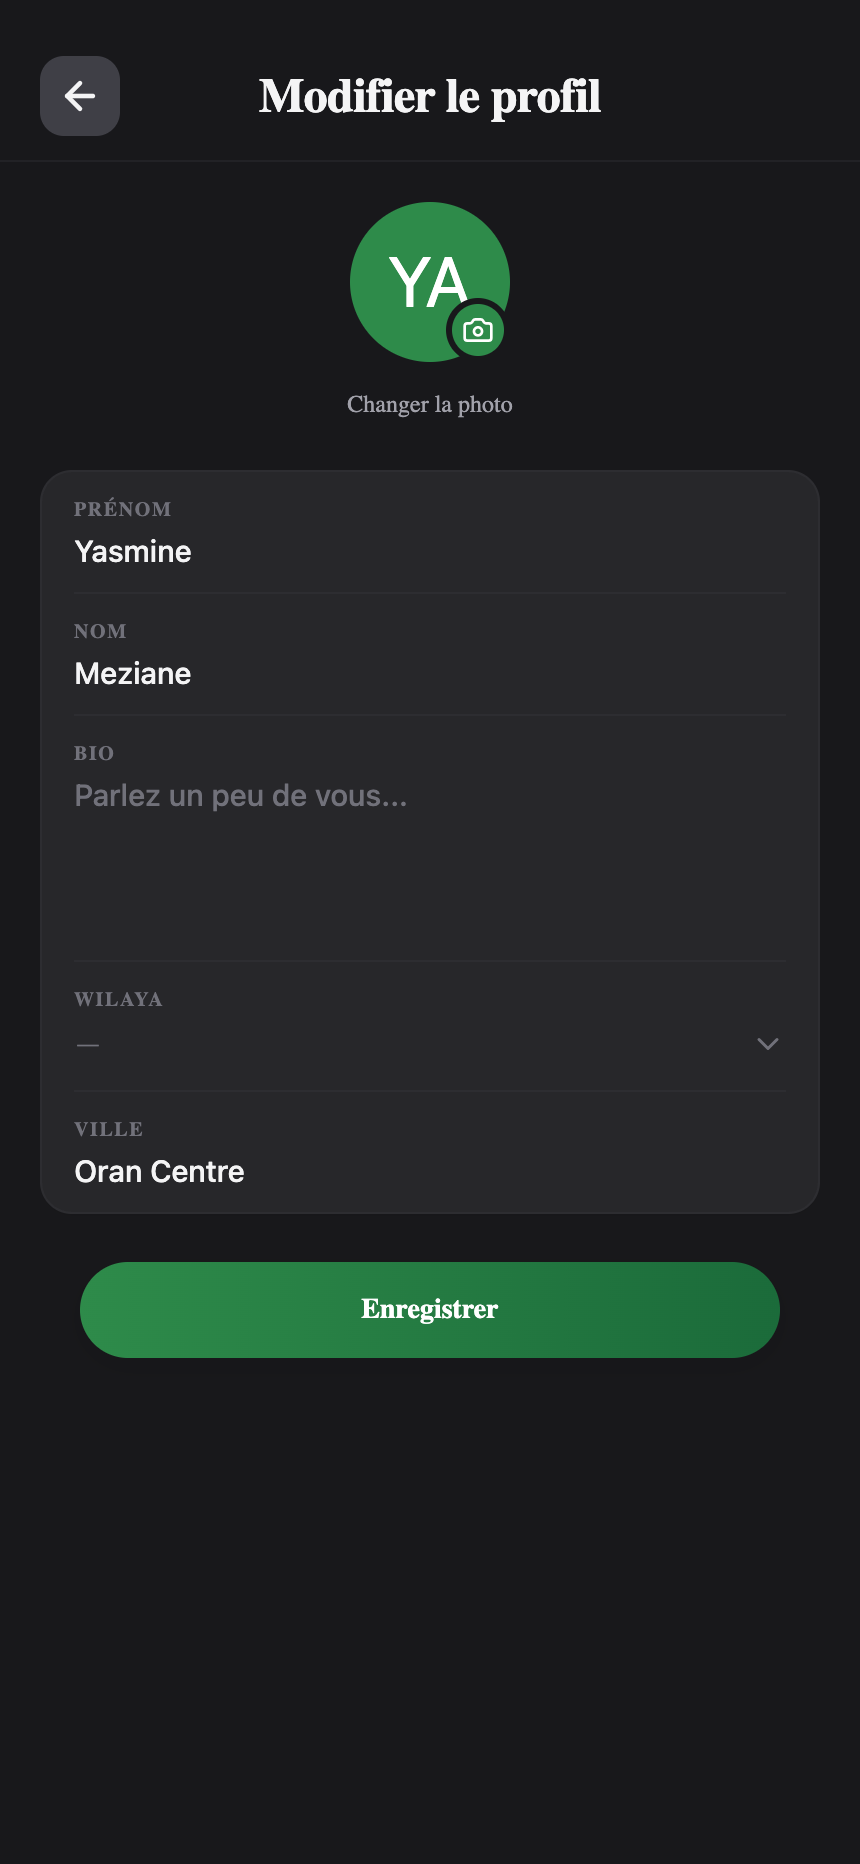
\includegraphics[width=\linewidth]{mobile-all/d_15_edit_profile.png}
    {\footnotesize D.46 --- Modifier profil\par}
\end{minipage}
\end{figure}

\begin{figure}[H]
\centering
\begin{minipage}{0.30\textwidth}
    \centering
    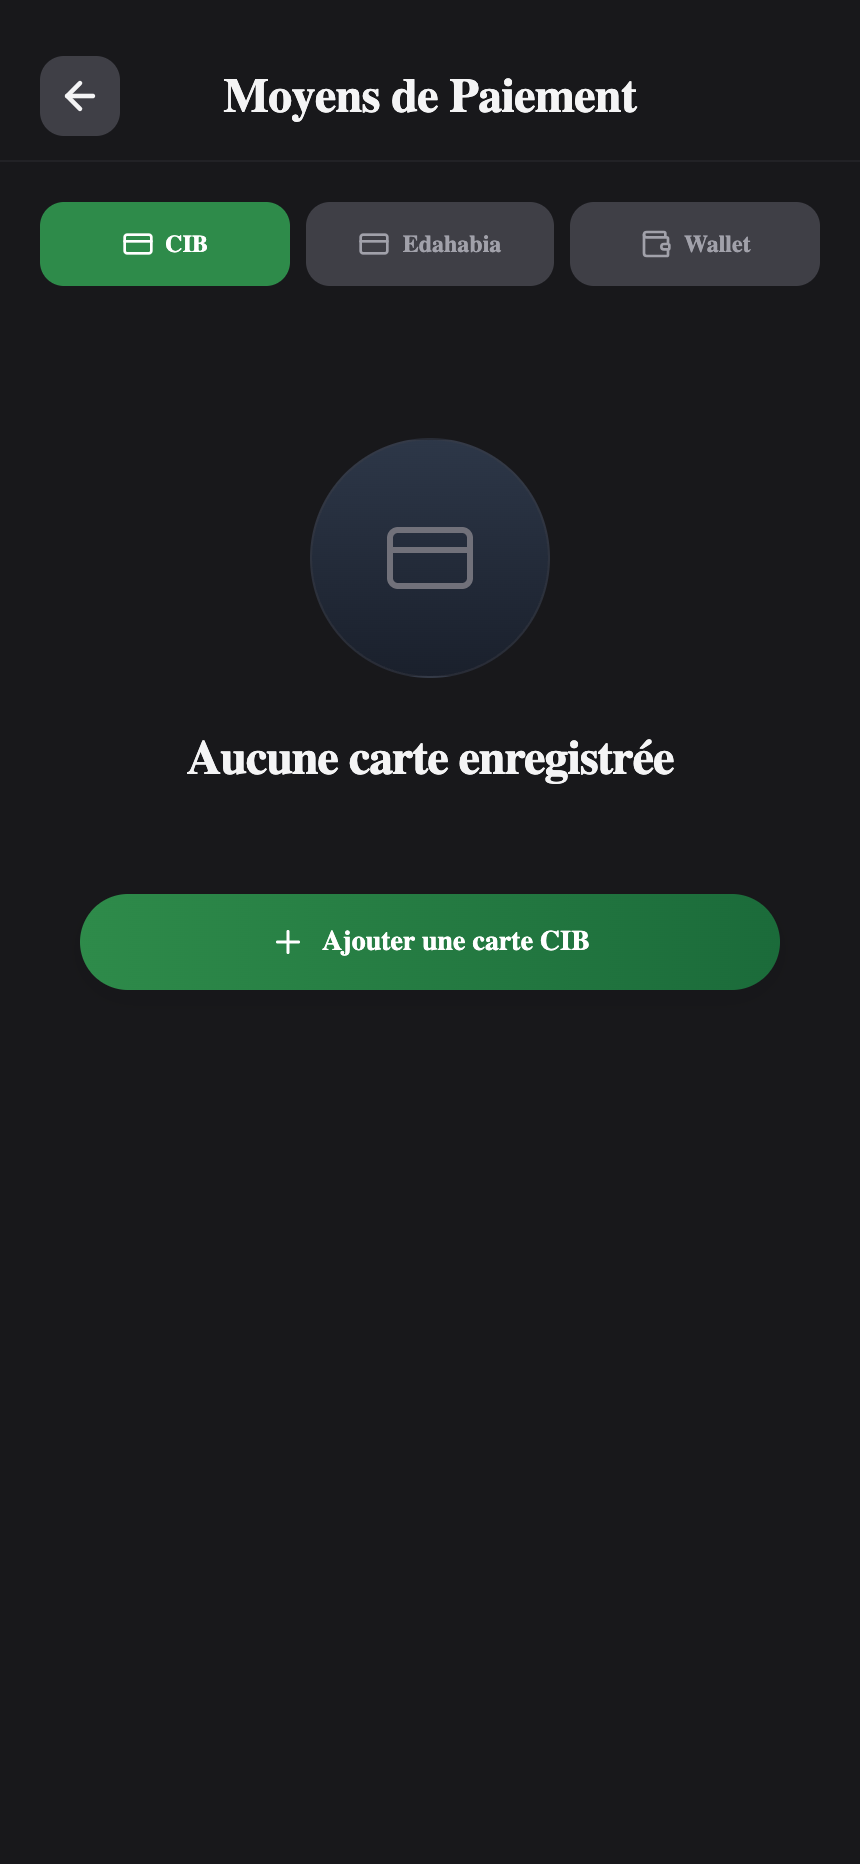
\includegraphics[width=\linewidth]{mobile-all/d_16_payment_methods.png}
    {\footnotesize D.47 --- Méthodes de paiement\par}
\end{minipage}\hfill
\begin{minipage}{0.30\textwidth}
    \centering
    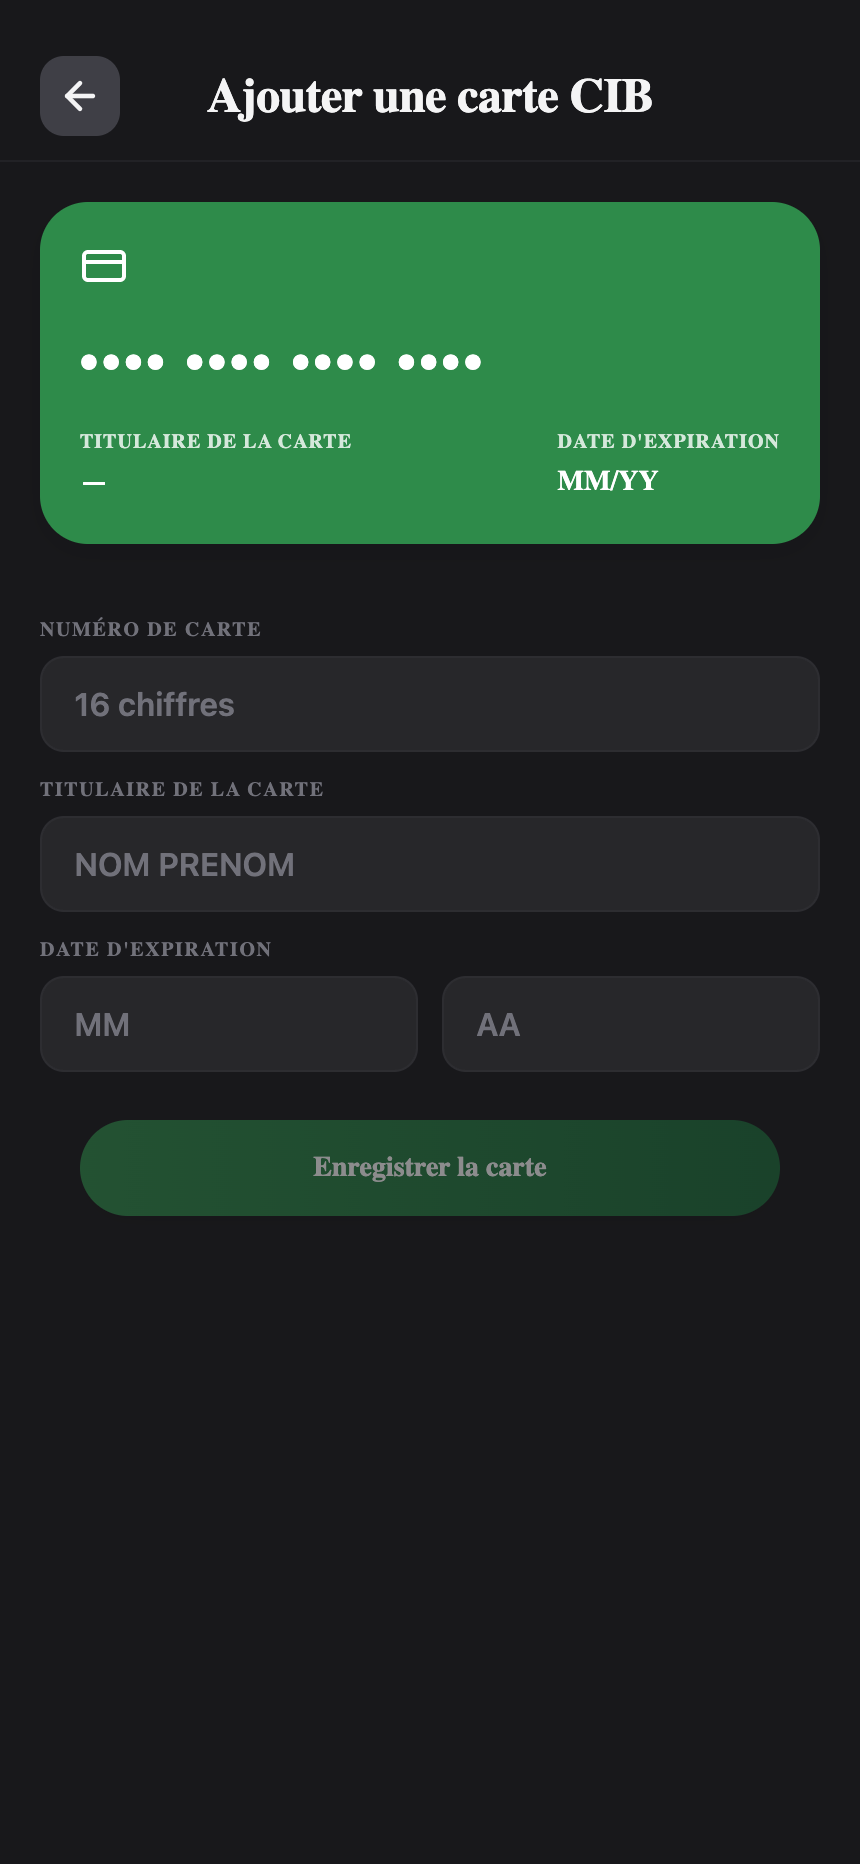
\includegraphics[width=\linewidth]{mobile-all/d_17_add_card.png}
    {\footnotesize D.48 --- Ajout carte bancaire\par}
\end{minipage}\hfill
\begin{minipage}{0.30\textwidth}
    \centering
    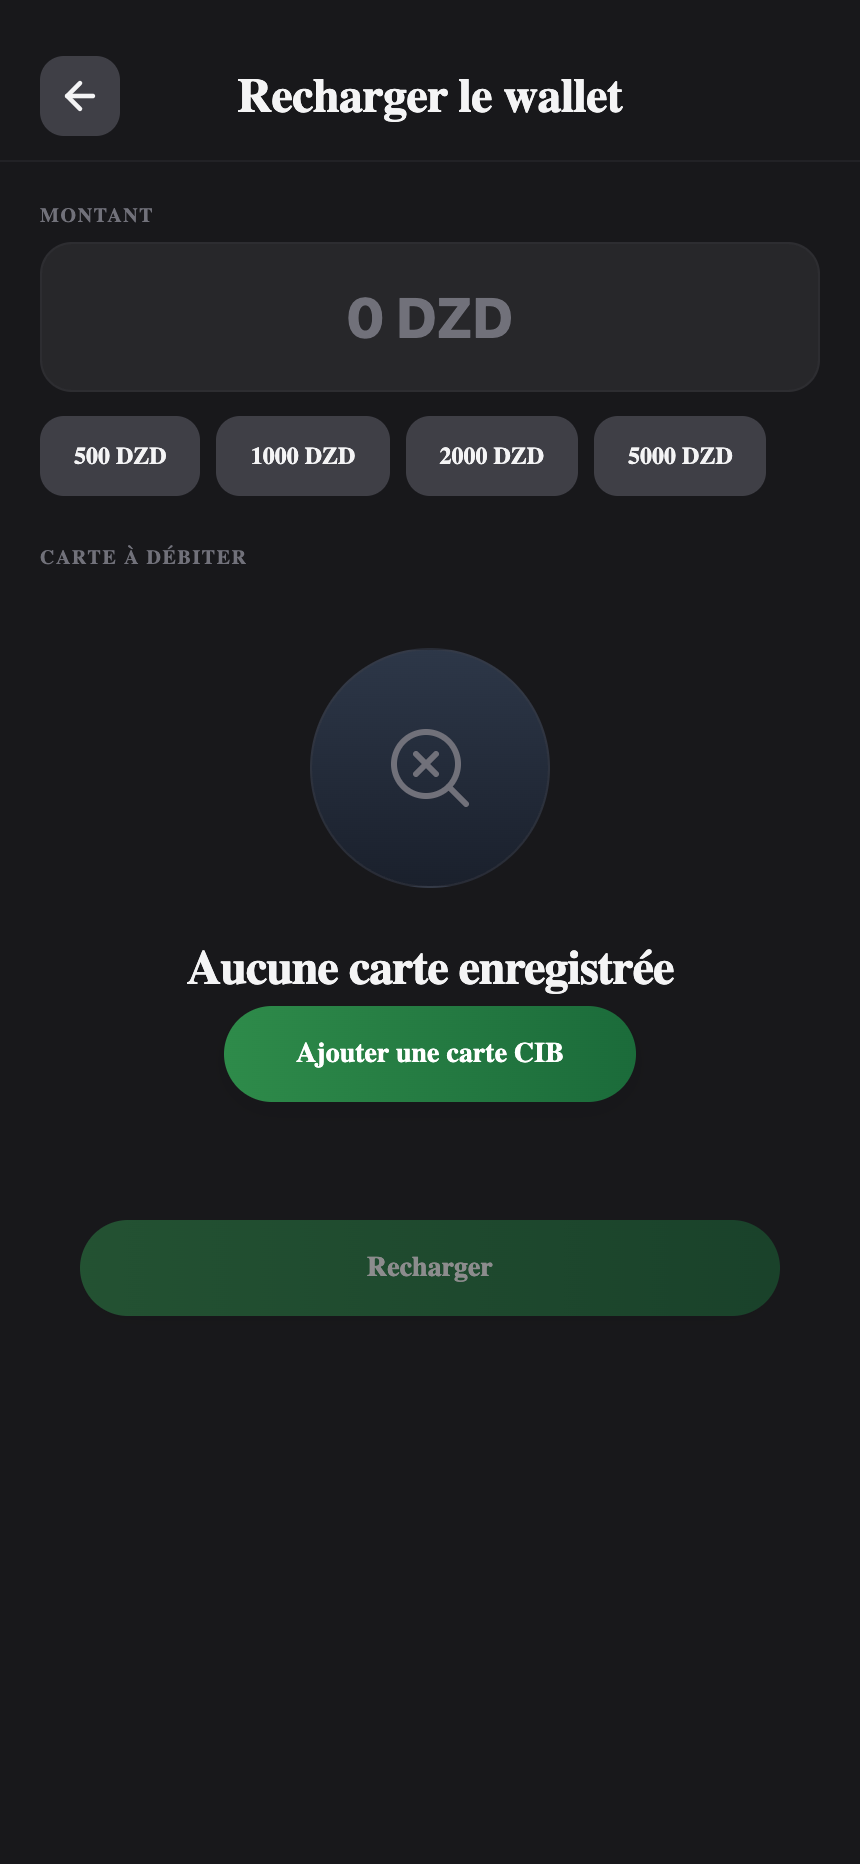
\includegraphics[width=\linewidth]{mobile-all/d_18_wallet_recharge.png}
    {\footnotesize D.49 --- Recharge portefeuille\par}
\end{minipage}
\end{figure}

\begin{figure}[H]
\centering
\begin{minipage}{0.30\textwidth}
    \centering
    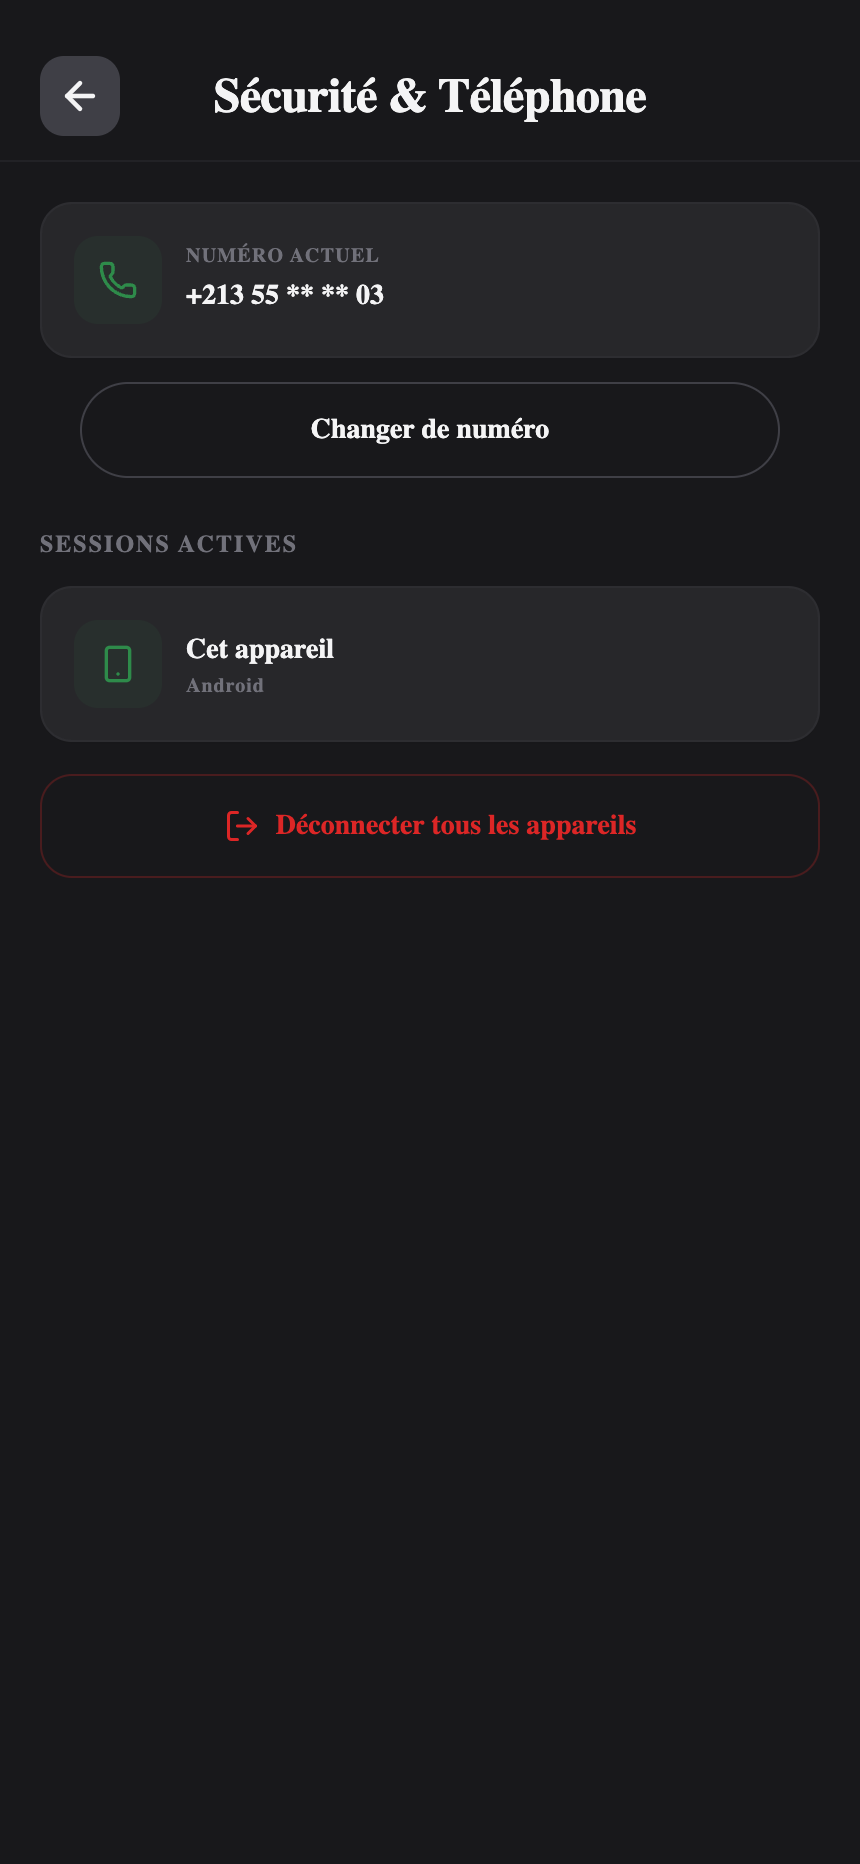
\includegraphics[width=\linewidth]{mobile-all/d_19_security_phone.png}
    {\footnotesize D.50 --- Sécurité du compte\par}
\end{minipage}\hfill
\begin{minipage}{0.30\textwidth}
    \centering
    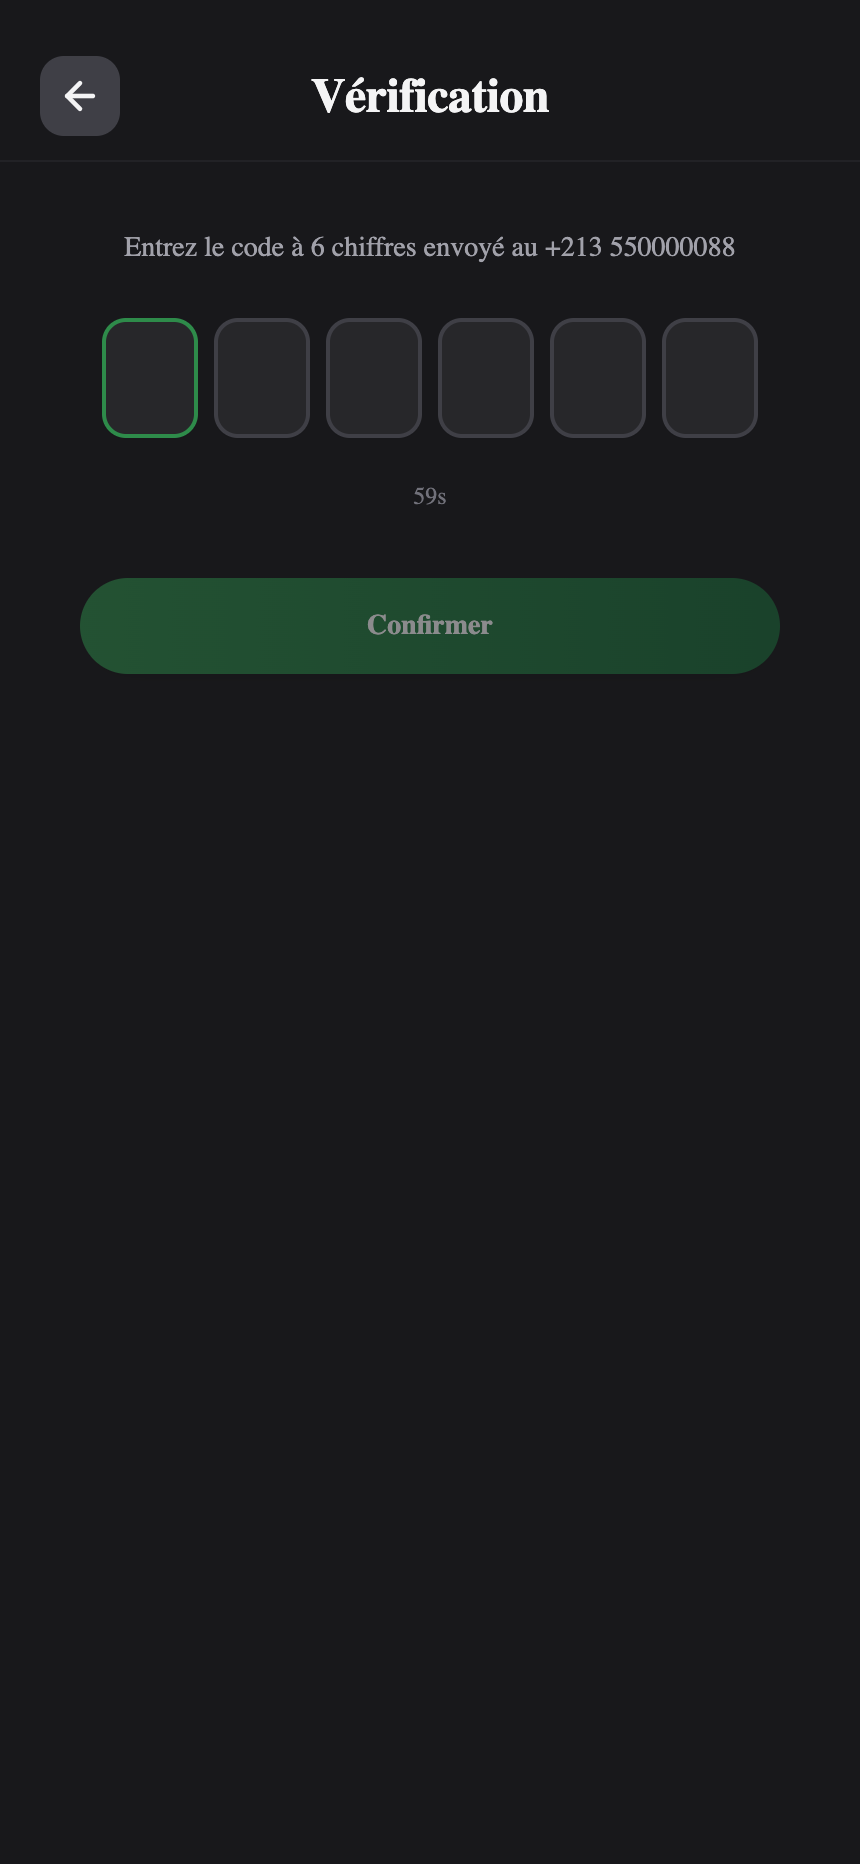
\includegraphics[width=\linewidth]{mobile-all/d_20_change_phone_otp.png}
    {\footnotesize D.51 --- Changement numéro OTP\par}
\end{minipage}\hfill
\begin{minipage}{0.30\textwidth}
    \centering
    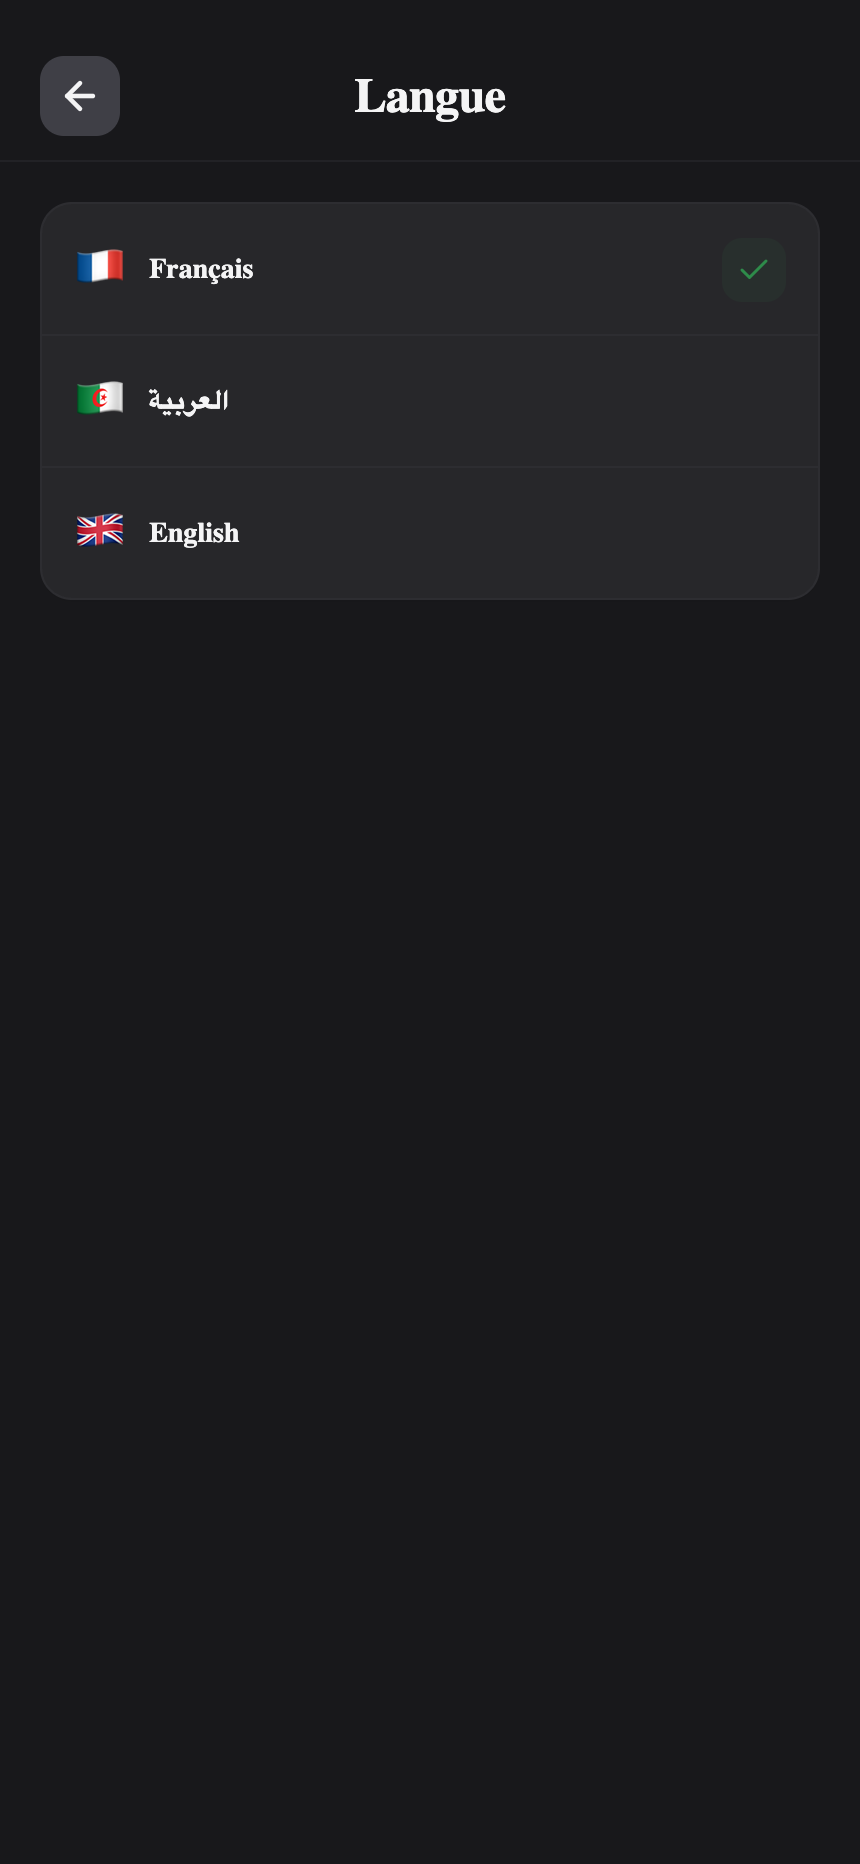
\includegraphics[width=\linewidth]{mobile-all/d_21_language_select.png}
    {\footnotesize D.52 --- Sélection langue\par}
\end{minipage}
\end{figure}

\begin{figure}[H]
\centering
\begin{minipage}{0.30\textwidth}
    \centering
    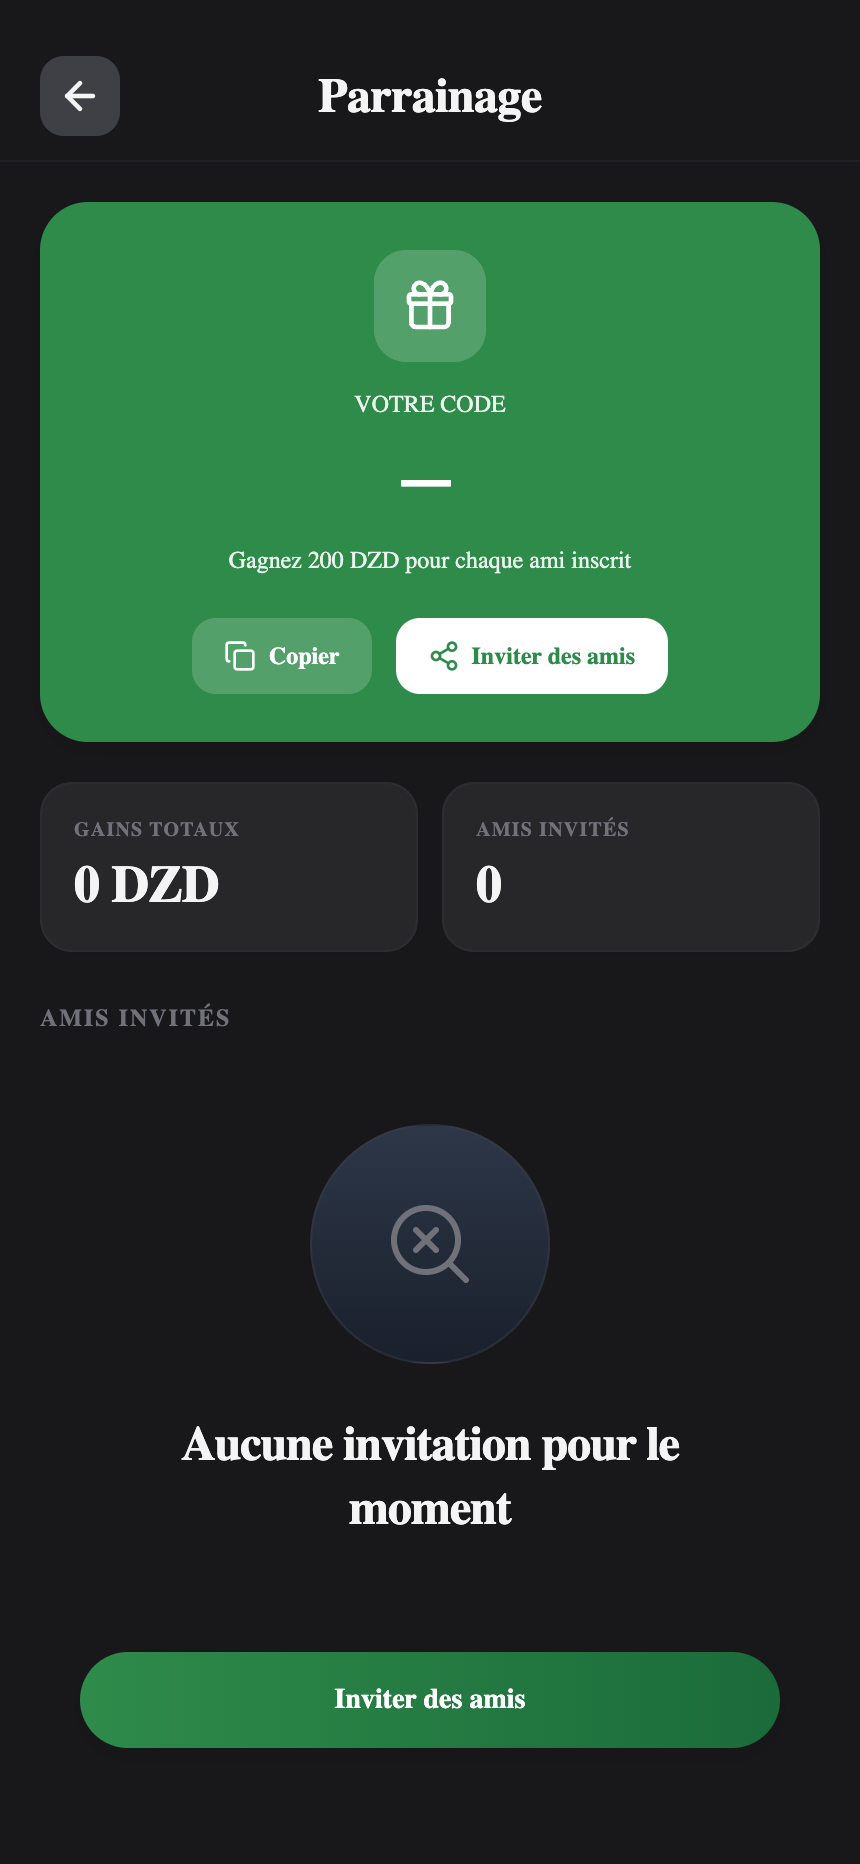
\includegraphics[width=\linewidth]{mobile-all/d_22_referral.png}
    {\footnotesize D.53 --- Parrainage\par}
\end{minipage}\hfill
\begin{minipage}{0.30\textwidth}
    \centering
    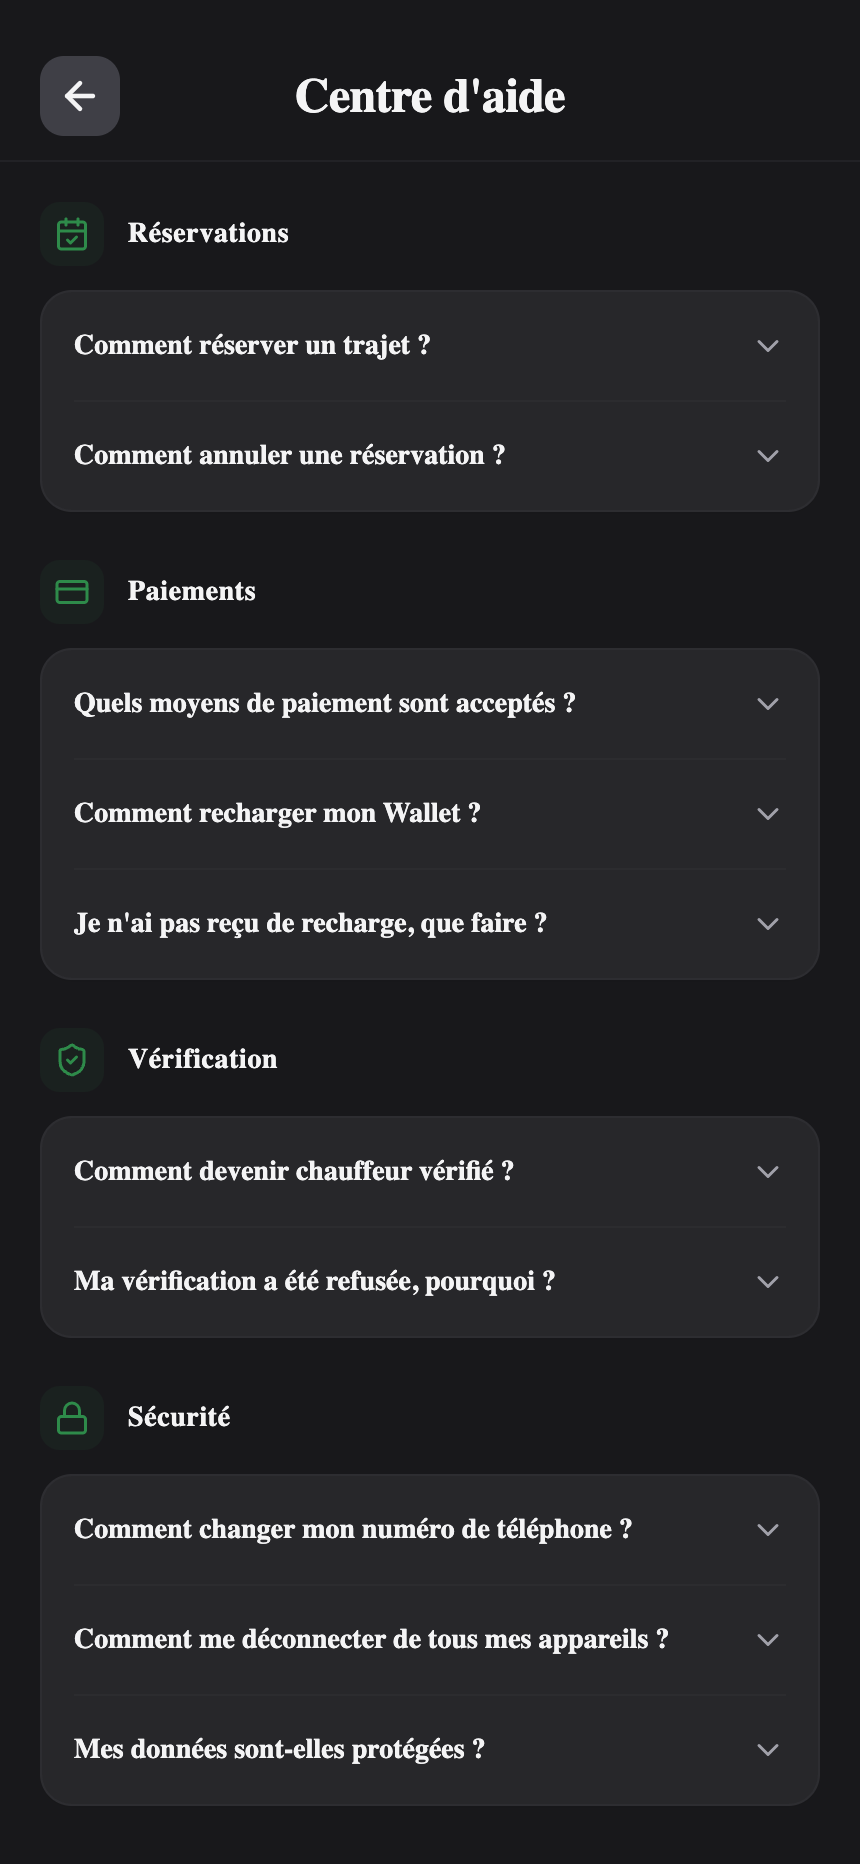
\includegraphics[width=\linewidth]{mobile-all/d_23_help_center.png}
    {\footnotesize D.54 --- Centre d'aide\par}
\end{minipage}\hfill
\begin{minipage}{0.30\textwidth}
    \centering
    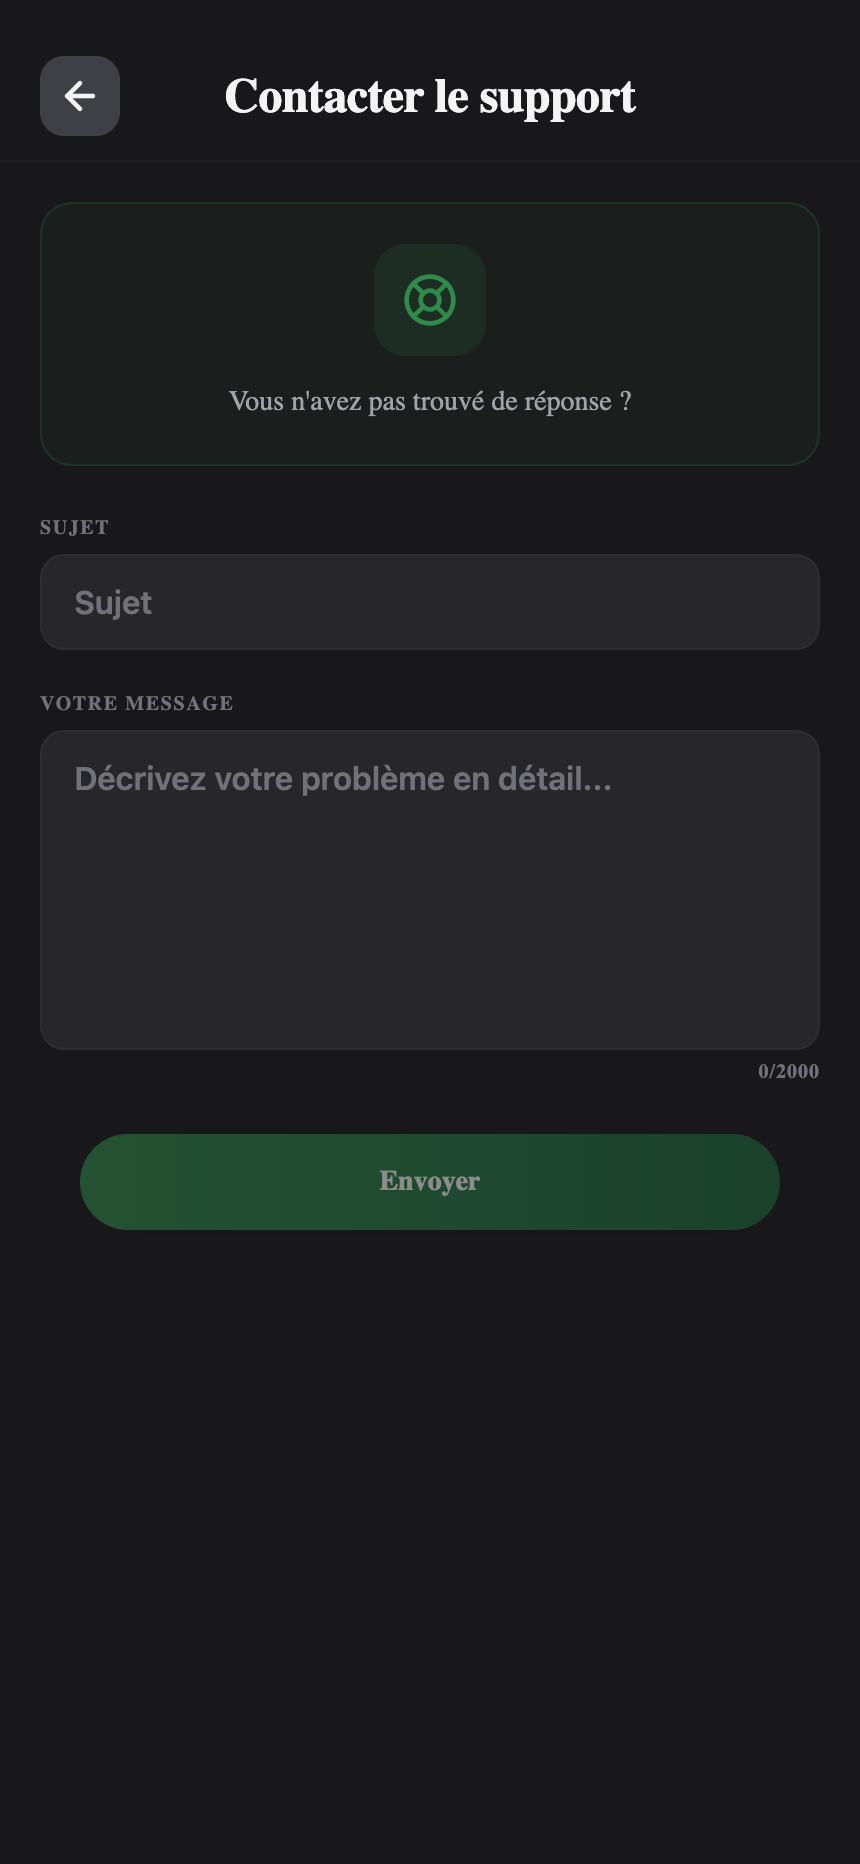
\includegraphics[width=\linewidth]{mobile-all/d_24_contact_support.png}
    {\footnotesize D.55 --- Contacter le support\par}
\end{minipage}
\end{figure}

\begin{figure}[H]
\centering
\begin{minipage}{0.30\textwidth}
    \centering
    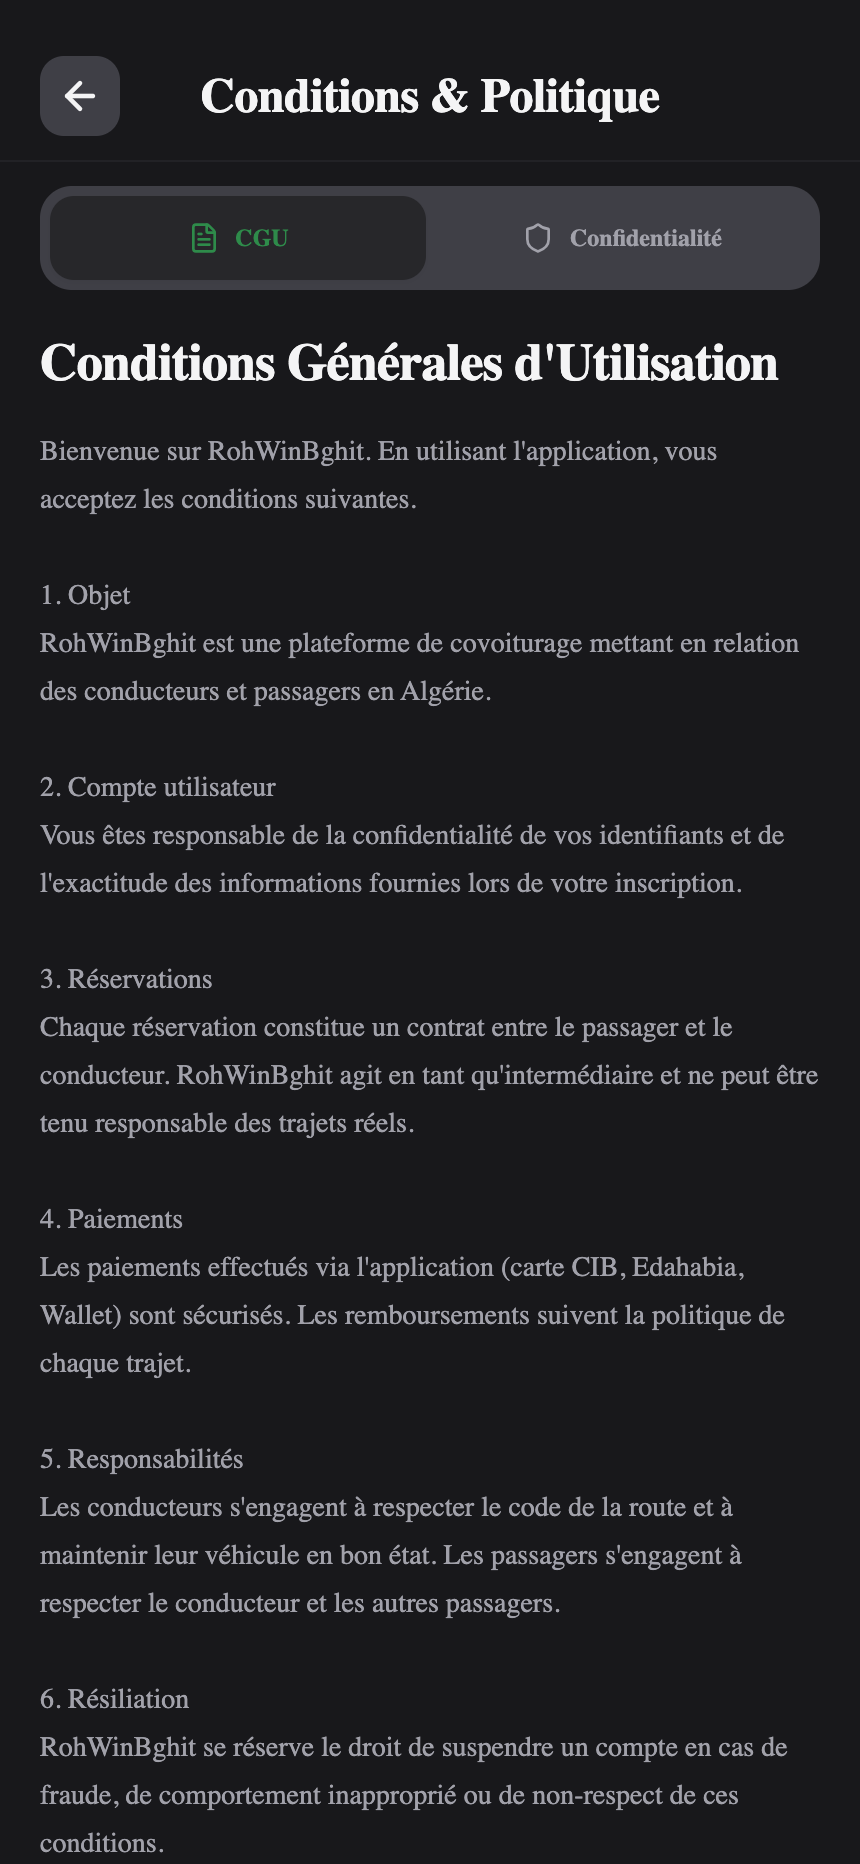
\includegraphics[width=\linewidth]{mobile-all/d_25_terms_legal.png}
    {\footnotesize D.56 --- CGU et confidentialité\par}
\end{minipage}\hfill
\begin{minipage}{0.30\textwidth}
    \centering
    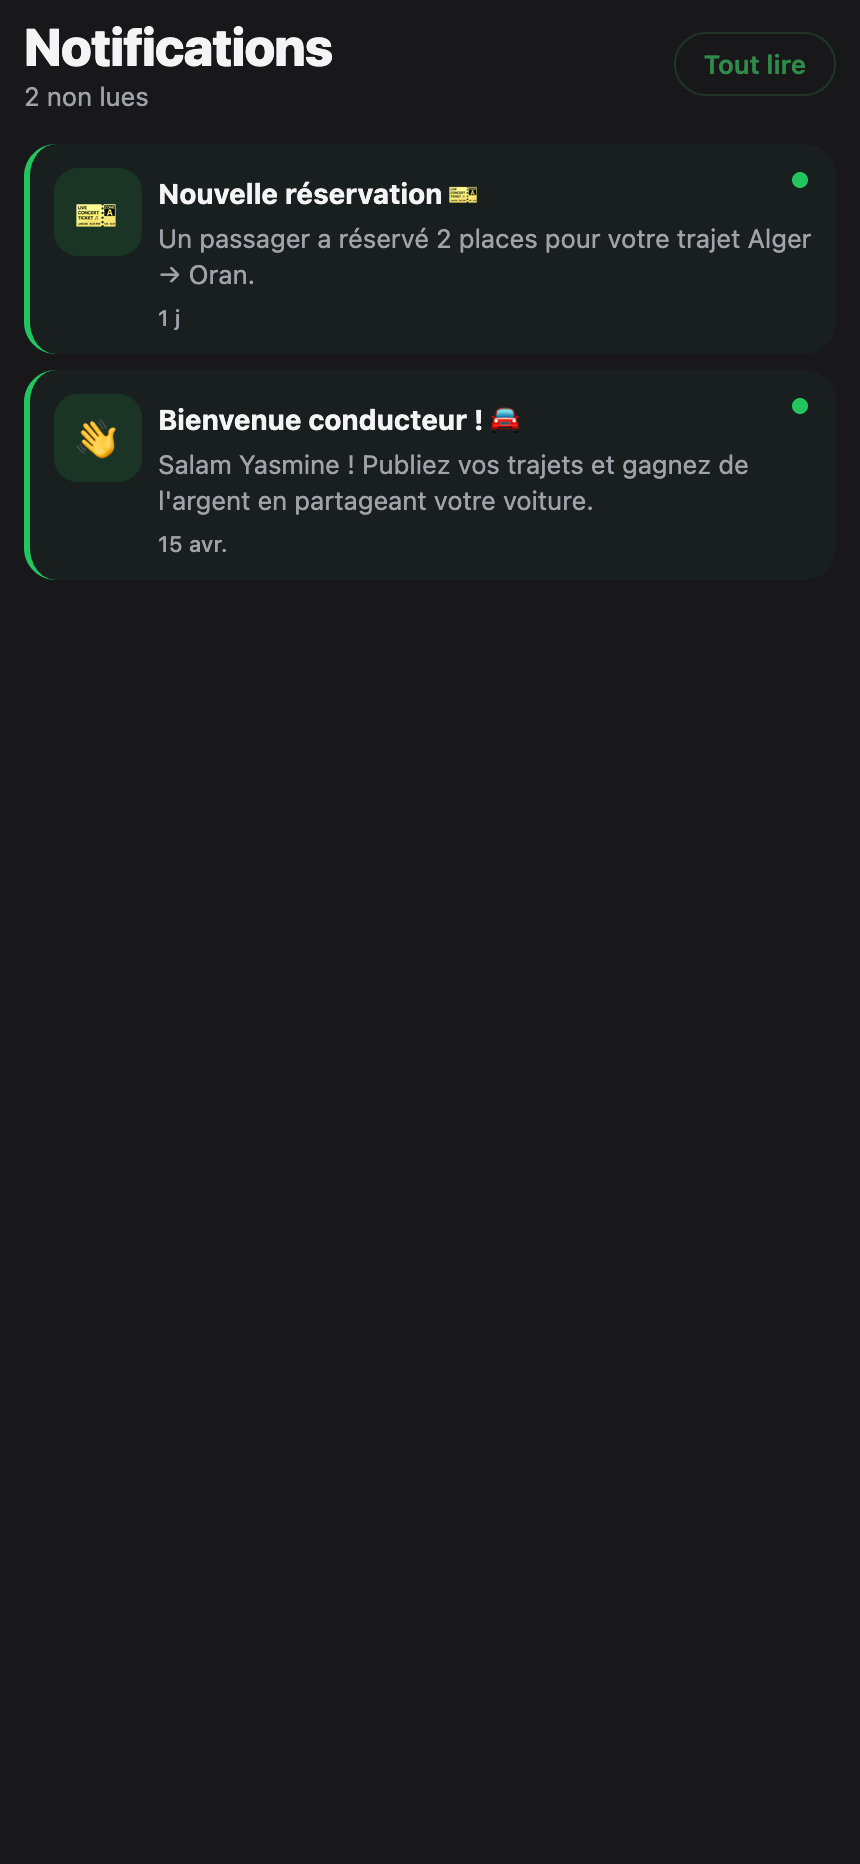
\includegraphics[width=\linewidth]{mobile-all/d_26_notifications.png}
    {\footnotesize D.57 --- Préf. notifications\par}
\end{minipage}\hfill
\begin{minipage}{0.30\textwidth}
    \centering
    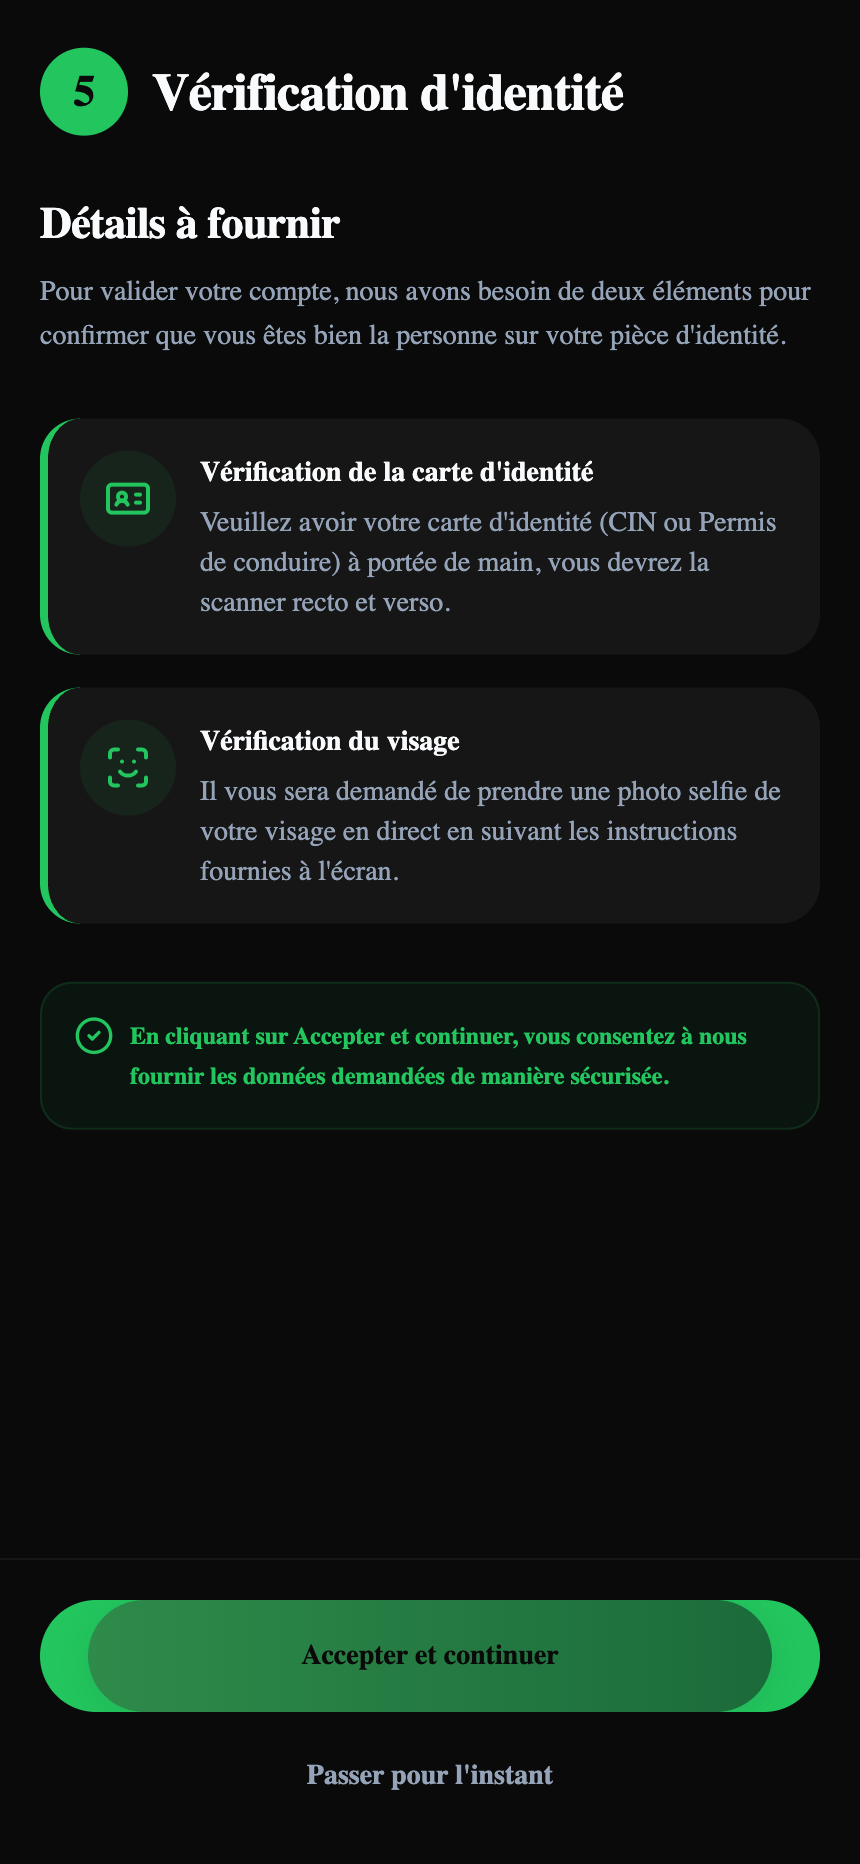
\includegraphics[width=\linewidth]{mobile-all/d_27_verif_intro.png}
    {\footnotesize D.58 --- Introduction KYC\par}
\end{minipage}
\end{figure}

\begin{figure}[H]
\centering
\begin{minipage}{0.30\textwidth}
    \centering
    
\includegraphics[width=\linewidth]{mobile-all/d_28_verif_id_capture.png}
    {\footnotesize D.59 --- Capture CIN\par}
\end{minipage}\hfill
\begin{minipage}{0.30\textwidth}
    \centering
    
\includegraphics[width=\linewidth]{mobile-all/d_29_verif_face_capture.png}
    {\footnotesize D.60 --- Capture vivacité\par}
\end{minipage}\hfill
\begin{minipage}{0.30\textwidth}
    \centering
    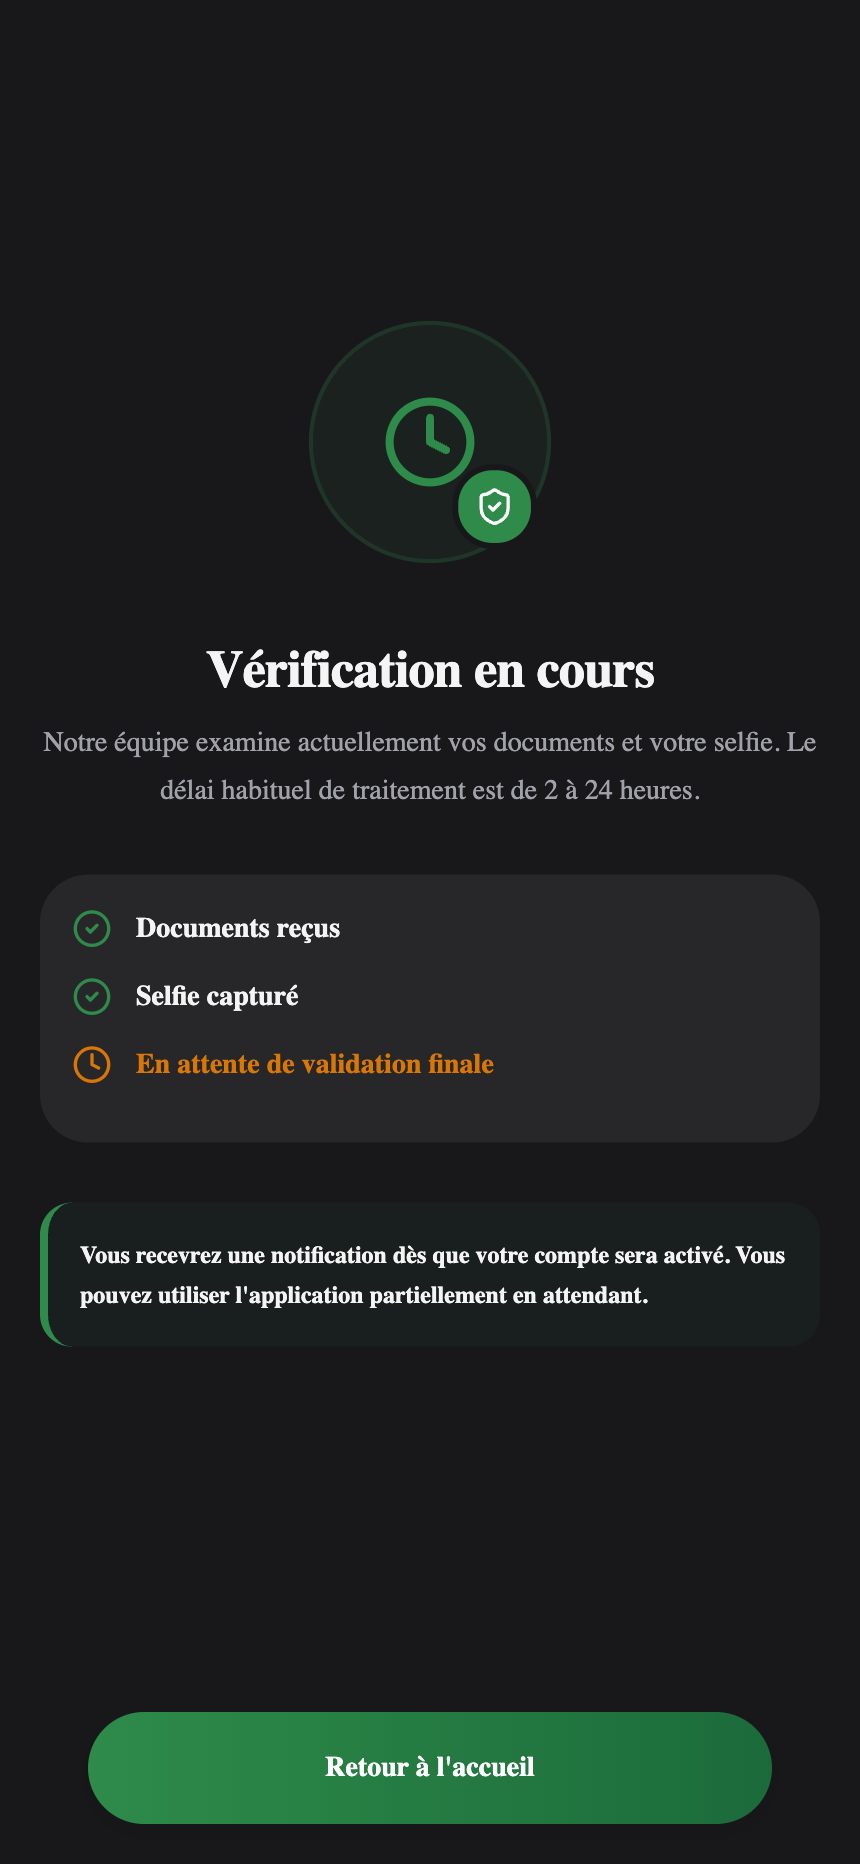
\includegraphics[width=\linewidth]{mobile-all/d_30_verif_pending.png}
    {\footnotesize D.61 --- KYC en attente\par}
\end{minipage}
\end{figure}

\begin{figure}[H]
\centering
\begin{minipage}{0.30\textwidth}
    \centering
    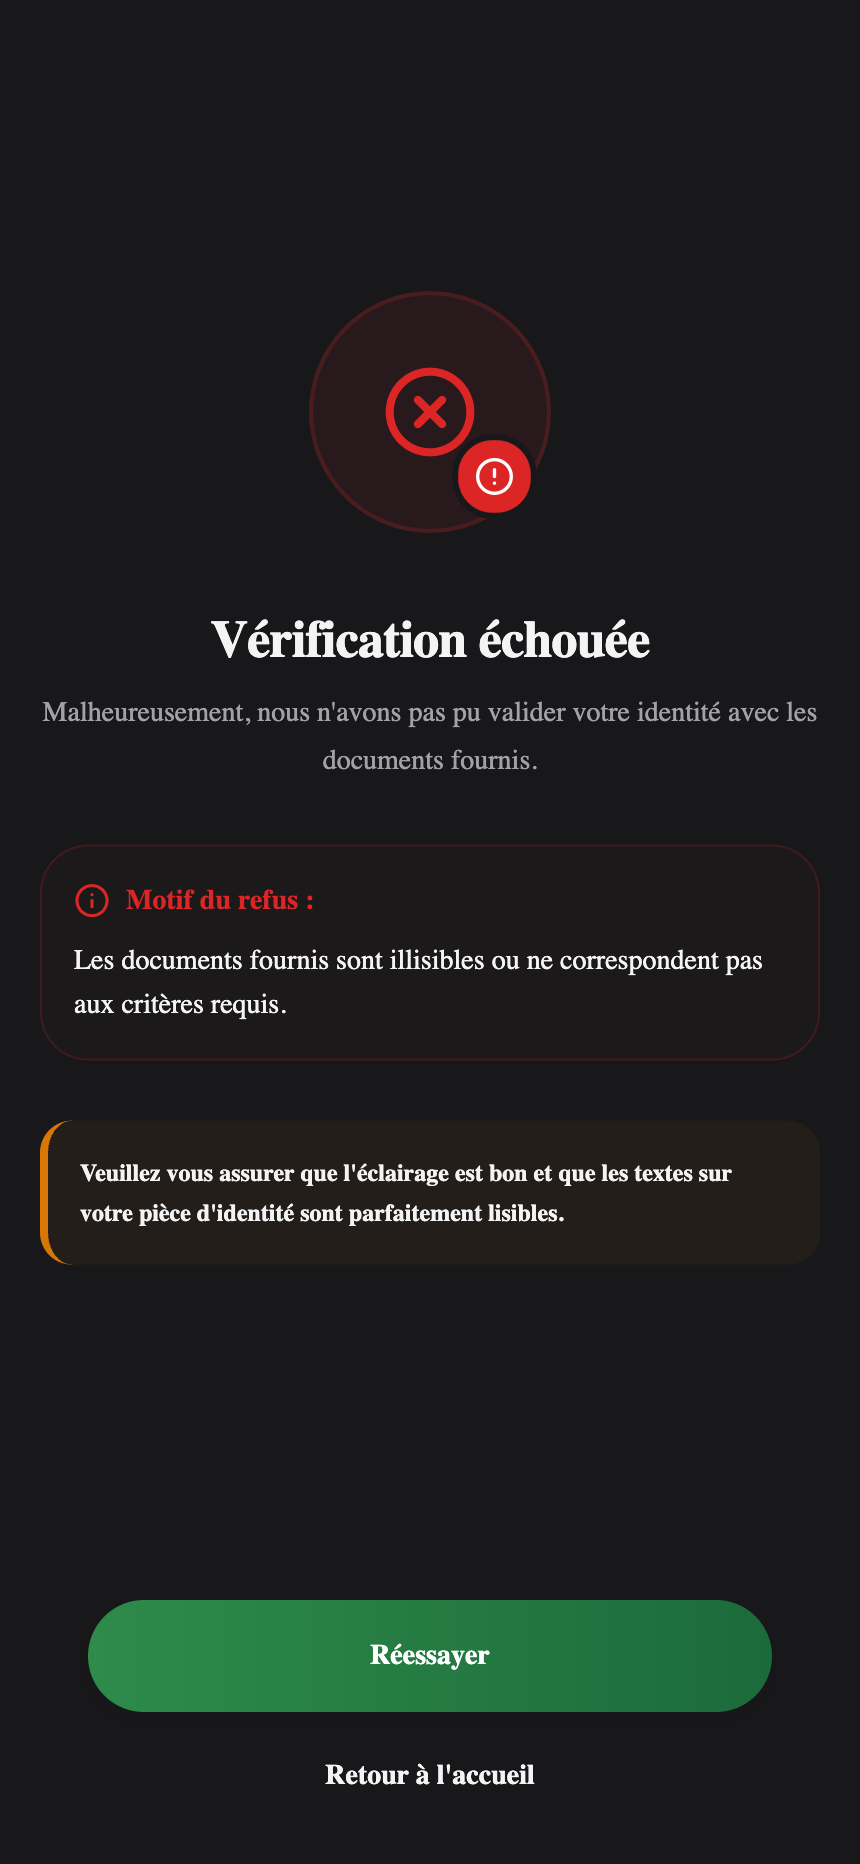
\includegraphics[width=\linewidth]{mobile-all/d_31_verif_rejected.png}
    {\footnotesize D.62 --- KYC rejeté (conducteur)\par}
\end{minipage}
\caption{Interfaces conducteur --- Écrans D.32 à D.62}
\end{figure}

% ----------------------------------------------------------------
\section{Panneau d'administration}
% ----------------------------------------------------------------

\begin{figure}[H]
\centering
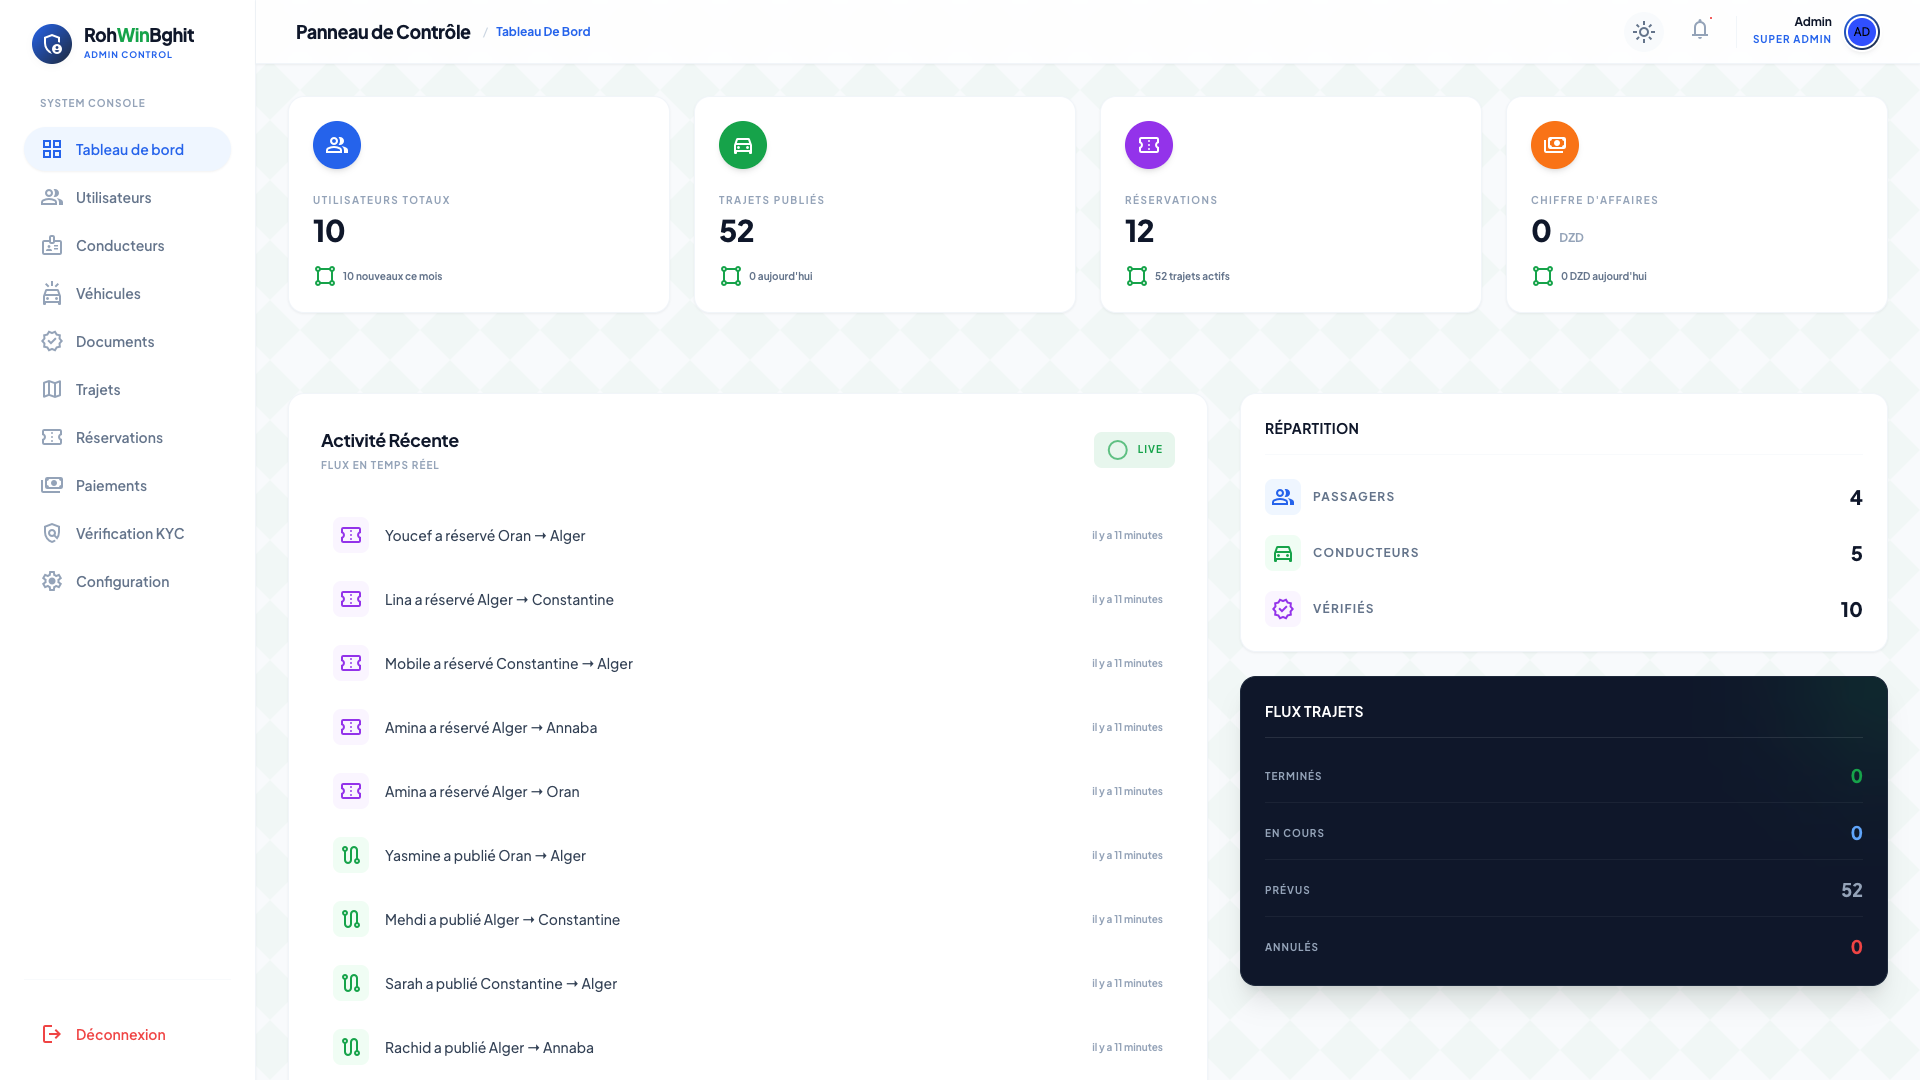
\includegraphics[width=0.9\linewidth]{assets/admin_dashboard.png}
\caption{D.63 --- Tableau de bord central de l'administration}
\end{figure}

\begin{figure}[H]
\centering
\begin{minipage}{0.48\textwidth}
    \centering
    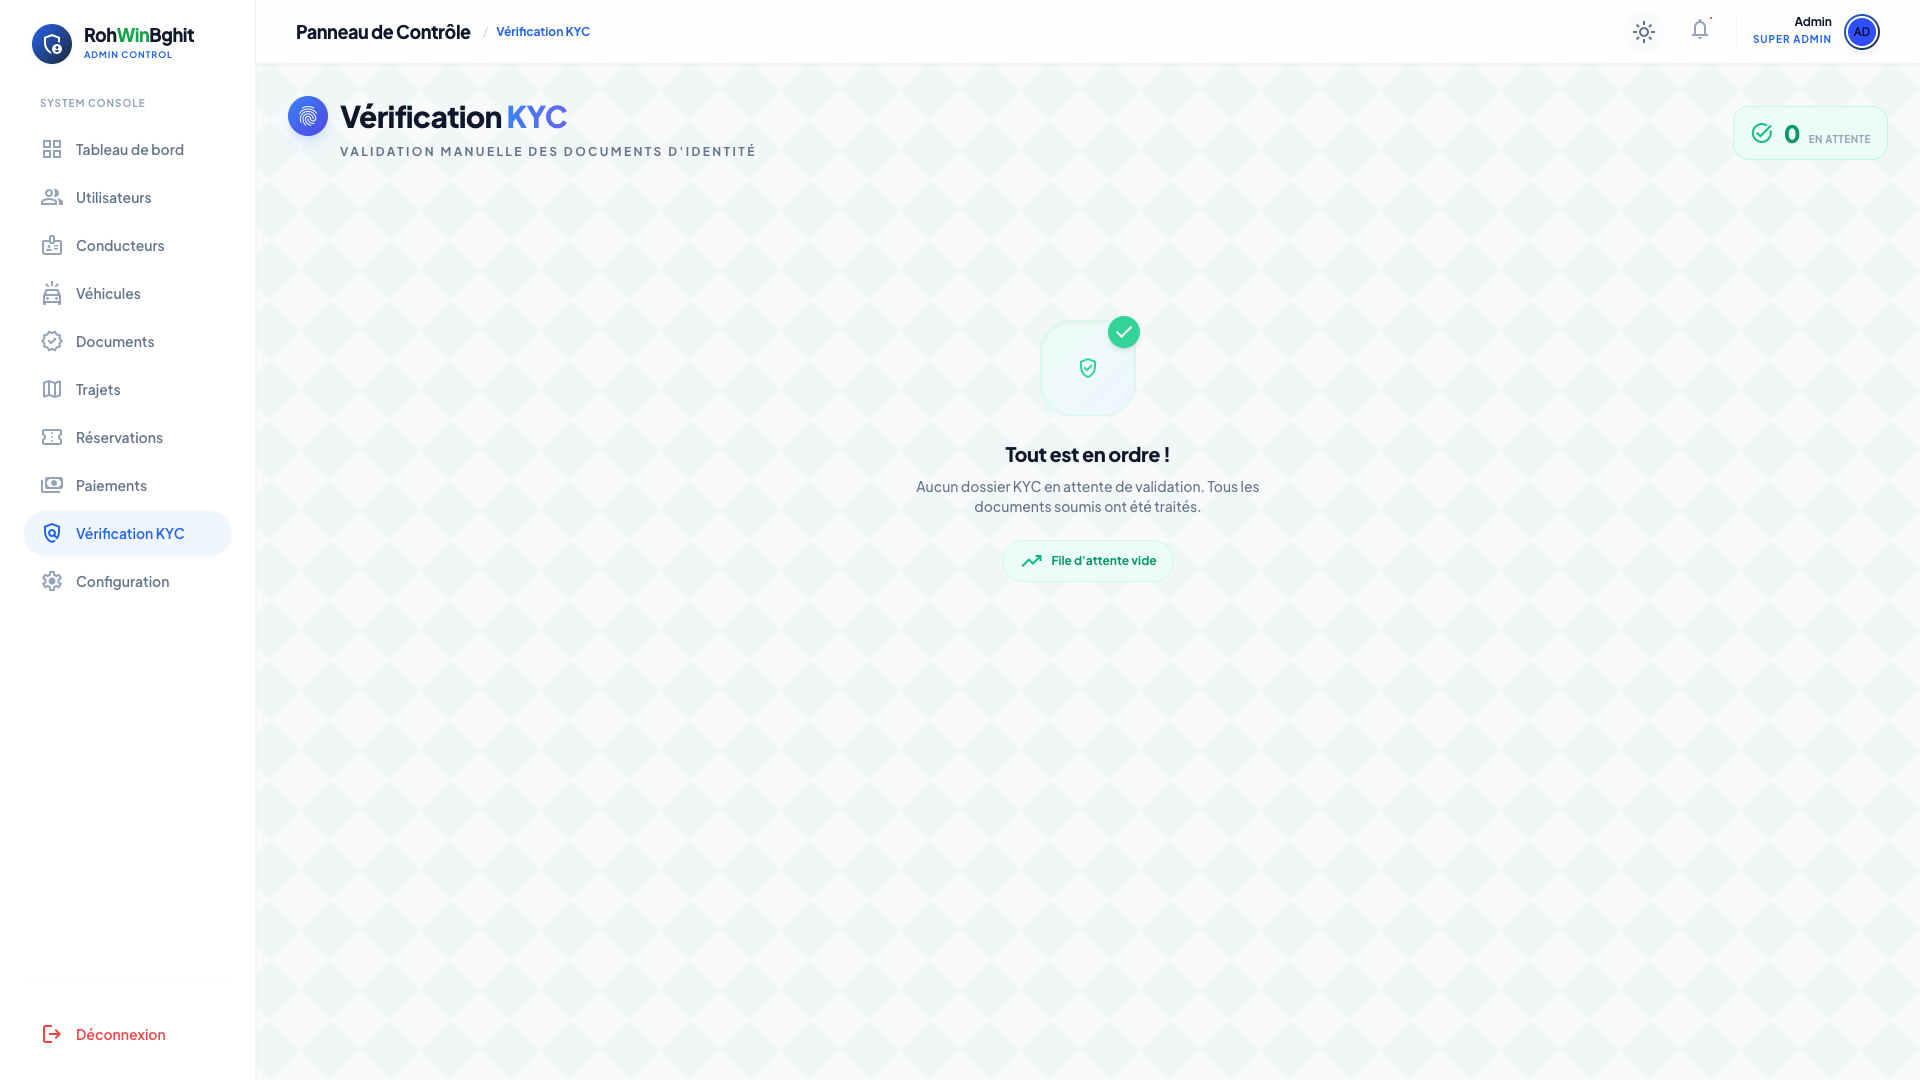
\includegraphics[width=\linewidth]{assets/admin_kyc.png}
    {\footnotesize D.64 --- Revue manuelle des dossiers KYC\par}
\end{minipage}\hfill
\begin{minipage}{0.48\textwidth}
    \centering
    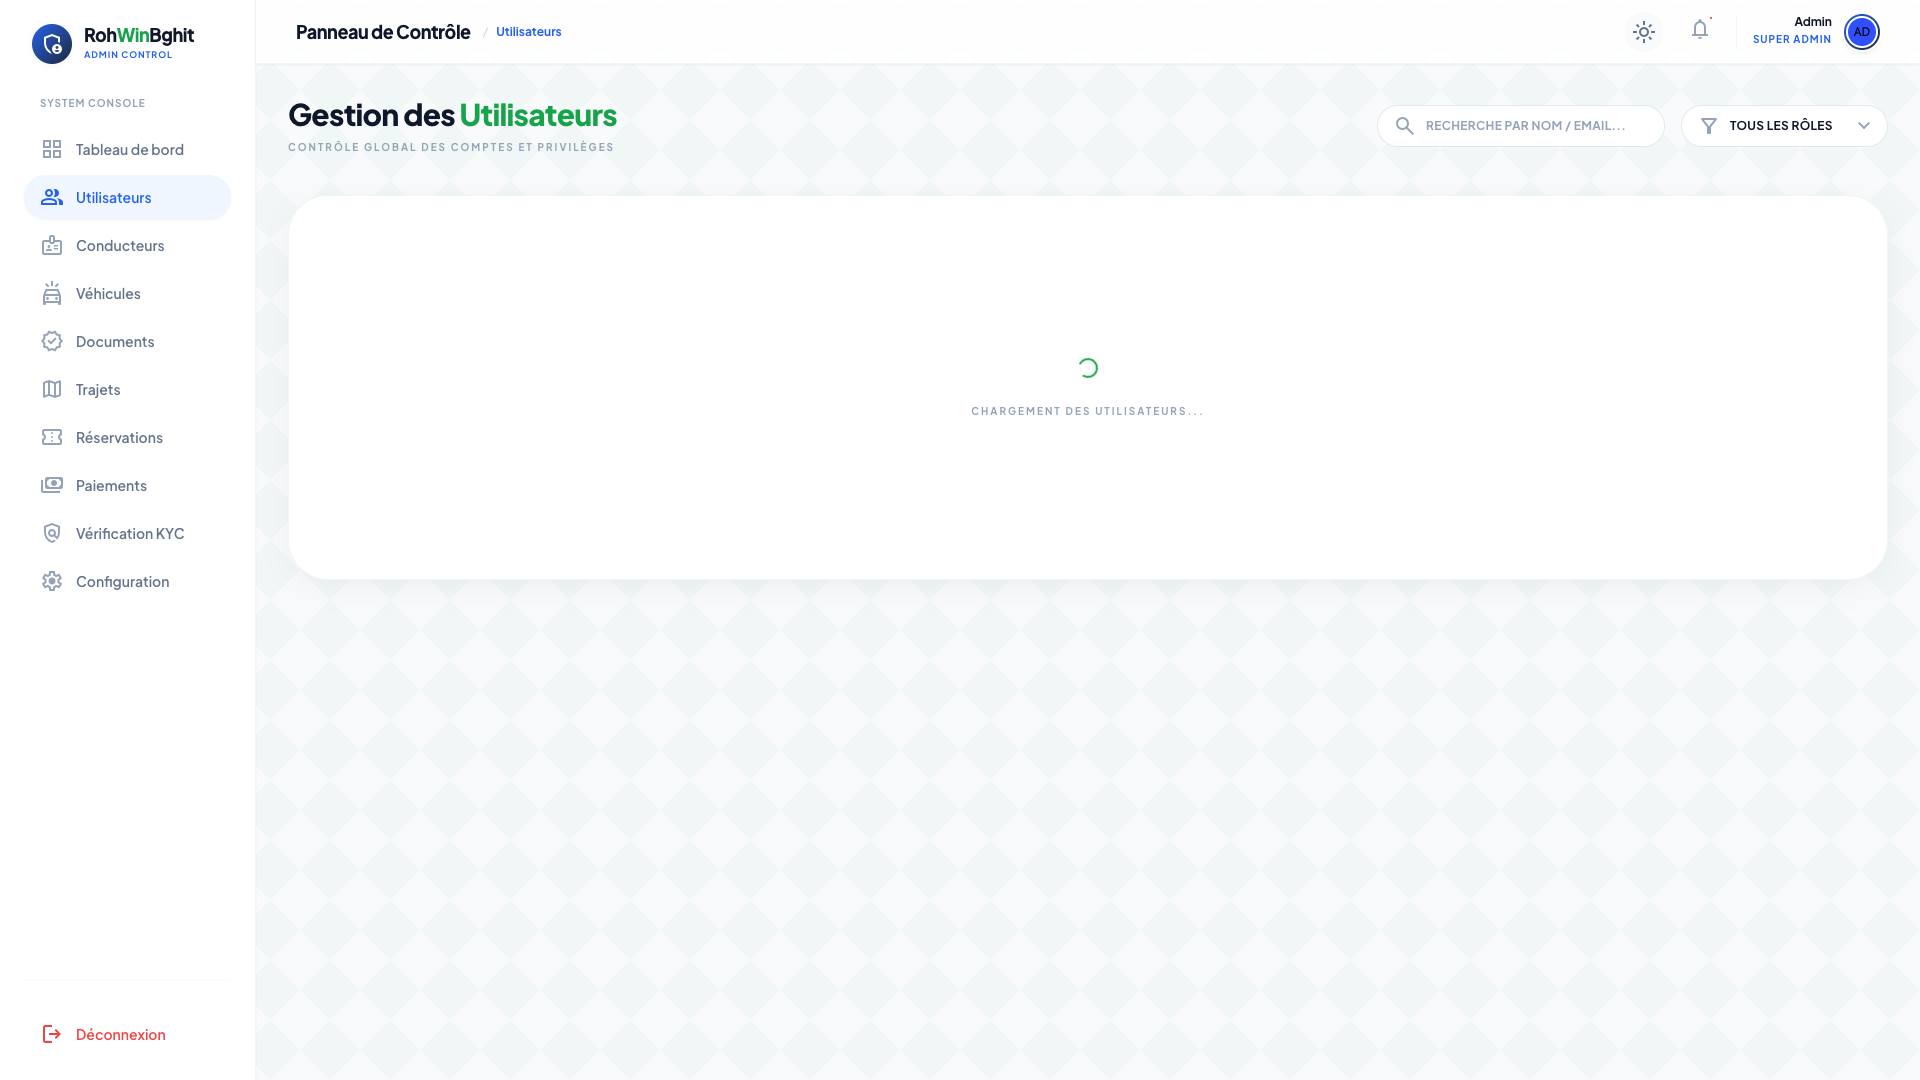
\includegraphics[width=\linewidth]{assets/admin_users.png}
    {\footnotesize D.65 --- Gestion des utilisateurs\par}
\end{minipage}
\end{figure}

\begin{figure}[H]
\centering
\begin{minipage}{0.48\textwidth}
    \centering
    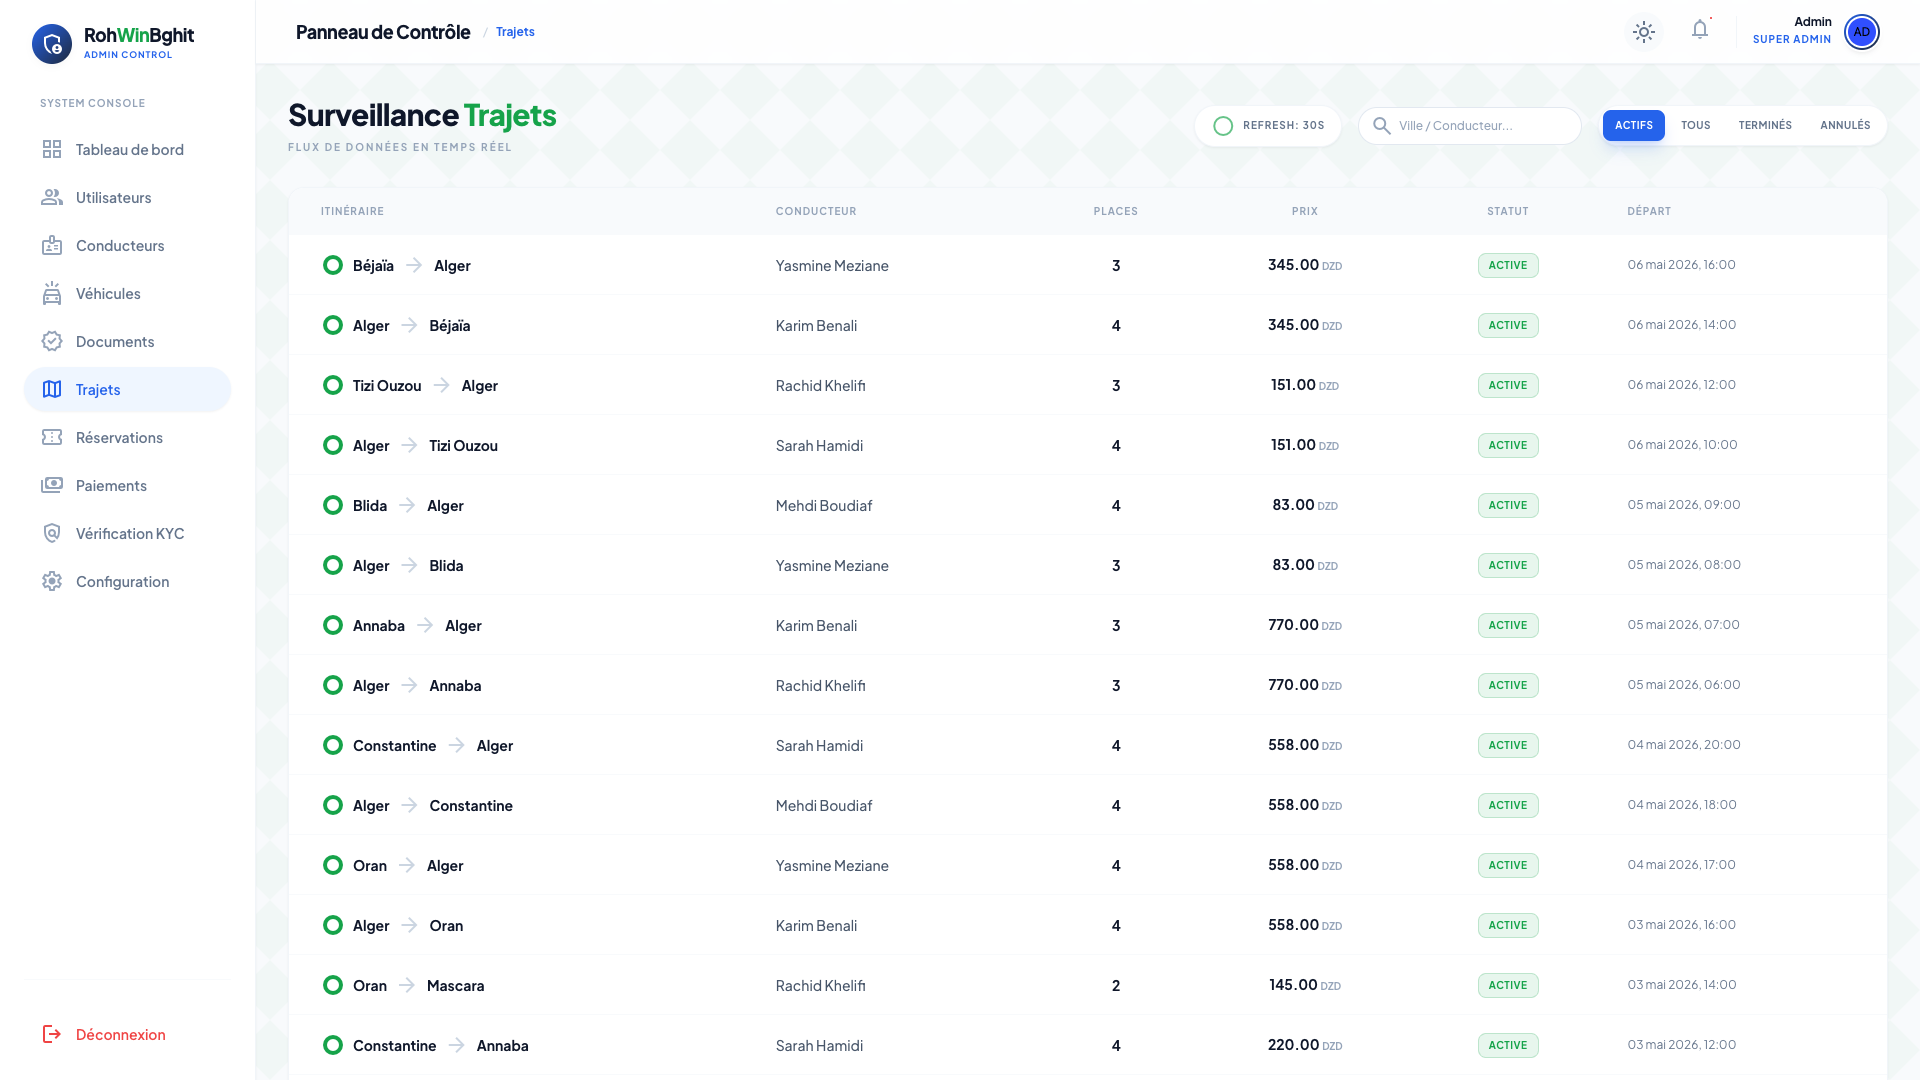
\includegraphics[width=\linewidth]{assets/admin_trips.png}
    {\footnotesize D.66 --- Supervision des trajets\par}
\end{minipage}\hfill
\begin{minipage}{0.48\textwidth}
    \centering
    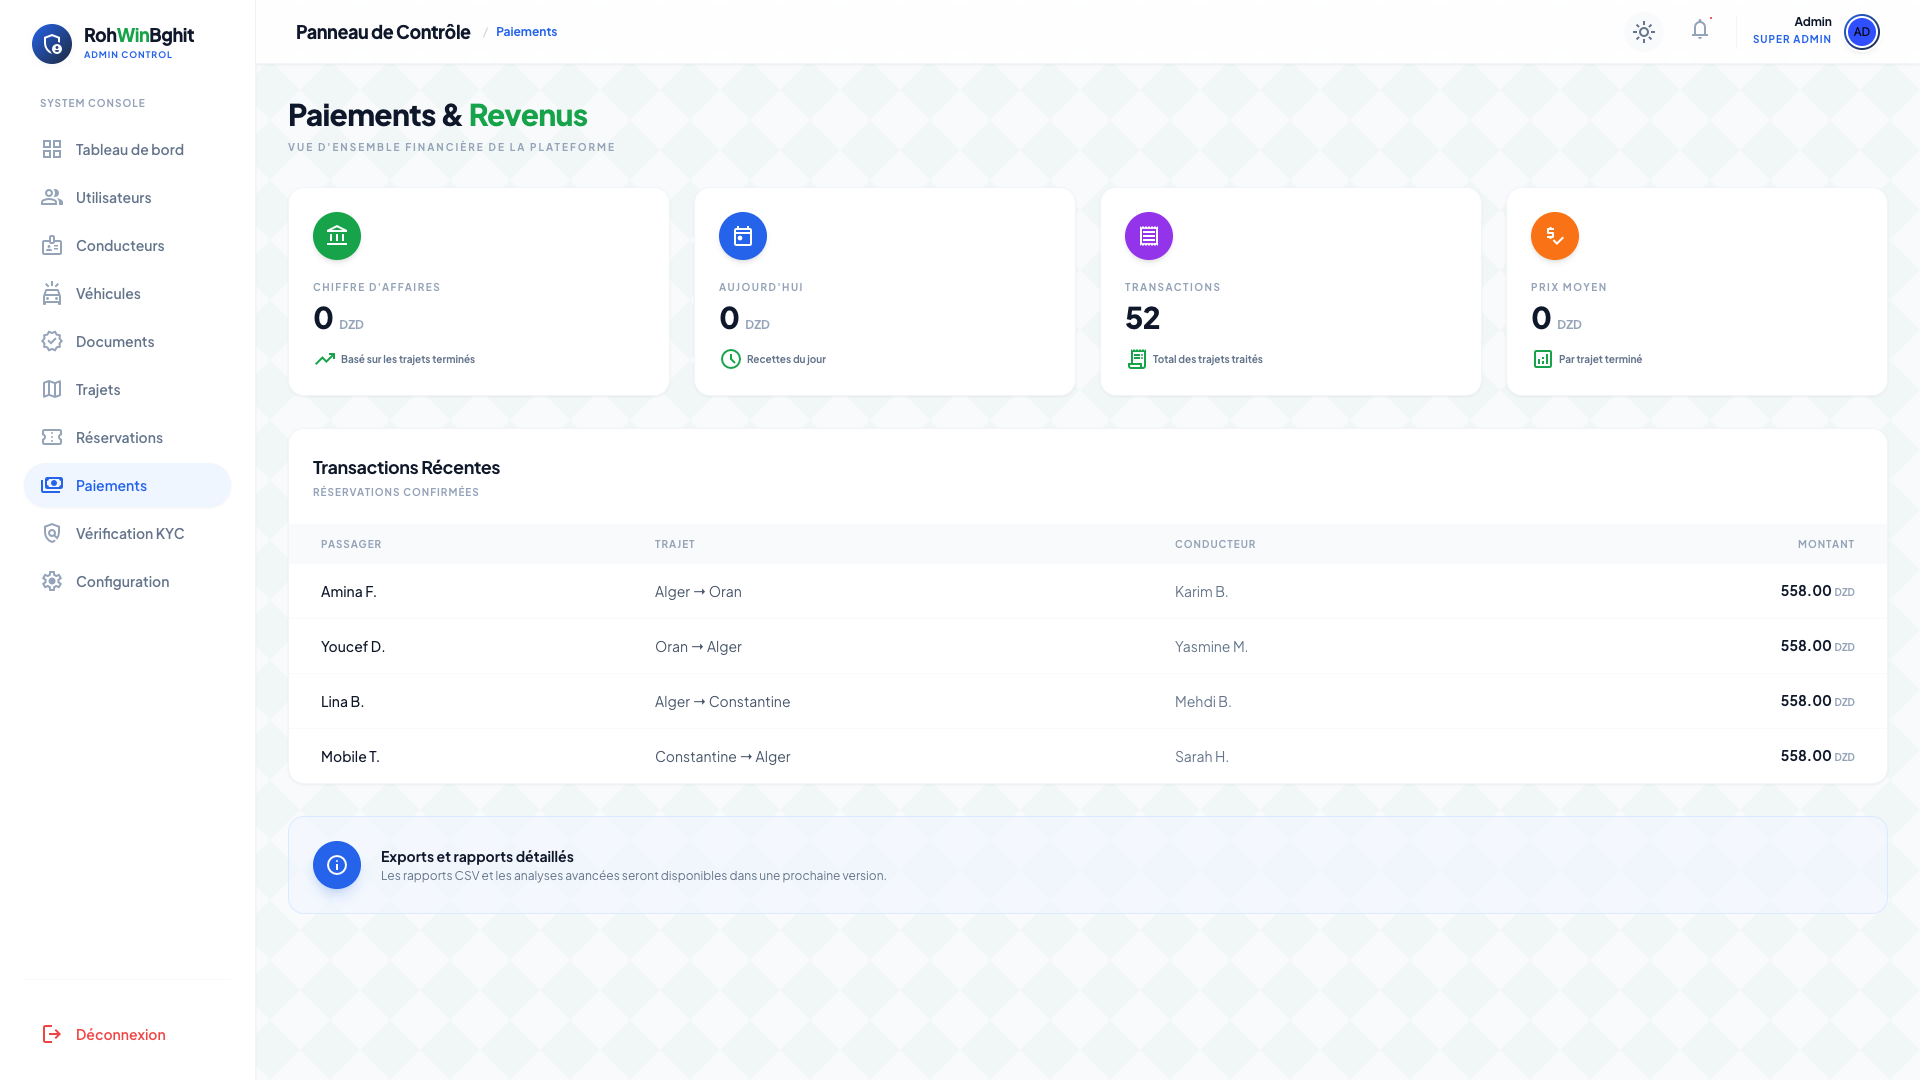
\includegraphics[width=\linewidth]{assets/admin_payments.png}
    {\footnotesize D.67 --- Suivi des transactions\par}
\end{minipage}
\caption{Panneau d'administration --- Captures D.63 à D.67}
\end{figure}


\section*{Annexe D — Scénarios de tests}
\addcontentsline{toc}{section}{Annexe D — Scénarios de tests}
\label{annexe:tests}

Cette annexe récapitule les scénarios de tests exécutés pour valider le fonctionnement de la plateforme.

\begin{enumerate}
  \item \textbf{Test d'inscription passager :} Saisie de données valides, envoi de l'OTP, validation. (Statut : \textbf{Succès})
  \item \textbf{Test de vérification KYC biométrique :} Envoi de photos floues ou usurpées. Le microservice FastAPI doit rejeter la demande. (Statut : \textbf{Succès})
  \item \textbf{Test de publication de trajet :} Le conducteur publie un trajet avec wilayas de départ/arrivée. (Statut : \textbf{Succès})
  \item \textbf{Test de réservation de place :} Le passager réserve, le nombre de places disponibles diminue. (Statut : \textbf{Succès})
  \item \textbf{Test de paiement électronique :} Saisie de la carte d'Edahabia fictive dans la sandbox SATIM, validation de la transaction. (Statut : \textbf{Succès})
\end{enumerate}

\chapter{Manuel utilisateur}
\label{annexe:manuel}

Ce manuel a pour but de guider les utilisateurs (passagers et conducteurs) ainsi que les administrateurs de la plateforme \textit{RohWinBghit} à travers ses différentes fonctionnalités.

\section{Guide du Passager}
\label{sec:guide-passager}

\subsection{Inscription et connexion}
Lors du premier lancement de l'application, vous devez créer votre compte. Saisissez votre numéro de téléphone. Un code de validation à usage unique (OTP) vous est envoyé par SMS. Après sa saisie et sa validation, complétez vos informations de profil (nom, prénom et adresse email). Pour les connexions ultérieures, la saisie du numéro de téléphone et la validation par SMS sont requises pour garantir la sécurité.

\subsection{Vérification d'identité (KYC)}
Pour pouvoir réserver un trajet, vous devez obligatoirement valider votre identité. Accédez à votre profil et sélectionnez « Vérification d'identité ».
\begin{enumerate}
  \item Cadrez le recto de votre Carte d'Identité Nationale (CIN) dans la zone indiquée et déclenchez la capture. Répétez l'opération pour le verso.
  \item Réalisez le selfie vidéo demandé en effectuant les mouvements affichés à l'écran pour prouver votre présence physique (détection de vivacité).
  \item Soumettez le dossier. Le traitement automatique prend moins de deux minutes. Si les scores de validation sont insuffisants mais corrects, votre dossier sera réorienté vers une revue manuelle par un administrateur.
\end{enumerate}

\subsection{Recherche et réservation}
Sur l'écran d'accueil, indiquez votre wilaya de départ, votre wilaya d'arrivée et la date souhaitée du déplacement. Les résultats s'affichent instantanément. Vous pouvez trier ou filtrer les propositions selon le prix, le niveau de confort du véhicule ou la note du conducteur. Une fois le trajet choisi, sélectionnez le nombre de places et validez votre moyen de paiement (espèces, CIB ou Edahabia).

\subsection{Messagerie et suivi temps réel}
Une fois la réservation confirmée, accédez au chat intégré pour communiquer en toute sécurité avec le conducteur sans divulguer votre numéro de téléphone. Le jour du départ, suivez la position GPS du véhicule en temps réel sur la carte intégrée pour connaître son heure précise d'arrivée (ETA).

\section{Guide du Conducteur}
\label{sec:guide-conducteur}

\subsection{Enregistrement d'un véhicule}
Pour passer en mode conducteur, accédez aux paramètres de votre profil. Enregistrez votre véhicule en renseignant la marque, le modèle, l'année et la couleur. Vous devez téléverser une photo lisible de la plaque d'immatriculation (qui sera chiffrée par AES-256 en base de données) ainsi que vos documents réglementaires (carte grise, assurance en cours de validité et contrôle technique).

\subsection{Publication d'un trajet}
Sélectionnez « Publier un trajet ». Indiquez votre point de départ, votre destination finale, les wilayas de transit par lesquelles vous passerez, la date et l'heure de départ. Le système vous propose un tarif recommandé par place basé sur la distance et les frais de route. Définissez le nombre de places disponibles et publiez le trajet.

\subsection{Gestion des réservations et portefeuille}
Vous recevrez des notifications push pour chaque demande de réservation. Vous pouvez consulter le profil du passager (son badge KYC et ses notes précédentes) avant d'accepter. À la fin du trajet, confirmez la clôture du voyage. Vos gains (déduits de la commission de la plateforme) sont crédités sur votre portefeuille virtuel. Vous pouvez demander un retrait vers votre compte bancaire à tout moment.

\section{Schéma général de navigation applicative}
\label{sec:navigation-schema}

Le schéma ci-dessous présente l'enchaînement logique des écrans majeurs de la plateforme :

\begin{verbatim}
[Passager]
Accueil/Recherche -> Résultats -> Détails Trajet -> Paiement -> Billet/Suivi GPS
   |
   +--> Profil -> Vérification KYC (Capture CIN -> Selfie Vivacité)

[Conducteur]
Tableau de bord -> Publication Trajet -> Gestion Réservations -> Démarrage -> Gains
   |
   +--> Véhicules -> Ajouter Véhicule (Saisie et téléversement documents)
\end{verbatim}

\chapter{Documentation API et Code}
\label{annexe:api}

\subsection*{Extrait du schéma SQL PostgreSQL}
\label{annexe:sql}

\begin{lstlisting}[language=SQL,caption={Extrait de la création des tables principales (identifiants UUID v4)}]
CREATE EXTENSION IF NOT EXISTS "uuid-ossp";

CREATE TABLE users (
  id                   UUID          PRIMARY KEY DEFAULT uuid_generate_v4(),
  phone                VARCHAR(20)   UNIQUE NOT NULL,
  email                VARCHAR(120)  UNIQUE,
  first_name           VARCHAR(80)   NOT NULL,
  last_name            VARCHAR(80)   NOT NULL,
  date_of_birth        DATE,
  password             VARCHAR(120)  NOT NULL,
  role                 VARCHAR(20)   NOT NULL DEFAULT 'passenger',
  verification_status  VARCHAR(20)   NOT NULL DEFAULT 'pending',
  is_verified          BOOLEAN       NOT NULL DEFAULT false,
  wilaya_code          INT,
  created_at           TIMESTAMPTZ   NOT NULL DEFAULT now()
);

CREATE TABLE trips (
  id                UUID           PRIMARY KEY DEFAULT uuid_generate_v4(),
  driver_id         UUID           NOT NULL REFERENCES users(id),
  vehicle_id        UUID           NOT NULL REFERENCES vehicles(id),
  from_wilaya_id    INT            NOT NULL REFERENCES wilayas(id),
  to_wilaya_id      INT            NOT NULL REFERENCES wilayas(id),
  from_city         VARCHAR(120)   NOT NULL,
  to_city           VARCHAR(120)   NOT NULL,
  departure_date    DATE           NOT NULL,
  departure_time    TIME           NOT NULL,
  price_per_seat    NUMERIC(10,2)  NOT NULL,
  available_seats   SMALLINT       NOT NULL,
  total_seats       SMALLINT       NOT NULL,
  status            VARCHAR(20)    NOT NULL DEFAULT 'active',
  created_at        TIMESTAMPTZ    NOT NULL DEFAULT now()
);

CREATE INDEX idx_trips_route_date ON trips
  (from_wilaya_id, to_wilaya_id, departure_date);
\end{lstlisting}



\subsection*{Extrait de code --- Factory de paiement}
\label{annexe:factory}

\begin{lstlisting}[language=Java,caption={Implémentation Node.js du patron \textit{Strategy/Factory} (extrait de \texttt{backend/src/services/patterns/payment/payment.factory.js})}]
const CIBStrategy      = require('./cib.strategy');
const EdahabiaStrategy = require('./edahabia.strategy');
const CashStrategy     = require('./cash.strategy');

class PaymentFactory {
  constructor(config = {}) {
    this.strategies = new Map();
    this.registerStrategy('cib',      new CIBStrategy(config.cib));
    this.registerStrategy('edahabia', new EdahabiaStrategy(config.edahabia));
    this.registerStrategy('cash',     new CashStrategy(config.cash));
  }

  registerStrategy(method, strategy) {
    this.strategies.set(method.toLowerCase(), strategy);
  }

  getStrategy(method) {
    const strategy = this.strategies.get(method.toLowerCase());
    if (!strategy) throw new Error(`Payment method not supported: ${method}`);
    return strategy;
  }

  async processPayment(method, paymentData) {
    return await this.getStrategy(method).process(paymentData);
  }

  async refundPayment(method, refundData) {
    return await this.getStrategy(method).refund(refundData);
  }
}

module.exports = PaymentFactory;
\end{lstlisting}

L'ajout d'une nouvelle méthode de paiement (p.~ex.~Baridi~Mob) consiste à créer une classe \texttt{BaridiStrategy} implémentant l'interface \texttt{process()} / \texttt{refund()}, puis à l'enregistrer dans la factory via \texttt{registerStrategy('baridi', ...)}~: aucun code existant n'est modifié, conformément au principe ouvert/fermé (OCP).



\end{document}
